\PassOptionsToPackage{unicode}{hyperref}
\PassOptionsToPackage{hyphens}{url}
\PassOptionsToPackage{dvipsnames,svgnames,x11names}{xcolor}
\documentclass[
  12pt]{article}
\usepackage[utf8]{inputenc}
\usepackage{amsmath}
\usepackage{pdflscape}
\usepackage{dsfont}
\usepackage{booktabs}
\usepackage{siunitx}
\usepackage{pdflscape}
\usepackage{array}
\usepackage{amsfonts}
\usepackage{fancyhdr}
\usepackage{enumitem}
\usepackage{accents}
\usepackage{amssymb}
\usepackage{listings}
\usepackage{makeidx}
\usepackage{graphicx}
\usepackage{subcaption}
\usepackage{tikz}
\usepackage{tabularx}
\usepackage{listings}
\usepackage{physics}
\usepackage{tcolorbox}
\usepackage{amsthm}
\usepackage{amssymb}
\usepackage{setspace}
\usepackage{physics}
\usepackage{tcolorbox}
\usepackage{siunitx}
\usepackage{amsmath,amssymb}
\usepackage{multirow}
\allowdisplaybreaks
\usepackage[authoryear,round]{natbib}
\bibliographystyle{plainnat}
\usepackage{iftex}
\ifPDFTeX
  \usepackage[T1]{fontenc}
  \usepackage[utf8]{inputenc}
  \usepackage{textcomp}
\else
  \usepackage{unicode-math}
  \defaultfontfeatures{Scale=MatchLowercase}
  \defaultfontfeatures[\rmfamily]{Ligatures=TeX,Scale=1}
\fi
\usepackage{lmodern}
\ifPDFTeX\else  
\fi
\IfFileExists{upquote.sty}{\usepackage{upquote}}{}
\IfFileExists{microtype.sty}{%
  \usepackage[]{microtype}
  \UseMicrotypeSet[protrusion]{basicmath}
}{}
\makeatletter
\@ifundefined{KOMAClassName}{%
  \IfFileExists{parskip.sty}{%
    \usepackage{parskip}
  }{%
    \setlength{\parindent}{0pt}
    \setlength{\parskip}{6pt plus 2pt minus 1pt}}
}{%
  \KOMAoptions{parskip=half}}
\makeatother
\usepackage{xcolor}
\setlength{\emergencystretch}{3em}
\setcounter{secnumdepth}{5}
\makeatletter
\ifx\paragraph\undefined\else
  \let\oldparagraph\paragraph
  \renewcommand{\paragraph}{
    \@ifstar
      \xxxParagraphStar
      \xxxParagraphNoStar
  }
  \newcommand{\xxxParagraphStar}[1]{\oldparagraph*{#1}\mbox{}}
  \newcommand{\xxxParagraphNoStar}[1]{\oldparagraph{#1}\mbox{}}
\fi
\ifx\subparagraph\undefined\else
  \let\oldsubparagraph\subparagraph
  \renewcommand{\subparagraph}{
    \@ifstar
      \xxxSubParagraphStar
      \xxxSubParagraphNoStar
  }
  \newcommand{\xxxSubParagraphStar}[1]{\oldsubparagraph*{#1}\mbox{}}
  \newcommand{\xxxSubParagraphNoStar}[1]{\oldsubparagraph{#1}\mbox{}}
\fi
\makeatother

\providecommand{\tightlist}{%
  \setlength{\itemsep}{0pt}\setlength{\parskip}{0pt}}\usepackage{longtable,booktabs,array}
\usepackage{calc}
\usepackage{etoolbox}
\makeatletter
\patchcmd\longtable{\par}{\if@noskipsec\mbox{}\fi\par}{}{}
\makeatother
\IfFileExists{footnotehyper.sty}{\usepackage{footnotehyper}}{\usepackage{footnote}}
\makesavenoteenv{longtable}
\usepackage{graphicx}
\makeatletter
\def\maxwidth{\ifdim\Gin@nat@width>\linewidth\linewidth\else\Gin@nat@width\fi}
\def\maxheight{\ifdim\Gin@nat@height>\textheight\textheight\else\Gin@nat@height\fi}
\makeatother
\setkeys{Gin}{width=\maxwidth,height=\maxheight,keepaspectratio}
\makeatletter
\def\fps@figure{htbp}
\makeatother

\addtolength{\oddsidemargin}{-.5in}%
\addtolength{\evensidemargin}{-.1in}%
\addtolength{\textwidth}{1in}%
\addtolength{\textheight}{1.7in}%
\addtolength{\topmargin}{-1in}
\makeatletter
\@ifpackageloaded{caption}{}{\usepackage{caption}}
\AtBeginDocument{%
\ifdefined\contentsname
  \renewcommand*\contentsname{Table of contents}
\else
  \newcommand\contentsname{Table of contents}
\fi
\ifdefined\listfigurename
  \renewcommand*\listfigurename{List of Figures}
\else
  \newcommand\listfigurename{List of Figures}
\fi
\ifdefined\listtablename
  \renewcommand*\listtablename{List of Tables}
\else
  \newcommand\listtablename{List of Tables}
\fi
\ifdefined\figurename
  \renewcommand*\figurename{Figure}
\else
  \newcommand\figurename{Figure}
\fi
\ifdefined\tablename
  \renewcommand*\tablename{Table}
\else
  \newcommand\tablename{Table}
\fi
}
\@ifpackageloaded{float}{}{\usepackage{float}}
\floatstyle{ruled}
\@ifundefined{c@chapter}{\newfloat{codelisting}{h}{lop}}{\newfloat{codelisting}{h}{lop}[chapter]}
\floatname{codelisting}{Listing}
\newcommand*\listoflistings{\listof{codelisting}{List of Listings}}
\makeatother
\makeatletter
\makeatother
\makeatletter
\@ifpackageloaded{caption}{}{\usepackage{caption}}
\@ifpackageloaded{subcaption}{}{\usepackage{subcaption}}
\makeatother

\ifLuaTeX
  \usepackage{selnolig}
\fi
\usepackage{bookmark}

\IfFileExists{xurl.sty}{\usepackage{xurl}}{}
\urlstyle{same}
\hypersetup{
  pdftitle={Large series priors for adaptive and optimal Bayesian nonparametric regression},
  pdfauthor={Felipe Bedoya; Meng Li},
  pdfkeywords={Bayesian nonparametrics; random series prior; adaptivity; shrinkage priors; sparsity; posterior contraction; minimax optimality},
  colorlinks=true,
  linkcolor={blue},
  filecolor={Maroon},
  citecolor={Blue},
  urlcolor={Blue},
  pdfcreator={LaTeX}}

\newcommand{\anon}{1}

\theoremstyle{definition}
\newtheorem{theorem}{Theorem}%
\newtheorem{assumption}{Assumption}
\newtheorem{auxlemma}{Lemma}
\newtheorem{fact}{Fact}
\theoremstyle{remark}
\newtheorem{remark}{Remark}
\theoremstyle{definition}
\newenvironment{definition}[2][Definition]{\begin{trivlist}
\item[\hskip \labelsep {\bfseries #1}\hskip \labelsep {\bfseries #2.}]}{\end{trivlist}}
\newenvironment{proposition}[2][Proposition]{\begin{trivlist}
\item[\hskip \labelsep {\bfseries #1}\hskip \labelsep {\bfseries #2.}]}{\end{trivlist}}
\newenvironment{lemma}[2][Lemma]{\begin{trivlist}
\item[\hskip \labelsep {\bfseries #1}\hskip \labelsep {\bfseries #2.}]}{\end{trivlist}}
\newenvironment{exercise}[2][Exercise]{\begin{trivlist}
\item[\hskip \labelsep {\bfseries #1}\hskip \labelsep {\bfseries #2.}]}{\end{trivlist}}
\newenvironment{solution}[2][Solution.]{\begin{trivlist}
\item[\hskip \labelsep {\bfseries #1}]}{\end{trivlist}}
\newtheorem{problem}{Problem}
\newenvironment{question}[2][Question]{\begin{trivlist}
\item[\hskip \labelsep {\bfseries #1}\hskip \labelsep {\bfseries #2.}]}{\end{trivlist}}
\newcounter{corollary}
\newenvironment{corollary}[2][Corollary]{\refstepcounter{corollary}\begin{trivlist}
\item[\hskip \labelsep {\bfseries #1}\hskip \labelsep {\bfseries #2.}]}{\end{trivlist}}

\newcommand{\en}{\widetilde{\epsilon}_n}
\newcommand{\emp}[1]{\left\lVert #1 \right\rVert_{2,n}}
\newcommand{\pinf}{\underline{\pi}_{n,E_n}}
\newcommand{\R}{\mathbb{R}}
\newcommand{\Post}[1]{\Pi_n\!\left(#1\mid Y^{(n)}\right)}

\begin{document}

\def\spacingset#1{\renewcommand{\baselinestretch}%
{#1}\small\normalsize} \spacingset{1}

\if1\anon
{
  \title{\bfseries Large series priors for adaptive and optimal Bayesian nonparametric regression}
  \author{Felipe Bedoya \\
    Department of Statistics, Rice University\\
    and \\
    Meng Li \\
    Department of Statistics, Rice University}
  \date{}\maketitle
} \fi

\if0\anon
{
  \bigskip
  \bigskip
  \bigskip
  \begin{center}
    {\LARGE\bfseries Large series priors for adaptive and optimal Bayesian nonparametric regression}
\end{center}
  \medskip
} \fi

\bigskip
\begin{abstract}
Random series priors are widely used in nonparametric Bayesian regression, and their performance depends critically on the number of basis functions. A fixed truncation level is simple but must be matched to the unknown smoothness, while hierarchical priors on the number of terms are adaptive but require sampling over spaces of varying dimension. We propose a large series prior: a deterministic number of basis functions growing as $n^b$ for a constant $b>0$, where $n$ is the sample size, combined with a shrinkage prior on the coefficients. We establish posterior contraction rates for product shrinkage priors satisfying prior-mass conditions, with general dictionaries; the rate is governed by how sparsely the dictionary represents the regression function. For anisotropic H\"older-type classes and Fourier or B-spline dictionaries, one prior, fixed in advance, attains near-minimax rates pointwise over the range of smoothness allowed by the dictionary; the Horseshoe with a deterministic global scale satisfies the required conditions. Posterior computation is that of a linear regression of fixed dimension under a shrinkage prior, so standard samplers apply. In simulations, enlarging the dictionary leaves the Horseshoe error essentially unchanged, unlike ridge regression, and the empirical error decay follows the sparsity of the fitted coefficients, as the theory predicts. Three real-data applications illustrate the method.
\end{abstract}

\noindent%
{\it Keywords:} Bayesian nonparametrics, random series prior, adaptivity, shrinkage priors, sparsity, posterior contraction, minimax optimality 
\vfill


\newpage
\spacingset{1.2}

\section{Introduction}\label{sec-intro}

Random series priors are among the most popular choices to construct nonparametric priors in Bayesian inference. Consider the regression model given by
\begin{equation} \label{eq:model}
    y_{i} = f(x_{i}) + \varepsilon_{i}, \qquad \varepsilon_{i}\overset{\mathrm{iid}}{\sim} N(0,\sigma^{2}),
\end{equation}
for $i=1,\ldots,n$. With a given set of basis functions $\{\xi_{j}\}_{j \geq 1}$, the random series prior
induces random functions $f(x) = \sum_{j=1}^{J_n}\theta_{j} \xi_{j}(x) $ with $\theta = (\theta_1, \ldots, \theta_{J_n})$ being the regression coefficients drawn from a prior distribution $\theta \sim \Pi(\cdot)$. Here $J_n$, the number of basis functions, balances the bias--variance trade-off and is critical in driving the performance of random series, a phenomenon frequently observed in empirical studies and relatively well understood theoretically. Several strategies for selecting $J_n$ have been proposed; we describe them next.

The number of terms can be selected from the data by cross-validation \citep{Ruppert2002}, by information criteria, or by empirical Bayes. Each of these procedures commits to one truncation level, and its adaptation to unknown smoothness depends on the procedure and the setting; a choice that performs well in one application need not transfer to another.

Hierarchical Bayesian methods instead place a prior on $J_n$, which quantifies uncertainty in model complexity. Random series priors of this type attain adaptive near-minimax contraction rates \citep{Arbel2013,ShenGhosal2015}; see also \citet{deJonge2012} for tensor-product splines and \citet{GuhaHoNguyen2021} for finite mixtures with a prior on the number of components. Posterior sampling, however, must then move between spaces of different dimension.

The Bayesian shrinkage literature obtains contraction without a prior on the model dimension. For the Horseshoe in the sparse normal-means model, \citet{VanDerPas2014} established near-minimax contraction with a global scale tuned to the sparsity level, and \citet{VanDerPas2017} obtained adaptation by estimating the global scale or placing a prior on it. \citet{WeiGhosal2020} derived contraction rates for shrinkage priors, including the Horseshoe, in high-dimensional logistic regression, and \citet{Castillo2015} treat sparse linear regression; see \citet{Buhlmann2011} for a broader treatment of sparsity. Closer to the present setting, \citet{Bach2021} pair a large number of spline knots with a smoothness prior whose variance has a hyperprior, and \citet{Johnstone2005} select thresholds in a large wavelet dictionary by empirical Bayes. These results motivate a large fixed set of basis functions with shrinkage on the coefficients.

This article combines the simplicity of a fixed number of terms with the adaptivity of hierarchical approaches. We take a deterministic $J_n\asymp n^{b}$ for a constant $b>0$ and place a shrinkage prior on the coefficients; we call the result a large series prior. The contributions are twofold. First, we establish posterior contraction rates for product shrinkage priors on large dictionaries under prior-mass conditions adapted from \citet{WeiGhosal2020}. The rates are stated in the empirical prediction norm, so no compatibility condition on the design is needed and the dictionary may be redundant. Second, we show that one prior, with the number of basis functions fixed independently of the truth, attains near-minimax rates pointwise throughout its admissible smoothness range, under a sparse approximation condition that we verify for Fourier and multiresolution B-spline dictionaries and, for univariate regression functions, for the Chebyshev dictionary, the non-periodic counterpart of the Fourier dictionary, which requires no periodicity or boundary condition; for the tensor-product Chebyshev dictionary we verify the same condition, and obtain the same contraction rates, for functions on $[0,1]^d$ whose univariate sections are H\"older uniformly over the other coordinates; the Horseshoe with a deterministic global scale satisfies the prior conditions. More generally, the theory shows that the rate is governed by how sparsely the basis system represents $f_0$, and our simulations show the same dependence empirically: the observed error decay follows the sparsity of the fitted coefficients. Because the dictionary and the design are fixed, the Gram matrix of the design is computed once; for the dictionary--design pairs used in our simulations it is diagonal, diagonal plus a rank-one term, or banded, and an exact Gibbs sampler for the Horseshoe then costs $O(J_n)$ operations per sweep instead of $O(J_n^3)$.

Section~\ref{sec:method} introduces the large series prior and its assumptions, presents the posterior contraction theorem, and derives rates for H\"older-type classes; all proofs are in the Appendix. Section~\ref{sec-verify} reports simulations on coefficient recovery, on comparisons with least squares and ridge regression, and on the empirical scaling of the error, followed by three real-data applications and a description of the sampler; Section~\ref{sec-conc} concludes. The Appendix contains the proofs, the sparse approximation lemmas for the three dictionaries, and the algorithm, validation, and timings of the sampler. Theorem~\ref{thm:main} and Corollary~\ref{cor:anisotropic} are formally verified in Lean~4, with formal statements that match those in the paper. The accompanying code and the Lean~4 formalization are available in the official repository at \url{https://github.com/FbStatsQuant/Large-Prior-Official-Repo}.

\textbf{Notation.} Let $c_n$ and $d_n$ be positive sequences. We write $c_n\lesssim d_n$ if $c_n\leq C d_n$ eventually for a constant $C>0$, which coincides with the big-$O$ notation $c_n=O(d_n)$, and $c_n\asymp d_n$ if both $c_n\lesssim d_n$ and $d_n\lesssim c_n$; the little-$o$ notation $c_n=o(d_n)$ means $c_n/d_n\to0$ as $n\to\infty$, so that $c_n$ is asymptotically negligible relative to $d_n$. In particular, $c_n=o(n)$ states that $c_n$ grows strictly more slowly than the sample size. For a vector $\theta\in\mathbb{R}^{J_n}$, write $\|\theta\|_p=(\sum_j|\theta_j|^p)^{1/p}$, $\|\theta\|_\infty=\max_j|\theta_j|$, and $\operatorname{supp}\theta=\{j:\theta_j\neq0\}$; $\#S$ denotes the cardinality of a finite set $S$. For a function $g$, let
\begin{align*}
\|g\|_{p,n}=\left\{\frac1n\sum_{i=1}^n|g(x_i)|^p\right\}^{1/p}.
\end{align*}
We identify a function with its evaluation vector $(g(x_1),\ldots,g(x_n))\in\mathbb{R}^n$. All balls, projections, and coverings used below therefore take place in $\mathbb{R}^n$ equipped with the inner product $\langle u,v\rangle_n=n^{-1}\sum_i u_iv_i$, whose associated norm is $\|\cdot\|_{2,n}$.
In the theoretical results, the design points $x_1,\ldots,x_n$ are deterministic and the noise variance $\sigma^2$ is known; Section~\ref{sec-verify} states how each computation treats $\sigma$. Write $Y^{(n)}=(y_1,\ldots,y_n)$, and let $P_0$ and $E_0$ denote probability and expectation under model~\eqref{eq:model} with regression function $f_0$. For an evaluation vector $v\in\mathbb{R}^n$, let $P_v$ and $E_v$ denote probability and expectation when the observations are independent $N(v_i,\sigma^2)$. If $v$ is the evaluation vector of a function $f$, we also write $P_f$ and $E_f$. The symbols $p_\theta$ and $p_0$ denote the corresponding joint densities under $f_\theta$ and $f_0$, respectively.

\section{Large series prior and theoretical guarantees} \label{sec:method}

Section~\ref{sec:prior-def} defines the prior. Section~\ref{sec:rates-assumptions} introduces the sequences used by the main theorem and states three assumptions, each with a discussion of its role. Section~\ref{sec:contraction} presents the posterior contraction theorem and records, from \citet{WeiGhosal2020}, conditions under which the Horseshoe with a deterministic global scale satisfies the prior conditions. Section~\ref{sec:adaptive-rates} specializes the theorem to H\"older-type classes with the Fourier, Chebyshev, and multiresolution B-spline dictionaries, which yields adaptive contraction rates from one fixed prior; these rates are near-minimax for the classes of the Fourier and B-spline dictionaries and of the univariate Chebyshev dictionary. All proofs and the approximation lemmas that support Section~\ref{sec:adaptive-rates} are in the Appendix.

\subsection{The prior}\label{sec:prior-def}

Throughout, a \emph{dictionary} is a finite collection $\{\xi_1,\ldots,\xi_{J_n}\}$ of known functions used to expand the regression function. It is built from a standard system, such as B-splines, Fourier functions, or the Chebyshev system on $[0,1]$, consisting of the constant $1$ and the functions $\sqrt2\,T_k(2x-1)$, $k\geq1$; its size is deliberately larger than the number of terms needed to approximate $f_0$ well. The enlarged size ensures that an accurate approximation of $f_0$ exists within the dictionary for a wide range of smoothness levels simultaneously; regularization is then delegated to the prior, which suppresses the terms not required by the particular regression function. We use a deterministic but large dimension $J_n\to\infty$; in the principal examples $J_n=\lceil n^b\rceil$ for a constant $b>0$. All subsequent definitions and asymptotic statements are understood for $n$ sufficiently large. For $\theta=(\theta_1,\ldots,\theta_{J_n})\in\mathbb{R}^{J_n}$, set
\begin{align*}
f_\theta(x)=\sum_{j=1}^{J_n}\theta_j\xi_j(x)=\theta^T\xi(x).
\end{align*}
For every $n$, the coefficient prior is the triangular-array product
\begin{align*}
\Pi_n=\bigotimes_{j=1}^{J_n}\Pi_{n,j},
\qquad d\Pi_{n,j}(t)=\pi_n(t)\,dt,
\end{align*}
where the common marginal density $\pi_n$ may depend on $n$. We use $\Pi_n$ also for the induced prior and posterior on $f=f_\theta$. The only structural choices are the dictionary (its family and growth exponent $b$) and the marginal density $\pi_n$: there is no prior on the number of terms, and hence no varying-dimensional computation. The dictionary need not be linearly independent: no result uses identifiability of $\theta$. The contraction statements concern $f_\theta$, and the support statements count coordinates without recovering them. This freedom is what allows the redundant multiresolution B-spline dictionaries of Section~\ref{sec:adaptive-rates}.

\subsection{Rate sequences and assumptions}\label{sec:rates-assumptions}

The results are expressed through four given positive sequences, from which the contraction rate $\epsilon_n$ is derived below:
\begin{itemize}

\item $\en>0$ is the \emph{approximation accuracy}: the accuracy at which $f_0$ is approximated by a sparse element of the dictionary. It is also the scale on which the prior-mass conditions below are expressed.
\item $a_n\in\{1,\ldots,J_n\}$ is the \emph{effective sparsity}: the number of dictionary coefficients allowed to be non-negligible in that approximation.
\item $\delta_n>0$ is the \emph{negligibility threshold}: a coefficient below $\delta_n$ in absolute value is treated as zero. It is taken sufficiently small that $J_n$ coordinates of magnitude $\delta_n$ jointly perturb $f_\theta$ by at most a multiple of $\en$.
\item $E_n>0$ is the \emph{coefficient bound}: the largest magnitude allowed for a coefficient of the approximant. No monotonicity or lower bound is assumed for $E_n$.

\end{itemize}
From these, define
\begin{align}
s_n&=\max\left\{a_n,\left\lceil\frac{n\en^2}{\log J_n}\right\rceil\right\},
&\epsilon_n&=\sqrt{\frac{s_n\log J_n}{n}},
&n\epsilon_n^2&=s_n\log J_n. \label{sparsity}
\end{align}
The quantity $\epsilon_n$ takes the form of the sparse-regression rate: identifying $s_n$ active coefficients among $J_n$ costs $s_n\log J_n/n$ in squared empirical error, to be compared with the squared approximation error $\en^2$. The standing sequence requirements are
\begin{align}
n\en^2\longrightarrow\infty,
\qquad
\delta_n\leq\frac{\en}{J_n},
\qquad
s_n\log J_n=o(n). \label{eq:standing-sequences}
\end{align}
The first requirement ensures that the exponential bounds below, stated on the scale $e^{-n\en^2}$, tend to zero; the second formalizes the smallness of the negligibility threshold described above; the third requires the selection cost $s_n\log J_n$ to be of smaller order than $n$, which yields $\epsilon_n\to0$. Consequently, $\epsilon_n\geq\en$, $n\epsilon_n^2\to\infty$, and $\epsilon_n\to0$, while
\begin{align}
\epsilon_n^2\asymp\max\left\{\en^2,\frac{a_n\log J_n}{n}\right\}. \label{eq:two-rates}
\end{align}
The attained rate is therefore determined by the larger of the approximation error and the sparse-estimation error. In particular, if $n\en^2\lesssim a_n\log J_n$, then $s_n\asymp a_n$ and $\epsilon_n\asymp\sqrt{a_n\log J_n/n}$, so the rate is driven by the effective sparsity $a_n$. This is the regime of all the examples below.

We can now state the three assumptions: one on the dictionary, one on the truth, and one on the prior.

\begin{assumption}[Basis]\label{ass:basis}
There is a constant $K > 0$ such that, for every $n$,
\begin{align}
\max_{1\leq j\leq J_n}\|\xi_j\|_{2,n}\leq K. \label{basis}
\end{align}
\end{assumption}

Assumption~\ref{ass:basis} is a normalization requirement: every dictionary element has empirical norm bounded by a fixed constant. Fourier atoms, B-splines, and Chebyshev atoms on $[0,1]$ satisfy it with explicit constants; for the Chebyshev atoms $1$ and $\sqrt2\,T_k(2x-1)$, $k\geq1$, $K=\sqrt2$ for every configuration of design points in $[0,1]$, because $|T_k|\leq1$ on $[-1,1]$ (Lemma~\ref{lem:chebyshev-profile}), and for their tensor products on $[0,1]^d$, $K=2^{d/2}$ for every configuration of design points in $[0,1]^d$ (Lemma~\ref{lem:chebyshev-aniso-profile}).

\begin{assumption}[Sparse approximability]\label{ass:sparse}
For all sufficiently large $n$, there exists $\theta_0=\theta_0(n)\in\mathbb{R}^{J_n}$ such that
\begin{align}
\|f_0-f_{\theta_0}\|_{2,n}&\leq\en, \label{approx}\\
\#\{j:|\theta_{0,j}|>\delta_n\}&\leq a_n,
&\max_{1\leq j\leq J_n}|\theta_{0,j}|&\leq E_n. \label{eq:sparse-approximant}
\end{align}
For one such approximant, fix a set $\xi_n^*\subset\{1,\ldots,J_n\}$ of exactly $a_n$ indices containing every $j$ for which $|\theta_{0,j}|>\delta_n$. Thus $|\theta_{0,j}|\leq\delta_n$ for every $j\notin\xi_n^*$.
\end{assumption}

Assumption~\ref{ass:sparse} requires an approximant within $\en$ of $f_0$ whose coefficients are bounded by $E_n$ and of which at most $a_n$ exceed the negligibility threshold $\delta_n$. By Assumption~\ref{ass:basis} and~\eqref{eq:standing-sequences}, setting the remaining coefficients to zero changes $f_{\theta_0}$ by at most $KJ_n\delta_n\leq K\en$ in the empirical norm. The index set $\xi_n^*$ records the active coordinates; it is a device of the analysis, not an input to the method. Corollary~\ref{cor:anisotropic} verifies this assumption for H\"older-type $f_0$ with the Fourier and multiresolution B-spline dictionaries.

\begin{assumption}[Prior conditions]\label{ass:prior}
The coordinates are independent and identically distributed under $\Pi_n$ with common density $\pi_n$. Assumption~\ref{ass:sparse} is understood to fix one admissible pair $(\theta_0,\xi_n^*)$; because the coordinate prior is iid and $|\xi_n^*|=a_n$, the probability in~\eqref{eq:4} depends only on $J_n-a_n$, not on the particular admissible set or on the values of $\theta_0$. Fix a constant $\eta\in(0,1)$. The following conditions hold for all sufficiently large $n$:
\begin{align}
\int_{|t|>\delta_n}\pi_n(t)\,dt
&\leq J_n^{-(1+\mu)}
\quad\text{for a constant }\mu>0, \tag{WG3}\label{eq:3}\\
-\log\Pi_n\!\left(\sum_{j\notin\xi_n^*}|\theta_j|\leq\eta\en\right)
&\leq c_4n\en^2
\quad\text{for a constant }c_4\geq0. \tag{WG4}\label{eq:4}
\end{align}
Let
\begin{align*}
\pinf=\inf_{|t|\leq E_n}\pi_n(t)>0.
\end{align*}
For a constant $c_5\geq0$, assume
\begin{align}
a_n\left[\log a_n+2\log\left(\frac1\en\right)-\log\pinf\right]
\leq c_5n\en^2. \tag{WG5}\label{eq:5}
\end{align}
\end{assumption}

The three conditions play distinct roles. Condition~\eqref{eq:3} requires each individual coordinate to be negligible with probability at least $1-J_n^{-(1+\mu)}$. The prior expected number of coordinates exceeding $\delta_n$ is then at most $J_n^{-\mu}\to0$, so a priori almost all mass lies near the zero function, in accordance with the sparsity of the approximant in Assumption~\ref{ass:sparse}. Condition~\eqref{eq:4} requires that the event that all $J_n-a_n$ inactive coordinates are jointly small has probability at least $e^{-c_4n\en^2}$. Condition~\eqref{eq:5} requires the marginal density to retain enough mass on $[-E_n,E_n]$ that placing the $a_n$ active coordinates near their required values costs prior probability only $e^{-O(n\en^2)}$, a cost the likelihood overcomes. In short, the prior must be concentrated enough to suppress the $J_n-a_n$ terms that $f_0$ does not need, and spread out enough to reach the $a_n$ terms that it does. The three conditions adapt conditions (3)--(5) of \citet{WeiGhosal2020}, stated there for high-dimensional logistic regression, with their dimension $p$ replaced by $J_n$; the labels~\eqref{eq:3}--\eqref{eq:5} recall that numbering.

\subsection{Posterior contraction}\label{sec:contraction}

The main theorem states that, under the above assumptions, the posterior concentrates around $f_0$ at the rate $\epsilon_n$ and, at the same time, concentrates on coefficient vectors with at most a bounded multiple of $s_n$ coordinates exceeding $\delta_n$ in absolute value.

\begin{theorem}\label{thm:main}
Suppose model~\eqref{eq:model}, Assumptions~\ref{ass:basis}--\ref{ass:prior}, and the standing requirements~\eqref{eq:standing-sequences} hold, and let $M_n\to\infty$ be an arbitrary sequence. Then there exists a fixed integer $A\geq1$, depending only on $(K,\sigma,\mu,\eta,c_4,c_5)$, such that, for all sufficiently large $n$,
\begin{align}
E_0\,\Pi_n\!\left(\|f_0-f\|_{2,n}>M_n\epsilon_n\mid Y^{(n)}\right)
\leq6e^{-n\en^2}. \label{eq:main-L1}
\end{align}
Consequently,
\begin{align}
\Pi_n\!\left(\|f_0-f\|_{2,n}>M_n\epsilon_n\mid Y^{(n)}\right)
\xrightarrow{P_0}0. \label{eq:main-contraction}
\end{align}
Moreover,
\begin{align}
E_0\,\Pi_n\!\left(\#\{j:|\theta_j|>\delta_n\}>As_n\mid Y^{(n)}\right)
\leq2e^{-n\en^2}, \label{eq:main-support-L1}
\end{align}
and the corresponding posterior probability converges to zero in $P_0$-probability.
\end{theorem}

Theorem~\ref{thm:main} makes two assertions. The first, \eqref{eq:main-L1}--\eqref{eq:main-contraction}, concerns recovery of the function: apart from posterior mass that is exponentially small in expectation, posterior draws lie within $M_n\epsilon_n$ of $f_0$ in the empirical prediction norm. The second, \eqref{eq:main-support-L1}, provides automatic complexity control: the posterior concentrates on coefficient vectors with at most $As_n$ non-negligible coordinates. When $s_n=o(J_n)$, the posterior thus uses a vanishing fraction of the $J_n$ coordinates; this complexity control replaces a hyperprior on the number of terms, without varying-dimensional sampling. Because it counts coordinates rather than identifying them, it holds for redundant dictionaries as well.

The proof, deferred to the Appendix, follows the testing approach of \citet{Ghosal2000} and \citet{Ghosal2007} and rests on four estimates, stated there as Lemmas~\ref{lem:local-mass}--\ref{lem:tests}: a lower bound on the prior mass of a prediction ball around $f_0$, driven by~\eqref{eq:4}--\eqref{eq:5}; a lower bound on the marginal likelihood, obtained from the prior-mass bound through an exact Kullback--Leibler computation for the Gaussian model; a bound showing that the prior places exponentially little mass outside the sparse coefficient vectors, driven by~\eqref{eq:3}; and a test that separates $f_0$ from the sparse vectors at prediction distance beyond $M_n\epsilon_n$, whose construction exploits the fact that such vectors lie, up to negligible coordinates, in low-dimensional evaluation subspaces that admit coverings of controlled cardinality. The theorem follows from the four estimates by the standard decomposition of the posterior probability. Throughout, $\en$ governs the local prior mass and the marginal likelihood, whereas $\epsilon_n$ governs the tests and sets the radius of the contraction statement.

Similar theoretical guarantees exist in related settings. \citet{WeiGhosal2020} established analogous contraction properties for shrinkage priors in high-dimensional logistic regression, while \citet{SongLiang2023} analyzed high-dimensional linear regression with a number of covariates that may substantially exceed the sample size. Our setting is instead nonparametric: the sparse vector is an approximating series representation of $f_0$, and Assumption~\ref{ass:sparse} makes this structural requirement explicit.

A concrete prior satisfying Assumption~\ref{ass:prior} is the Horseshoe \citep{Carvalho2009,Carvalho2010}, $\theta_j\mid\lambda_j\sim N(0,\tau^2\lambda_j^2)$, $\lambda_j\overset{\mathrm{iid}}{\sim}C^+(0,1)$, with a deterministic global scale $\tau=\tau_n$, as in \citet{VanDerPas2014}; the coordinates are then iid. Map the notation $(p,s_*,a_n,\bar\epsilon_n,E,\alpha)$ of \citet{WeiGhosal2020} to $(J_n,a_n,\delta_n,\en,E_n,\tau_n)$. If, for a constant $\mu'>0$,
\begin{gather}
\tau_n\leq\frac{J_n^{-(2+\mu')}}{\sqrt n},\qquad
-\log\tau_n=O(\log J_n),\qquad
\log E_n=O(\log J_n),\notag\\
\delta_n\asymp\frac{\en}{J_n},\qquad
a_n\log J_n\lesssim n\en^2,\qquad
\frac{n\en^2}{\log J_n}\to\infty, \label{eq:hs-conditions}
\end{gather}
then the bounds in the proof of their Theorem~3.3 give Assumption~\ref{ass:prior}, with any $\mu<\mu'$ in~\eqref{eq:3}. Their condition~(6), a tail condition on the prior used to truncate large coefficients, is not needed, because the tests in the proof of Theorem~\ref{thm:main} depend on $\theta$ only through $\|f_\theta-f_0\|_{2,n}$. For $\tau_n=J_n^{-(2+\mu')}/\sqrt n$ and the sequences of Corollary~\ref{cor:anisotropic}, all conditions in~\eqref{eq:hs-conditions} hold for every smoothness vector: $J_n$ grows polynomially in $n$, so $-\log\tau_n=O(\log J_n)$; $E_n=E$ is constant, $\delta_n=c_\delta\en/J_n$, $a_n\log J_n\asymp n\en^2$, and $n\en^2/\log J_n\asymp a_n\to\infty$. This scale depends only on $n$ and $J_n$, not on the smoothness of $f_0$, which is what makes the adaptation of Section~\ref{sec:adaptive-rates} possible.

\subsection{Adaptive contraction rates}\label{sec:adaptive-rates}

Theorem~\ref{thm:main} converts sparse approximability of $f_0$ into a contraction rate. To obtain rates over classical smoothness classes, we therefore need one dictionary-specific input, which we call a \emph{sparse approximation profile}: a family of coefficient vectors, indexed by an integer term budget, whose supports grow proportionally to the budget while their approximation errors decay polynomially in it. Specifically, a budget of $m_k$ terms in coordinate direction $k$ yields accuracy of order $m_k^{-\alpha_k}$, with support of order $\prod_k m_k$ and uniformly bounded coefficients.

The three dictionaries treated in this paper, the multiresolution B-spline dictionary, the Fourier dictionary, and the Chebyshev dictionary, have such a profile; see Lemmas~\ref{lem:bspline-profile}, \ref{lem:fourier-profile}, \ref{lem:chebyshev-profile}, and~\ref{lem:chebyshev-aniso-profile} in the Appendix. For B-splines, the profile builds on the anisotropic approximation result of \citet[Lemma~2]{ShenGhosal2015}. For the Chebyshev dictionary and its tensor products, the profile is established in every dimension, at every directional smoothness $\alpha_k>0$ and with no periodicity or boundary condition, for functions whose univariate sections along each coordinate are H\"older of order $\alpha_k$ uniformly over the other coordinates: the change of variables $x_k=\{1+\cos(2\pi u_k)\}/2$ in each coordinate turns the Chebyshev atoms into products of cosines and reduces the proof to the Fourier case.

In the univariate case, the corollary below states that if $f_0$ lies in a H\"older ball $C^\alpha([0,1])$, the dictionary size satisfies $J_n\asymp n^b$ with $b\geq1/(2\alpha+1)$, and the sparse approximation profile and prior conditions stated there hold, then the posterior contracts at the rate $\epsilon_n\asymp(n/\log n)^{-\alpha/(2\alpha+1)}$, the minimax rate up to a logarithmic factor, even though neither the prior nor the dictionary depends on $\alpha$. The rate is reached through sparsity: the posterior concentrates on coefficient vectors with at most a fixed multiple of $(n/\log n)^{1/(2\alpha+1)}$ non-negligible coordinates. The general statement permits distinct smoothness levels $\alpha_1,\ldots,\alpha_d$ in different coordinate directions, in which case the rate is governed by the harmonic mean $\alpha^*$ of the directional smoothness parameters.

\begin{corollary}{\thecorollary}\label{cor:anisotropic}
Let $d$ be fixed, let $R>0$, and let
$\boldsymbol\alpha=(\alpha_1,\ldots,\alpha_d)\in(0,\infty)^d$.
Assume that $f_0$ lies in a ball of radius $R$ of an anisotropic H\"older-type class $C^{\boldsymbol\alpha}([0,1]^d)$; the precise classes for the three dictionaries of this paper are specified in Lemmas~\ref{lem:bspline-profile}, \ref{lem:fourier-profile}, \ref{lem:chebyshev-profile}, and~\ref{lem:chebyshev-aniso-profile}; for the tensor-product Chebyshev dictionary with $d>1$ the class is the sectional class $C^{\boldsymbol\alpha}_{\mathrm{sec}}([0,1]^d;R)$ of Lemma~\ref{lem:chebyshev-aniso-profile}, the functions whose univariate sections in each direction $k$ lie in the ball of radius $R$ of $C^{\alpha_k}([0,1])$, and the smoothness enters the result only through the sparse approximation profile below. Define
\begin{align}
\alpha^*
&=\frac{d}{\sum_{k=1}^d\alpha_k^{-1}},
&
r
&=\frac{\alpha^*}{2\alpha^*+d},
&
D
&=\frac{d}{2\alpha^*+d}, \label{eq:aniso-exponents}\\
\beta_k
&=\frac{\alpha^*}{\alpha_k(2\alpha^*+d)},
\qquad k=1,\ldots,d. \label{eq:aniso-beta}
\end{align}
Let the dictionary be a tensor product with coordinate sizes $L_{n,k}\asymp n^{b_k}$ for fixed constants $b_k\geq\beta_k$ and total size $J_n\asymp\prod_{k=1}^dL_{n,k}$. Suppose Assumption~\ref{ass:basis} holds and that $f_0$ admits the following sparse approximation profile: for every integer rectangle $\boldsymbol m=(m_1,\ldots,m_d)$ with $1\leq m_k\leq L_{n,k}$, there is a vector $\theta(\boldsymbol m)\in\R^{J_n}$ satisfying
\begin{align}
\#\operatorname{supp}\theta(\boldsymbol m)
&\leq C_{\mathrm{sp}}\prod_{k=1}^dm_k,\notag\\
\|f_0-f_{\theta(\boldsymbol m)}\|_{2,n}
&\leq C_{\mathrm{app}}\sum_{k=1}^dm_k^{-\alpha_k}, \label{eq:aniso-profile}\\
\|\theta(\boldsymbol m)\|_\infty
&\leq E.\notag
\end{align}
Here $C_{\mathrm{sp}},C_{\mathrm{app}},E$ are fixed positive constants independent of $n$ and $\boldsymbol m$, although they may depend on $(d,R,\boldsymbol\alpha)$ and on fixed basis orders. Lemmas~\ref{lem:bspline-profile}, \ref{lem:fourier-profile}, \ref{lem:chebyshev-profile}, and~\ref{lem:chebyshev-aniso-profile} supply this profile for the multiresolution B-spline dictionary, under the spline-order restriction and, in the anisotropic case, the integer-smoothness qualification stated there; for the Fourier dictionary when $f_0$ is periodic; and for the tensor-product Chebyshev dictionary, in every dimension $d\geq1$ and for every $\boldsymbol\alpha\in(0,\infty)^d$, when the design points lie in $[0,1]^d$ and $f_0$ lies in the sectional class $C^{\boldsymbol\alpha}_{\mathrm{sec}}([0,1]^d;R)$, with $C_{\mathrm{sp}}=1$ and $E=R$. The sectional class contains, with the same radius, the isotropic H\"older ball on $[0,1]^d$ and the integer anisotropic class used for splines, and for $d=1$ it is the ball of radius $R$ of $C^\alpha([0,1])$. Given the profile, fix constants $C_\epsilon\geq d\,C_{\mathrm{app}}$ and $c_\delta\in(0,1)$, and choose the term budget $\boldsymbol m_n=(m_{n,1},\ldots,m_{n,d})$ and the analytical sequences of Section~\ref{sec:rates-assumptions} as
\begin{align}
N_n&=\frac{n}{\log J_n},
&
m_{n,k}&=\left\lceil N_n^{\beta_k}\right\rceil,
&
a_n&=\left\lceil C_{\mathrm{sp}}\prod_{k=1}^dm_{n,k}\right\rceil, \label{eq:aniso-choice}\\
\en&=C_\epsilon N_n^{-r},
&
E_n&=E,
&
\delta_n&=c_\delta\frac{\en}{J_n}. \label{eq:aniso-prior-choice}
\end{align}
The budget balances the squared approximation error against the sparse-estimation penalty, as explained in the Appendix. Suppose the coefficient prior satisfies Assumption~\ref{ass:prior} for these sequences, and let $s_n$ and $\epsilon_n$ be defined by~\eqref{sparsity}. Then Assumption~\ref{ass:sparse} and the standing requirements~\eqref{eq:standing-sequences} hold, so that Theorem~\ref{thm:main} applies, and:
\begin{enumerate}[label=(\roman*)]
\item $s_n\asymp a_n\asymp(n/\log n)^{d/(2\alpha^*+d)}$ and $\epsilon_n\asymp(n/\log n)^{-\alpha^*/(2\alpha^*+d)}$;
\item\label{cor:anisotropic-tails} there are constants $A',c>0$, depending only on the integer $A$ of Theorem~\ref{thm:main}, $C_{\mathrm{sp}}$, $C_\epsilon$, and $d$, such that, for every sequence $M_n\to\infty$ and all sufficiently large $n$,
\begin{align}
E_0\,\Pi_n\left(
\|f-f_0\|_{2,n}>M_n\epsilon_n
\,\middle|\,Y^{(n)}
\right)
&\leq6e^{-c n\epsilon_n^2}, \label{eq:cor1-L1}\\
E_0\,\Pi_n\left(
\#\{j:|\theta_j|>\delta_n\}>A'a_n
\,\middle|\,Y^{(n)}
\right)
&\leq2e^{-c n\epsilon_n^2}; \label{eq:cor1-support}
\end{align}
\item both posterior probabilities in~\ref{cor:anisotropic-tails} converge to zero in $P_0$-probability.
\end{enumerate}
\end{corollary}

Part~\ref{cor:anisotropic-tails} retains the contraction radius $M_n\epsilon_n$ of Theorem~\ref{thm:main}. For the balanced sequences of this corollary, $s_n\asymp a_n$ and $\en\asymp\epsilon_n$, so the support bound can be stated in terms of $a_n$ and the exponential bounds in terms of $n\epsilon_n^2$, with fixed constants $A'$ and $c$.

The sequences~\eqref{eq:aniso-choice}--\eqref{eq:aniso-prior-choice} are analytical devices of the proof and depend on $\boldsymbol\alpha$; the prior and the dictionary do not. Adaptation over a set of smoothness vectors therefore means that one fixed dictionary satisfies $b_k\geq\beta_k$ for every $\boldsymbol\alpha$ in the set and one fixed prior satisfies Assumption~\ref{ass:prior} for the sequences of every $\boldsymbol\alpha$ in the set. The adaptation is pointwise: for each fixed truth and smoothness vector, the rate is attained in the empirical prediction norm. The resulting admissible ranges are described in the Appendix. The Horseshoe of Section~\ref{sec:contraction} meets the prior requirement: \eqref{eq:hs-conditions} holds for the sequences of every $\boldsymbol\alpha$, and its global scale depends only on $n$ and $J_n$. One Horseshoe prior, fixed before the data are seen, therefore attains the stated contraction rate pointwise throughout the admissible range; for the classes of Lemmas~\ref{lem:bspline-profile}, \ref{lem:fourier-profile}, and~\ref{lem:chebyshev-profile} this is the near-minimax rate.

Corollary~\ref{cor:anisotropic} contains the isotropic and univariate settings verbatim as special cases; no separate statements or proofs are needed. If $\alpha_1=\cdots=\alpha_d=\alpha$, then $\alpha^*=\alpha$, $r=\alpha/(2\alpha+d)$, and $\beta_k=1/(2\alpha+d)$ for every $k$; all coordinate sizes may be taken equal, $L_{n,k}=L_n\asymp n^b$ with $b\geq1/(2\alpha+d)$, so that the total size is $J_n\asymp n^{db}$. The budget is then the cube $m_{n,k}=\lceil N_n^{1/(2\alpha+d)}\rceil$, and the corollary gives $a_n\asymp(n/\log n)^{d/(2\alpha+d)}$ and $\epsilon_n\asymp(n/\log n)^{-\alpha/(2\alpha+d)}$. If moreover $d=1$, then $J_n=L_n\asymp n^b$ with $b\geq1/(2\alpha+1)$, $a_n\asymp(n/\log n)^{1/(2\alpha+1)}$, and $\epsilon_n\asymp(n/\log n)^{-\alpha/(2\alpha+1)}$.

\begin{remark}[General polynomial choices]\label{rem:polynomial}
The choices~\eqref{eq:aniso-choice}--\eqref{eq:aniso-prior-choice} balance approximation error and selection cost in Theorem~\ref{thm:main}. More generally, under the hypotheses of Theorem~\ref{thm:main}, if $J_n\asymp n^b$, $a_n\asymp n^\gamma$ with $\gamma<1$, and $n\en^2\lesssim a_n\log J_n$, then $s_n\asymp a_n$ and $\epsilon_n\asymp\sqrt{\log n}\,n^{(\gamma-1)/2}$. The exponent $\gamma$ measures how sparsely the basis system represents $f_0$, and it is the dominant factor in the rate: the sparser the representation, the faster the contraction. Since $\gamma$ may differ greatly from one basis system to another for the same $f_0$, a dictionary matters mainly through the sparsity it induces; Section~\ref{sec:convergence} shows this effect empirically.
\end{remark}

\begin{remark}[Practical guidance]\label{rem:practical}
The dictionary matters through its sparse approximation profile, as described in the previous remark. A single-resolution B-spline basis has no sparse profile for functions bounded away from zero (see the Appendix), which is why the B-spline case of Corollary~\ref{cor:anisotropic} uses a multiresolution dictionary; global systems such as the Fourier dictionary on its periodic class and the tensor-product Chebyshev dictionary on its sectional class have one without any multiresolution construction. As for the growth exponent, $b=1$ covers every fixed smoothness level as far as dictionary growth is concerned. In the univariate case, $b=0.7$ and $b=0.8$ give smaller dictionaries and satisfy the growth requirement for $\alpha\geq3/14$ and $\alpha\geq1/8$, respectively; the dictionary-specific smoothness restrictions still apply. The Horseshoe result of Section~\ref{sec:contraction} assumes a deterministic global scale $\tau_n$; in practice, as is standard since the original proposal of \citet{Carvalho2010}, the global scale is given a half-Cauchy prior, as in Sections~\ref{sec:recovery}--\ref{sec:convergence}.
\end{remark}

\section{Numerical illustrations}\label{sec-verify}

This section illustrates large fixed dictionaries with Horseshoe shrinkage in finite samples. It addresses three questions: how Horseshoe shrinkage compares with dense Gaussian shrinkage on the same dictionary (Section~\ref{sec:benchmarks}), whether the empirical error decay reflects the sparsity-driven rates of Section~\ref{sec:method} (Section~\ref{sec:convergence}), and how one fixed rule for the dictionary and the prior performs on real series of very different complexity (Section~\ref{sec:applications}). In every example, once $n$, the growth exponent $b$, and the basis are fixed, the dictionary evaluated at the design points is a fixed design matrix with $n$ rows and one column per dictionary element, and posterior computation is that of a Bayesian linear regression under a Horseshoe prior. All Markov chain Monte Carlo runs use the Gibbs sampler of the \texttt{horseshoe} package in \texttt{R} \citep{HorseshoeR}.

\subsection{Finite-sample comparison across benchmark functions}\label{sec:benchmarks}

We consider three periodic regression functions on $[0,1]$, built from
rectified sines:
\begin{align*}
f_1(x)&=\tfrac12\,|\sin(\pi(x-0.5))|,\\
f_2(x)&=|\sin(\pi(x-0.3))|^3+0.7\,|\sin(\pi(x-0.7))|^3,\\
f_3(x)&=|\sin(\pi(x-0.2))|^5+|\sin(\pi(x-0.5))|^5+0.6\,|\sin(\pi(x-0.9))|^5.
\end{align*}
Each factor $|\sin(\pi(x-x_0))|$ is $1$-periodic and smooth except for a single cusp at $x=x_0$; raising it to an odd power $p$ makes the target $C^{p-1,1}$ at that cusp and $C^\infty$ elsewhere. Under the integer Lipschitz--H\"older convention $C^m=C^{m-1,1}$, the nominal regularities are therefore $m=1,3,5$, with kinks in derivatives of orders $0$, $2$, and $4$, respectively.

For each benchmark, observations are generated on an equally spaced grid from the Gaussian regression model~\eqref{eq:model}, with noise standard deviations $0.15$, $0.07$, and $0.10$ for $f_1,f_2,f_3$, respectively. The comparison uses $n=1000$ and
\begin{align*}
J_n=\lfloor n^{0.7}\rfloor=125,
\end{align*}
the number of columns of the real Fourier dictionary: the constant, sine--cosine pairs, and, when $J_n$ is even, one further cosine. The noise variance is treated as known. The prior is the Horseshoe of \citet{Carvalho2009} with a shared half-Cauchy global scale; the point estimate is the coefficientwise posterior mean, computed from $5{,}000$ draws after $1{,}000$ burn-in iterations.

As a dense benchmark with global $\ell_2$ shrinkage, we fit ridge regression. Ridge regression is the posterior mean under the Gaussian prior $\theta_j\overset{\mathrm{iid}}{\sim}N(0,\sigma^2/\lambda)$, so it is the natural dense counterpart of the Horseshoe: the Gaussian prior applies the same penalty to every coefficient, whereas the Horseshoe shrinks small coefficients strongly and leaves large ones nearly untouched. With $X\in\mathbb{R}^{n\times J_n}$ the design matrix,
\[
\widehat\theta_{\mathrm{ridge}}
=\arg\min_{\theta}\left\{\|Y-X\theta\|_2^2+\lambda\|\theta\|_2^2\right\},
\]
where the penalty includes the constant coefficient and $\lambda$ is selected by 20-fold cross-validation over a grid of $160$ values \citep{Arlot2010,Krstajic2014}. Both methods use the same dictionary, so the comparison isolates the effect of the prior: global--local Horseshoe shrinkage versus dense Gaussian shrinkage.

\begin{figure}[ht]
\centering
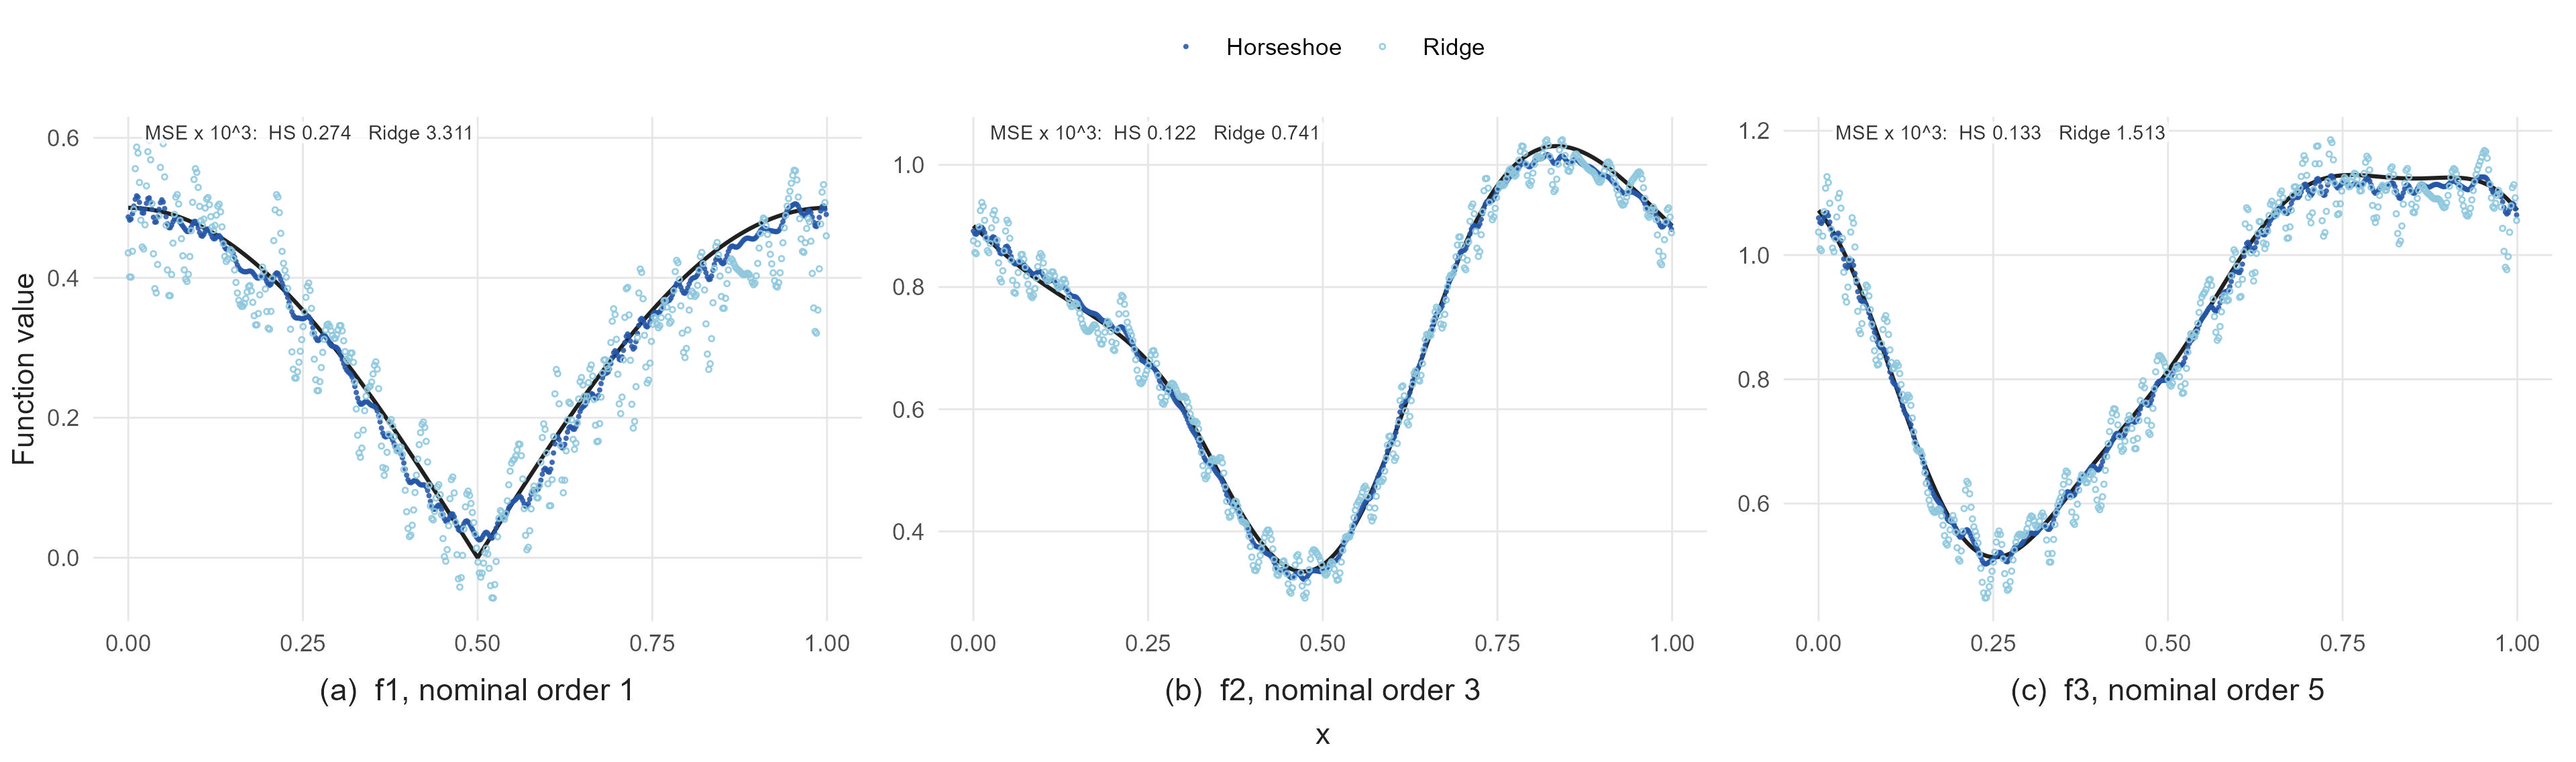
\includegraphics[width=\textwidth]{Ridge_Hs/ridge_hs_trend_comparison.jpg}
\caption{Fourier fits for the three benchmark functions in one simulated data set.  The black curves are the true functions, the dark-blue filled points are the Horseshoe posterior means, and the light-blue open points are the cross-validated ridge estimates.  The in-panel annotations report design-point MSE multiplied by $10^3$.  All panels use $n=1000$ and $J_n=\lfloor n^{0.7}\rfloor=125$.}
\label{fig:fourier-estimates}
\end{figure}

Figure~\ref{fig:fourier-estimates} shows one realization. At $J_n=125$, the Horseshoe and ridge MSE values, multiplied by $10^3$, are $0.274$ and $3.311$ for $f_1$, $0.122$ and $0.741$ for $f_2$, and $0.133$ and $1.513$ for $f_3$, so the Horseshoe error is roughly six to twelve times smaller. The Horseshoe estimates stay closer to the target curves, while the ridge estimates show larger local deviations, especially for $f_1$ and $f_3$.

We next hold $n=1000$ fixed and vary the Fourier dictionary size over
$J_n\in\{140,160,\ldots,300\}$. For a fitted curve $\widehat f$, the design-point error is
\begin{align*}
\operatorname{MSE}(\widehat f)
=\frac1n\sum_{i=1}^n\{\widehat f(x_i)-f_0(x_i)\}^2.
\end{align*}

\begin{table}[ht]
\centering
\small
\setlength{\tabcolsep}{3pt}
\caption{Design-point MSE, multiplied by $10^3$, across Fourier dictionary sizes; one simulated response per target, reused for every $J_n$. Boldface marks the lower value in each pair.}
\label{tab:mse}
\begin{tabular}{llrrrrrrrrr}
\toprule
 & & \multicolumn{9}{c}{Dictionary size $J_n$} \\
\cmidrule(lr){3-11}
$f$ & Method
& 140 & 160 & 180 & 200 & 220 & 240 & 260 & 280 & 300 \\
\midrule
\multirow{2}{*}{$f_1$}
& Horseshoe
& \textbf{0.285} & \textbf{0.315} & \textbf{0.294} & \textbf{0.302} & \textbf{0.294} & \textbf{0.299} & \textbf{0.276} & \textbf{0.271} & \textbf{0.279} \\
& Ridge
& 3.746 & 4.245 & 4.714 & 5.150 & 5.579 & 5.982 & 6.440 & 6.819 & 7.383 \\
\midrule
\multirow{2}{*}{$f_2$}
& Horseshoe
& \textbf{0.126} & \textbf{0.131} & \textbf{0.130} & \textbf{0.133} & \textbf{0.128} & \textbf{0.133} & \textbf{0.130} & \textbf{0.129} & \textbf{0.131} \\
& Ridge
& 0.844 & 0.968 & 1.083 & 1.194 & 1.304 & 1.404 & 1.525 & 1.625 & 1.782 \\
\midrule
\multirow{2}{*}{$f_3$}
& Horseshoe
& \textbf{0.140} & \textbf{0.153} & \textbf{0.145} & \textbf{0.151} & \textbf{0.142} & \textbf{0.146} & \textbf{0.138} & \textbf{0.127} & \textbf{0.136} \\
& Ridge
& 1.723 & 1.983 & 2.209 & 2.443 & 2.659 & 2.871 & 3.115 & 3.320 & 3.640 \\
\bottomrule
\end{tabular}
\end{table}

On the $10^3\times\operatorname{MSE}$ scale of Table~\ref{tab:mse}, the Horseshoe values range from $0.271$ to $0.315$, from $0.126$ to $0.133$, and from $0.127$ to $0.153$ for $f_1,f_2,f_3$, respectively, while the ridge values range from $3.746$ to $7.383$, from $0.844$ to $1.782$, and from $1.723$ to $3.640$. The ridge error grows steadily with $J_n$, roughly doubling between $J_n=140$ and $J_n=300$, whereas the Horseshoe error stays essentially flat: over this range, enlarging the dictionary does not hurt the Horseshoe, which is exactly the behavior the large series prior relies on. The Horseshoe has the lower error in all $27$ comparisons.

\subsection{Empirical scaling of point estimators}\label{sec:convergence}

The scaling experiment uses three periodic targets of nominal regularity $m=1,3,5$, labelled $f_1,f_2,f_3$ in Table~\ref{tab:convergence}, with $J_n=\lfloor n^{0.7}\rfloor$ and the sample sizes $n=1000,1500,\ldots,20000$. Two numerical bases are used: the cosine basis $1,\cos(\pi x),\ldots,\cos(\pi J_nx)$, with $J_n+1$ columns, and a single-resolution cubic B-spline basis with $J_n$ columns and equally spaced knots. Posterior inference uses the Horseshoe with a practical global scale rather than the $\tau_n$ of Section~\ref{sec:contraction} (Remark~\ref{rem:practical}), and treats $\sigma^2$ as known. For each $n$, independent data sets are generated; in each, the coefficientwise posterior mean is reconstructed as a function and its error is measured by
\begin{align*}
\operatorname{RMSE}(\widehat f)=\|\widehat f-f_0\|_{2,n},
\end{align*}
the square root of the design-point MSE of Section~\ref{sec:benchmarks}, so that slopes are on the scale of $\epsilon_n$. At each $n$, the RMSE values are summarized by their median across data sets.

\subsubsection{Rate-scale comparison}

For each function and basis, we regress the logarithm of the median RMSE on $\log n$. Under the hypotheses of Remark~\ref{rem:polynomial}, $\epsilon_n\asymp\sqrt{\log n}\,n^{(\gamma-1)/2}$; we therefore also report the slope for the response $\log(\operatorname{RMSE})-\tfrac12\log\log n$. 

\subsubsection{Thresholded coefficient counts}

For data set $\ell$, define the coefficient count
\begin{align*}
\widehat q_{n,\ell}
=\sum_{j}
\mathbf 1\!\left\{|\widehat\theta^{\,\mathrm{mean}}_{j,n,\ell}|>\frac1{J_n}\right\},
\end{align*}
where the sum runs over all columns of the basis. We take its median across data sets and denote by $\widehat\gamma_q$ the slope from regressing $\log\widehat q_n$ on $\log n$. The count $\widehat q_n$ is our estimate of the sparsity level. In the theory, a coefficient is non-negligible when it exceeds $\delta_n=c_\delta\en/J_n=o(1/J_n)$, a threshold calibrated to the strong shrinkage of the theoretical global scale $\tau_n$. Scales that small make the Gibbs sampler numerically unstable for large $n$; in our runs, instability appears once $\tau$ falls much below $1/J_n^{2}$. The practical scale therefore shrinks less, and we use the correspondingly larger threshold $1/J_n$. For the same reason, $\widehat\gamma_q$ is an empirical proxy for the sparsity exponent $\gamma$ of Remark~\ref{rem:polynomial} rather than an estimate of the $a_n$ of Assumption~\ref{ass:sparse}.

\begin{table}[ht]
\centering
\caption{Empirical log--log slopes for the coefficient-wise posterior mean on the grid $n=1000,1500,\ldots,20000$. Raw: response $\log(\mathrm{RMSE})$. Adjusted: response $\log(\mathrm{RMSE})-\tfrac12\log\log n$. $\widehat\gamma_q$: slope of the $1/J_n$ coefficient count. Implied: the exponent $(\widehat\gamma_q-1)/2$ of Remark~\ref{rem:polynomial} evaluated at $\gamma=\widehat\gamma_q$.}
\label{tab:convergence}
\begin{tabular}{llcccc}
\toprule
$f$ & Basis & Raw & Adjusted & $\widehat\gamma_q$ & Implied \\
\midrule
\multirow{2}{*}{$f_1$ ($m=1$)}
& B-spline & $-0.151$ & $-0.210$ & $0.707$ & $-0.147$ \\
& Cosine   & $-0.332$ & $-0.390$ & $0.241$ & $-0.380$ \\
\midrule
\multirow{2}{*}{$f_2$ ($m=3$)}
& B-spline & $-0.145$ & $-0.203$ & $0.718$ & $-0.141$ \\
& Cosine   & $-0.339$ & $-0.397$ & $0.251$ & $-0.375$ \\
\midrule
\multirow{2}{*}{$f_3$ ($m=5$)}
& B-spline & $-0.124$ & $-0.182$ & $0.747$ & $-0.127$ \\
& Cosine   & $-0.327$ & $-0.385$ & $0.225$ & $-0.388$ \\
\bottomrule
\end{tabular}
\end{table}

The slopes in Table~\ref{tab:convergence} are set by the basis rather than by the smoothness of the target: the three targets give nearly the same slope within each basis, while the two bases differ sharply. The coefficient counts account for the difference. The cosine fits stay sparse, with $\widehat\gamma_q$ between $0.225$ and $0.251$, whereas the B-spline count grows essentially as fast as $J_n=\lfloor n^{0.7}\rfloor$ itself, as expected for a single-resolution basis (Remark~\ref{rem:practical}). The exponent implied by these counts through Remark~\ref{rem:polynomial} lies within about $0.06$ of both observed slopes in every row. These results suggest that the main driver of the convergence rate is the sparsity associated with the basis system, which could also be explained by the nature of their support, global for the cosine basis and local for the B-splines.

The slopes need not match the minimax exponents of Corollary~\ref{cor:anisotropic}, even for the cosine basis. First, the practical global scale shrinks less than $\tau_n$, so the fits are less sparse than Theorem~\ref{thm:main} assumes, and the slopes reflect the sparsity the sampler actually attains rather than the smoothness of $f_0$. Second, $n\leq20{,}000$ is a reasonably large but finite range, so the slopes describe finite-sample behavior rather than the limiting rate.

\subsection{Real-data applications}
\label{sec:applications}

We apply the large series prior to three publicly available series, each visibly noisy, whose mean functions differ markedly in complexity.
\begin{itemize}
\item \emph{Sunspots}: the monthly mean total sunspot number from January 1900 to December 2024 \citep{SILSO,Clette2014}, so $n=1{,}500$. It is used on the square-root scale, which approximately stabilizes the variance of counts.
\item \emph{Bike rentals}: daily rentals, in thousands, in the Capital Bikeshare system of Washington, DC, in 2011--2012 \citep{FanaeeT2014,UCIBike}, so $n=731$.
\item \emph{Wave height}: logarithms of daily mean significant wave heights at NOAA buoy 46001 in the Gulf of Alaska, 2010--2023 \citep{NDBC46001}. One day per week is retained; about $11\%$ of these dates have no valid daily mean and are omitted, so $n=650$. The days are indexed by day of the year.
\end{itemize}

In each case the covariate is rescaled to $[0,1]$ and the frequency cutoff is $F_n=\lfloor n^{0.7}\rfloor$, that is $167$, $101$, and $93$. For the wave heights, day of the year is a periodic covariate, and the dictionary is the real Fourier basis with $F_n$ frequencies, so $J_n=2F_n+1$. The two chronological series begin and end at different levels, which a periodic expansion would force to agree. For them we use the constant and the cosines $\cos(\pi kx)$, $k=1,\ldots,2F_n$. This dictionary has the same size and the same highest frequency, does not force equal endpoint values, and instead has zero slope at both ends. Because $\lfloor n^{0.7}\rfloor$ is here a frequency cutoff rather than a number of columns, $J_n$ is about twice the size used in Section~\ref{sec:benchmarks}.

In all three cases, Horseshoe priors are placed on the $J_n$ coefficients with the global scale fixed at $\tau=F_n^{-2}$, and the noise scale has the Jeffreys prior $\pi(\sigma)\propto\sigma^{-1}$. The same rules for $F_n$ and $\tau$ are used for all three series. Posterior summaries use $20{,}000$ draws after $10{,}000$ burn-in iterations of one chain, and the reported curve is the posterior mean of $f$.

\begin{figure}[!tbp]
\centering
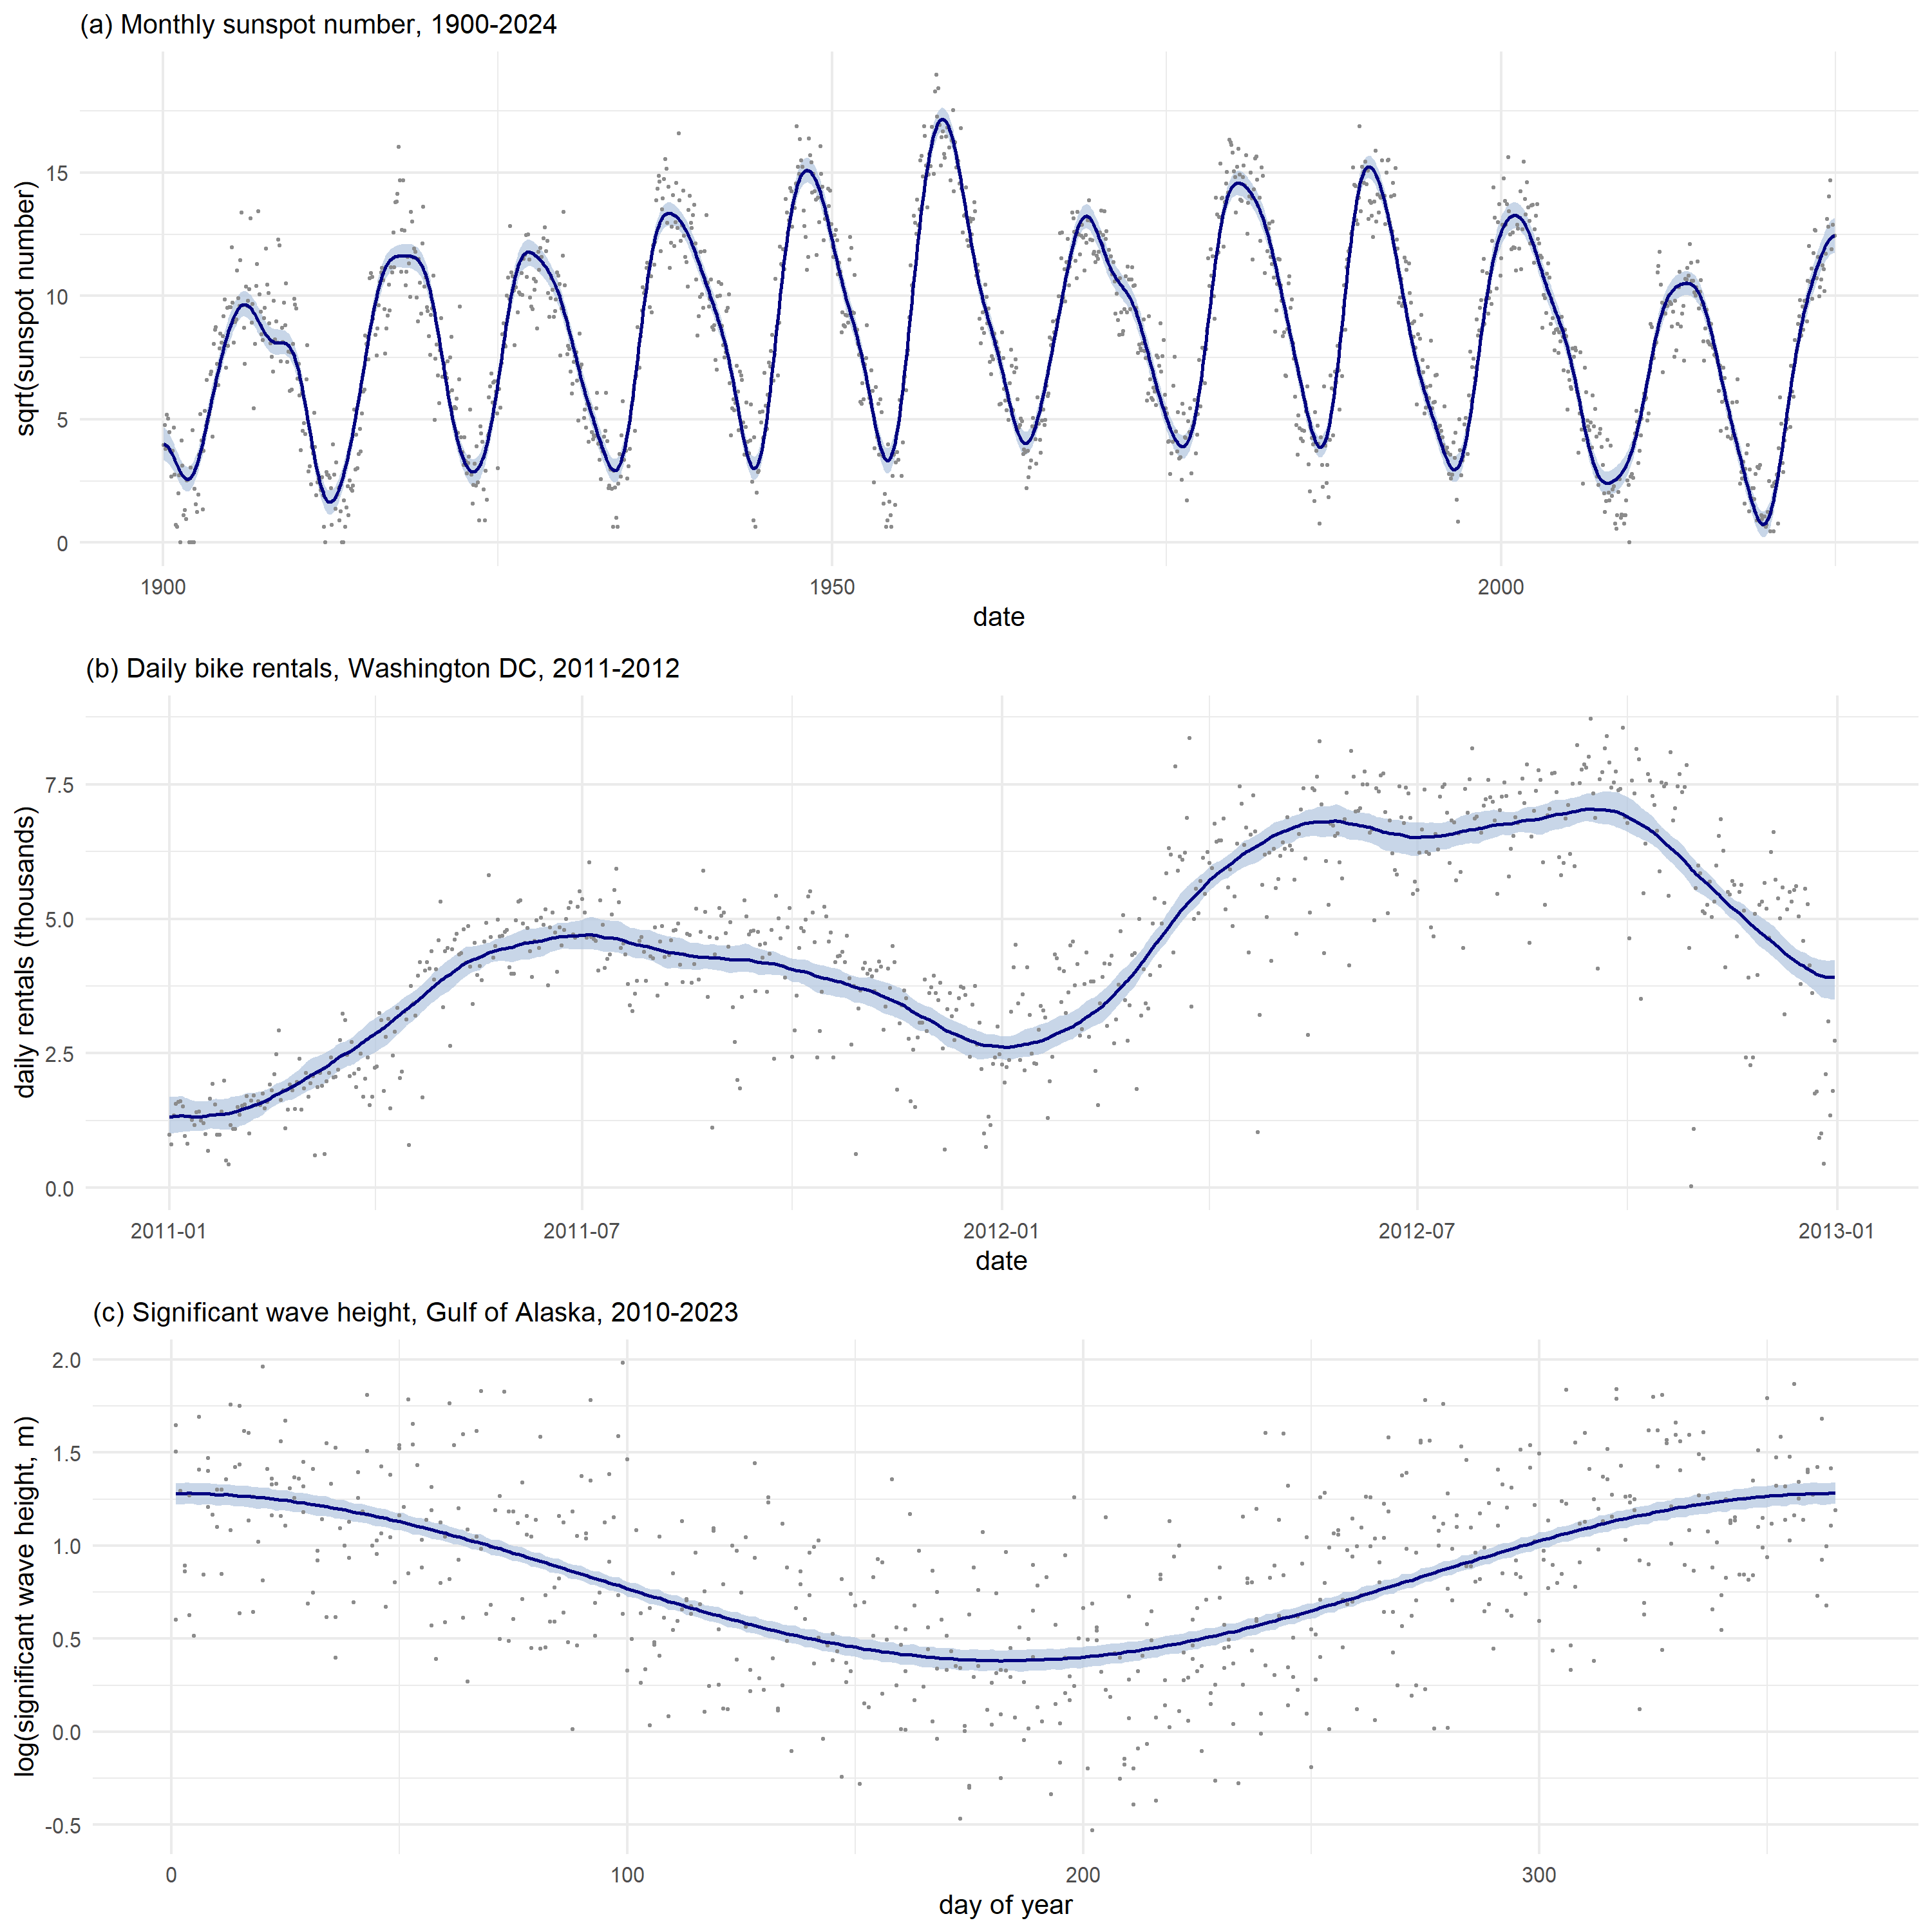
\includegraphics[width=\textwidth]{applications_fig.png}
\caption{Horseshoe fits with the dictionaries described in Section~\ref{sec:applications}, using the frequency cutoff $F_n=\lfloor n^{0.7}\rfloor$ and $\tau=F_n^{-2}$. Gray points are the data, curves are posterior means of the mean function, and shaded bands are pointwise $95\%$ credible bands for it.}
\label{fig:applications}
\end{figure}

Figure~\ref{fig:applications} shows the three fits. In each case the posterior mean is smooth and follows the systematic part of the series rather than its scatter:
\begin{itemize}
\item for the sunspots, the solar cycles with their varying length and amplitude;
\item for the bike rentals, the growth of the system over the two years together with its seasonal pattern;
\item for the wave heights, a single annual cycle, with rough winters and calm summers.
\end{itemize}
No series required its own choice of the number of terms: the dictionary size and the global scale follow the same rule throughout, and the shrinkage prior selects the effective complexity of each fit.



\section{Conclusion}\label{sec-conc}

This paper proposes a large series prior for Bayesian nonparametric regression: a deterministic number of basis functions growing as $n^b$, combined with a shrinkage prior on the coefficients. Theorem~\ref{thm:main} gives posterior contraction rates for product shrinkage priors that satisfy prior-mass conditions adapted from \citet{WeiGhosal2020}, with general dictionaries, and shows that the posterior concentrates on coefficient vectors with at most a multiple of $s_n$ coordinates above the negligibility threshold.

Under the sparse approximation profile and the prior conditions of Corollary~\ref{cor:anisotropic}, the posterior contracts at the rate $(n/\log n)^{-\alpha/(2\alpha+1)}$ for $f_0\in C^\alpha([0,1])$, the minimax rate up to a logarithmic factor, and concentrates on coefficient vectors with at most a fixed multiple of $(n/\log n)^{1/(2\alpha+1)}$ coordinates exceeding $\delta_n$ in absolute value. In $d$ dimensions the rate is $(n/\log n)^{-\alpha/(2\alpha+d)}$ and the support bound is a fixed multiple of $(n/\log n)^{d/(2\alpha+d)}$; under anisotropic smoothness, $\alpha$ is replaced by the harmonic mean $\alpha^*$ of the directional smoothness parameters. These conclusions apply to the classes of Lemmas~\ref{lem:bspline-profile} and~\ref{lem:fourier-profile}: periodic functions for the Fourier dictionary, and smoothness at most the spline order, with integer directional smoothness in the anisotropic case, for the multiresolution B-spline dictionary. The Horseshoe with a deterministic global scale satisfies the prior conditions, and its scale does not depend on the smoothness, so one prior attains these rates pointwise over the admissible range. More broadly, the rate is governed by the sparsity with which the dictionary represents $f_0$ (Remark~\ref{rem:polynomial}), so a basis system matters mainly through the sparsity it induces.

The numerical results support this picture. On a common Fourier dictionary, the Horseshoe has a lower error than cross-validated ridge regression in every comparison, and its error stays essentially flat as the dictionary grows, while the ridge error roughly doubles. In the scaling experiment, the empirical error decay follows the sparsity of the fitted coefficients, and the basis system, rather than the smoothness of the target, separates the rates. In the three real-data applications, one rule for the dictionary size and the global scale yields smooth fits of very different complexity. A natural next step is a sampler that remains stable at the very small global scales the theory calls for, which would bring the simulations closer to the regime of Theorem~\ref{thm:main}.


\bibliography{refs}

\newpage
\section*{Appendix}

The Appendix is organized as follows. The proofs of Theorem~\ref{thm:main} and Corollary~\ref{cor:anisotropic} follow, together with the formal description of the admissible smoothness ranges. Both proofs have the same layout: the supporting lemmas are stated first, the result is proved from them, the lemmas are proved next, and the conditions on $n$ used along the way are collected at the end. The Appendix closes with the statements and proofs of the two sparse approximation lemmas invoked in Section~\ref{sec:adaptive-rates}.

\subsection*{Proof of Theorem~\ref{thm:main}}

The proof follows the testing approach of \citet{Ghosal2000} and \citet{Ghosal2007} and rests on four estimates, stated below as Lemmas~\ref{lem:local-mass}--\ref{lem:tests}: a lower bound on the prior mass of a prediction ball around $f_0$; a lower bound on the evidence $D_n$ holding with high $P_0$-probability; an upper bound on the prior mass of the non-sparse coefficient vectors; and tests separating $f_0$ from the sparse vectors whose prediction lies farther than $M_n\epsilon_n$ from $f_0$. Given the four lemmas, the theorem is proved immediately after them. The lemmas are proved next; the last of them rests on a basic Gaussian test, an elementary packing bound, and a covering of the prediction-distance shells.

\subsubsection*{Preliminaries}

\paragraph*{Likelihood, evidence, and posterior.}
Throughout, a function is identified with its evaluation vector in $\R^n$, and all balls, projections, and coverings take place in $(\R^n,\langle\cdot,\cdot\rangle_n)$. Set
\begin{align*}
L_n(\theta)=\frac{p_\theta}{p_0}(Y^{(n)}),
\qquad
D_n=\int_{\R^{J_n}}L_n(\theta)\,d\Pi_n(\theta).
\end{align*}
For every Borel set $H\subset\R^{J_n}$, Bayes' formula reads
\begin{align}
\Post{H}=\frac{\int_HL_n(\theta)\,d\Pi_n(\theta)}{D_n}.
\label{eq:bayes}
\end{align}
In line with the induced-prior convention of Section~\ref{sec:prior-def}, a prior or posterior probability of a set of functions is the probability of the set of coefficient vectors realizing those functions; in particular $\Post{\emp{f-f_0}>M_n\epsilon_n}$ means $\Post{\{\theta:\emp{f_\theta-f_0}>M_n\epsilon_n\}}$, and no uniqueness of the coefficient representation is ever used. The map $(\theta,y)\mapsto(p_\theta/p_0)(y)$ is continuous and strictly positive, so $D_n$ is a measurable function of the data, $D_n>0$ for every data vector, and, by Tonelli's theorem and $\int p_\theta(y)\,dy=1$, $E_0D_n=\int E_0L_n(\theta)\,d\Pi_n(\theta)=1$; hence $D_n<\infty$ $P_0$-almost surely and~\eqref{eq:bayes} is well defined; on the $P_0$-null set $\{D_n=\infty\}$ the posterior may be defined arbitrarily, and nothing below depends on that choice. For the same reason, the posterior probability of any Borel coefficient set is a measurable function of $Y^{(n)}$.

The proof of our main result relies on the following facts, constants, and lemmas.

\begin{fact}[Rate relations]\label{fact:rates}
Under~\eqref{sparsity} and~\eqref{eq:standing-sequences}, and with $J_n\geq2$ and $J_n\to\infty$ as in Section~\ref{sec:prior-def}, for every $n$,
\begin{align}
0<\en\leq\epsilon_n,
\qquad
n\epsilon_n^2=s_n\log J_n\geq\log2,
\label{eq:rate-relations}
\end{align}
and, as $n\to\infty$,
\begin{align}
n\epsilon_n^2\to\infty,\qquad
\epsilon_n\to0,\qquad
\en\to0 .
\label{eq:rate-limits}
\end{align}
\end{fact}


The rate $\en$ governs the prior mass near $f_0$ and the evidence, whereas $\epsilon_n$ governs the sparse sieve and the tests and is the contraction rate; the inequality $\en\leq\epsilon_n$ is what allows the two groups of estimates to be combined.

\paragraph*{Constants.}
The proof uses the following constants, each depending only on the ones before it:
\begin{gather}
\widetilde L=1+K(1+2\eta),
\qquad
C_0=\frac{\sqrt2\,\widetilde L}{\sigma}+\frac{\widetilde L^2}{2\sigma^2},
\qquad
C_\Pi=c_4+c_5+1,
\label{eq:constants}\\
C_1=C_\Pi+C_0,
\qquad
A=\left\lceil\frac{C_1+1}{\mu}\right\rceil .
\label{eq:constants-A}
\end{gather}
Thus $A$ is a positive integer depending only on $(K,\sigma,\mu,\eta,c_4,c_5)$, as required in Theorem~\ref{thm:main}, and $\mu A\geq C_1+1$.

\begin{fact}[Gaussian tail bound]\label{fact:gauss}
If $X\sim N(0,\tau^2)$ with $\tau>0$, then for every $t\geq0$,
\begin{align}
\Pr\{X\geq t\}\leq e^{-t^2/(2\tau^2)},
\qquad
\Pr\{X\leq-t\}\leq e^{-t^2/(2\tau^2)} .
\label{eq:gausstail}
\end{align}
\end{fact}

\begin{fact}[Change of measure]\label{fact:com}
For every $\theta\in\R^{J_n}$ and every nonnegative measurable function $h$ on $\R^n$,
\begin{align}
E_0\{L_n(\theta)\,h(Y^{(n)})\}=E_{f_\theta}h(Y^{(n)}).
\label{eq:com}
\end{align}
\end{fact}


\paragraph*{Three coefficient sets.}
With $A$ the integer in~\eqref{eq:constants-A}, let
\begin{align}
N(\theta)&=\#\{j:|\theta_j|>\delta_n\},
&\Theta_n&=\{\theta:N(\theta)\leq As_n\},
\label{eq:sieve-def}\\
&&B_n&=\{\theta:\emp{f_\theta-f_0}\leq\widetilde L\en\},
\label{eq:ball-def}\\
&&U_n&=\{\theta:\emp{f_\theta-f_0}>M_n\epsilon_n\}.
\label{eq:far-def}
\end{align}
The \emph{sieve} $\Theta_n$ consists of the \emph{sparse} coefficient vectors, those with at most $As_n$ non-negligible coordinates; its complement is exactly the event in~\eqref{eq:main-support-L1}. The \emph{local ball} $B_n$ is the neighborhood of $f_0$ whose prior mass drives the evidence. The set $U_n$ is the event in~\eqref{eq:main-L1}. All three are Borel sets: $N$ is a finite sum of indicators of open sets, and $\theta\mapsto f_\theta$ is linear. Finally, $W_n=\{f_\theta:\theta\in\Theta_n\}$ denotes the set of functions with at least one sparse representative.

\subsubsection*{The four estimates}

\begin{auxlemma}[Local prior mass]\label{lem:local-mass}
For all sufficiently large $n$,
\begin{align}
\Pi_n(B_n)\geq e^{-C_\Pi n\en^2}.
\label{eq:local-mass}
\end{align}
\end{auxlemma}

\begin{auxlemma}[Evidence lower bound]\label{lem:evidence}
For all sufficiently large $n$,
\begin{align}
P_0\{D_n<e^{-C_1n\en^2}\}\leq e^{-n\en^2}.
\label{eq:evidence}
\end{align}
\end{auxlemma}

\begin{auxlemma}[Prior mass of the sieve complement]\label{lem:sieve}
For every $n$ for which~\eqref{eq:3} holds,
\begin{align}
\Pi_n(\Theta_n^c)=\Pi_n\{N(\theta)>As_n\}
\leq e^{-\mu As_n\log J_n}
=e^{-\mu An\epsilon_n^2}.
\label{eq:sieve-mass}
\end{align}
\end{auxlemma}

\begin{auxlemma}[Tests]\label{lem:tests}
There exist measurable tests $\phi_n=\phi_n(Y^{(n)})\in\{0,1\}$ such that, for all sufficiently large $n$,
\begin{align}
E_0\phi_n&\leq2e^{-n\epsilon_n^2},
\label{eq:type-I}\\
\sup_{\theta\in\Theta_n\cap U_n}E_{f_\theta}(1-\phi_n)
&\leq\exp\Big\{-\frac{M_n^2n\epsilon_n^2}{64\sigma^2}\Big\}.
\label{eq:type-II}
\end{align}
The construction uses the eventual conditions $M_n\geq16K$ and $\log J_n\geq1+\log97$, and the Type~I bound~\eqref{eq:type-I} uses $M_n^2\geq16\sigma^2(2A+1)$.
\end{auxlemma}

The hypotheses enter as follows. Assumption~\ref{ass:sparse} and conditions~\eqref{eq:4}--\eqref{eq:5} are used only in Lemma~\ref{lem:local-mass}; condition~\eqref{eq:3} is used in Lemma~\ref{lem:sieve} and in one case of Lemma~\ref{lem:local-mass}; Assumption~\ref{ass:basis} and the threshold requirement $\delta_n\leq\en/J_n$ are used in Lemmas~\ref{lem:local-mass} and~\ref{lem:tests}; the Gaussian form of the model is used in Lemmas~\ref{lem:evidence} and~\ref{lem:tests}. Lemma~\ref{lem:sieve} holds for every integer $A\geq1$; the specific choice~\eqref{eq:constants-A} is what makes the sieve bound survive division by the evidence bound.

\subsubsection*{Proof of the theorem from the four estimates}

\begin{proof}[Proof of Theorem~\ref{thm:main}]
Let $d_n^*=e^{-C_1n\en^2}$, let $Z_n=\Post{U_n}$ be the posterior probability in~\eqref{eq:main-L1}, and let $\phi_n$ be the tests of Lemma~\ref{lem:tests}. Splitting $1=\phi_n+(1-\phi_n)$, then splitting $1-\phi_n$ according to the event $\{D_n<d_n^*\}$ and its complement, and using $0\leq Z_n\leq1$,
\begin{align}
E_0Z_n
&=E_0(\phi_nZ_n)
 +E_0\{(1-\phi_n)\mathbf1\{D_n<d_n^*\}Z_n\}
 +E_0\{(1-\phi_n)\mathbf1\{D_n\geq d_n^*\}Z_n\}\notag\\
&\leq E_0\phi_n+P_0(D_n<d_n^*)+R_n,
\label{eq:decomposition}
\end{align}
where $R_n$ denotes the last expectation. By~\eqref{eq:type-I} and~\eqref{eq:evidence}, the first two terms are at most $2e^{-n\epsilon_n^2}$ and $e^{-n\en^2}$.

To bound $R_n$, note that $\Theta_n^c$ and $U_n\cap\Theta_n$ are disjoint and their union contains $U_n$. On the event $\{D_n\geq d_n^*\}$, by~\eqref{eq:bayes}, $L_n\geq0$, and $0\leq1-\phi_n\leq1$,
\begin{align*}
(1-\phi_n)Z_n
\leq\frac1{d_n^*}\Big[
 \int_{\Theta_n^c}L_n(\theta)\,d\Pi_n(\theta)
 +\int_{U_n\cap\Theta_n}(1-\phi_n)L_n(\theta)\,d\Pi_n(\theta)
 \Big],
\end{align*}
where $1-\phi_n$, a function of the data alone, was moved inside the second integral and dropped from the first. Take $E_0$, discard the indicator of $\{D_n\geq d_n^*\}$, and apply Tonelli's theorem, legitimate because the integrands are nonnegative and jointly measurable in $(\theta,y)$, together with~\eqref{eq:com} for $h=1$ and $h=1-\phi_n$:
\begin{align}
R_n
\leq e^{C_1n\en^2}\Big[
\Pi_n(\Theta_n^c)
+\int_{U_n\cap\Theta_n}E_{f_\theta}(1-\phi_n)\,d\Pi_n(\theta)
\Big].
\label{eq:remainder}
\end{align}
The two terms in brackets are controlled by Lemmas~\ref{lem:sieve} and~\ref{lem:tests}. By~\eqref{eq:sieve-mass}, $\en\leq\epsilon_n$, and $\mu A\geq C_1+1$,
\begin{align}
e^{C_1n\en^2}\Pi_n(\Theta_n^c)
\leq\exp\{C_1n\epsilon_n^2-\mu An\epsilon_n^2\}
\leq e^{-n\epsilon_n^2}.
\label{eq:sieve-after-evidence}
\end{align}
Offsetting the factor $e^{C_1n\en^2}$ is the purpose of the choice of $A$ in~\eqref{eq:constants-A}. By~\eqref{eq:type-II}, $\Pi_n(U_n\cap\Theta_n)\leq1$, and again $\en\leq\epsilon_n$,
\begin{align*}
e^{C_1n\en^2}\int_{U_n\cap\Theta_n}E_{f_\theta}(1-\phi_n)\,d\Pi_n(\theta)
\leq\exp\Big\{-\Big(\frac{M_n^2}{64\sigma^2}-C_1\Big)n\epsilon_n^2\Big\}
\leq e^{-n\epsilon_n^2},
\end{align*}
once $M_n^2\geq64\sigma^2(C_1+1)$. Collecting the four bounds in~\eqref{eq:decomposition} and using $e^{-n\epsilon_n^2}\leq e^{-n\en^2}$,
\begin{align*}
E_0Z_n
\leq2e^{-n\epsilon_n^2}+e^{-n\en^2}+e^{-n\epsilon_n^2}+e^{-n\epsilon_n^2}
\leq5e^{-n\en^2}
\leq6e^{-n\en^2},
\end{align*}
which is~\eqref{eq:main-L1}.

For the support assertion let $Q_n=\Post{\Theta_n^c}$, the posterior probability in~\eqref{eq:main-support-L1}. No test is needed, because Lemma~\ref{lem:sieve} bounds the prior mass of the whole set $\Theta_n^c$ and the choice of $A$ alone offsets the factor $1/d_n^*$. Splitting according to $\{D_n<d_n^*\}$ as in~\eqref{eq:decomposition} with $\phi_n\equiv0$, and using~\eqref{eq:com} with $h=1$ and then~\eqref{eq:sieve-after-evidence},
\begin{align*}
E_0Q_n
\leq P_0(D_n<d_n^*)+e^{C_1n\en^2}\Pi_n(\Theta_n^c)
\leq e^{-n\en^2}+e^{-n\epsilon_n^2}
\leq2e^{-n\en^2}.
\end{align*}

Finally, for every fixed $\zeta>0$, Markov's inequality gives
\begin{align*}
P_0(Z_n>\zeta)\leq\frac5\zeta e^{-n\en^2}\to0,
\qquad
P_0(Q_n>\zeta)\leq\frac2\zeta e^{-n\en^2}\to0,
\end{align*}
because $n\en^2\to\infty$. The first limit is~\eqref{eq:main-contraction}, posterior contraction at the rate $\epsilon_n$; the second is the corresponding statement for the effective support.
\end{proof}

\subsubsection*{Proof of Lemma~\ref{lem:local-mass}: local prior mass}

\begin{proof}
Let $\theta_0$ and $\xi_n^*$ be the approximant and the set of $a_n$ indices fixed in Assumption~\ref{ass:sparse}, and put
\begin{align*}
h_n=\frac{\eta\en}{a_n}.
\end{align*}
By the triangle inequality, linearity of $\theta\mapsto f_\theta$, Assumption~\ref{ass:basis}, and~\eqref{approx}, an $\ell_1$ coefficient error translates into a prediction error:
\begin{align}
\emp{f_\theta-f_0}
&\leq\emp{f_{\theta_0}-f_0}+\emp{f_\theta-f_{\theta_0}}
\leq\en+\sum_{j=1}^{J_n}|\theta_j-\theta_{0,j}|\emp{\xi_j}\notag\\
&\leq\en+K\|\theta-\theta_0\|_1 .
\label{eq:coefficient-ball}
\end{align}
Since $\en+K(1+2\eta)\en=\widetilde L\en$, it follows that
\begin{align}
\{\theta:\|\theta-\theta_0\|_1\leq(1+2\eta)\en\}\subset B_n,
\label{eq:l1-in-Bn}
\end{align}
and it suffices to bound the prior mass of the left side from below.

We exhibit an event $H_{n,1}\cap H_{n,0}$ inside it, where $H_{n,1}$ constrains the $a_n$ active coordinates $j\in\xi_n^*$ and $H_{n,0}$ constrains the $J_n-a_n$ inactive ones. The two events involve disjoint blocks of coordinates, so they are independent under the product prior and $\Pi_n(H_{n,1}\cap H_{n,0})=\Pi_n(H_{n,1})\Pi_n(H_{n,0})$. For the inactive block take
\begin{align*}
H_{n,0}=\Big\{\sum_{j\notin\xi_n^*}|\theta_j|\leq\eta\en\Big\},
\qquad
\Pi_n(H_{n,0})\geq e^{-c_4n\en^2},
\end{align*}
the bound being condition~\eqref{eq:4} after exponentiation. On $H_{n,0}$, since $|\theta_{0,j}|\leq\delta_n$ for $j\notin\xi_n^*$,
\begin{align}
\sum_{j\notin\xi_n^*}|\theta_j-\theta_{0,j}|
\leq\sum_{j\notin\xi_n^*}|\theta_j|+\sum_{j\notin\xi_n^*}|\theta_{0,j}|
\leq\eta\en+(J_n-a_n)\delta_n .
\label{eq:inactive-block}
\end{align}
The construction of $H_{n,1}$ depends on whether the coefficient bound $E_n$ exceeds the interval length $h_n$. Both cases must be considered because Assumption~\ref{ass:sparse} places no lower bound on $E_n$; if $E_n=E>0$ is fixed, only Case~1 occurs for large $n$, since $a_n\geq1$ gives $h_n\leq\eta\en\to0$. The eventual conditions used below, $\en\leq\eta$, $J_n^\mu\geq2$, and $n\en^2\geq\log2$, are imposed simultaneously, so it is immaterial which case is active for a given $n$.

\smallskip\noindent\emph{Case 1: $E_n\geq h_n$.}
For each $j\in\xi_n^*$ define an inward one-sided interval of length $h_n$,
\begin{align*}
I_j=
\begin{cases}
[\theta_{0,j}-h_n,\theta_{0,j}],&\theta_{0,j}>0,\\
[\theta_{0,j},\theta_{0,j}+h_n],&\theta_{0,j}\leq0,
\end{cases}
\qquad
H_{n,1}=\{\theta_j\in I_j\text{ for every }j\in\xi_n^*\}.
\end{align*}
Each $I_j$ is contained in $[-E_n,E_n]$. When $\theta_{0,j}>0$, the upper endpoint is $\theta_{0,j}\leq E_n$ and the lower endpoint exceeds $-h_n\geq-E_n$. When $\theta_{0,j}\leq0$, the lower endpoint is $\theta_{0,j}\geq-E_n$ and the upper endpoint is at most $h_n\leq E_n$. On $H_{n,1}\cap H_{n,0}$, each active coordinate satisfies $|\theta_j-\theta_{0,j}|\leq h_n$, so the active block contributes at most $a_nh_n=\eta\en$.

Together with~\eqref{eq:inactive-block} and $J_n\delta_n\leq\en$, this gives
\begin{align*}
\|\theta-\theta_0\|_1
\leq\eta\en+\eta\en+(J_n-a_n)\delta_n
\leq(1+2\eta)\en .
\end{align*}
Hence $H_{n,1}\cap H_{n,0}\subset B_n$ by~\eqref{eq:l1-in-Bn}. For the probability of $H_{n,1}$, since $I_j\subset[-E_n,E_n]$ has length $h_n$ and $\pi_n\geq\pinf$ on $[-E_n,E_n]$,
\begin{align*}
\Pi_{n,j}(I_j)=\int_{I_j}\pi_n(t)\,dt\geq h_n\pinf=:b_n>0 .
\end{align*}
By independence of the $a_n$ active coordinates, $\Pi_n(H_{n,1})=\prod_{j\in\xi_n^*}\Pi_{n,j}(I_j)\geq b_n^{a_n}$, so
\begin{align*}
-\log\Pi_n(H_{n,1})
&\leq a_n\log\frac1{b_n}
=a_n\Big[\log a_n+\log\frac1{\eta\en}-\log\pinf\Big]\\
&\leq a_n\Big[\log a_n+2\log\Big(\frac1\en\Big)-\log\pinf\Big]_+
\leq c_5n\en^2 .
\end{align*}
The second inequality uses $\en\leq\eta$, so that $1/(\eta\en)\leq1/\en^2$, together with $x\leq[x]_+$; the last is condition~\eqref{eq:5}. Therefore
\begin{align*}
\Pi_n(B_n)\geq\Pi_n(H_{n,1})\Pi_n(H_{n,0})\geq e^{-(c_4+c_5)n\en^2}.
\end{align*}

\smallskip\noindent\emph{Case 2: $E_n<h_n$.}
Now the active coefficients of the approximant are themselves small, $\sum_{j\in\xi_n^*}|\theta_{0,j}|\leq a_nE_n<a_nh_n=\eta\en$, and it suffices to ask the active coordinates to be negligible:
\begin{align*}
H_{n,1}=\{|\theta_j|\leq\delta_n\text{ for every }j\in\xi_n^*\}.
\end{align*}
On $H_{n,1}\cap H_{n,0}$, by~\eqref{eq:inactive-block} and $J_n\delta_n\leq\en$,
\begin{align*}
\|\theta-\theta_0\|_1
&\leq\sum_{j\in\xi_n^*}|\theta_j|+\sum_{j\in\xi_n^*}|\theta_{0,j}|
  +\eta\en+(J_n-a_n)\delta_n\\
&\leq a_n\delta_n+\eta\en+\eta\en+(J_n-a_n)\delta_n
\leq(1+2\eta)\en,
\end{align*}
so again $H_{n,1}\cap H_{n,0}\subset B_n$. For the probability of $H_{n,1}$, note that $\Pi_{n,j}(|\theta_j|>\delta_n)=\int_{|t|>\delta_n}\pi_n(t)\,dt\leq J_n^{-(1+\mu)}$ by~\eqref{eq:3}; a union bound over the $a_n$ active coordinates, together with $a_n\leq J_n$, gives
\begin{align*}
\Pi_n(H_{n,1})
\geq1-\sum_{j\in\xi_n^*}\Pi_{n,j}(|\theta_j|>\delta_n)
\geq1-a_nJ_n^{-(1+\mu)}
\geq1-J_n^{-\mu}
\geq\frac12,
\end{align*}
the last step once $J_n^\mu\geq2$. Hence
\begin{align*}
\Pi_n(B_n)\geq\frac12e^{-c_4n\en^2}\geq e^{-(c_4+1)n\en^2},
\end{align*}
the last step once $n\en^2\geq\log2$.

In both cases $\Pi_n(B_n)\geq e^{-(c_4+c_5+1)n\en^2}=e^{-C_\Pi n\en^2}$, because $c_5\geq0$ and $1\geq0$. This is~\eqref{eq:local-mass}. The bound requires neither monotonicity nor a positive lower bound for $E_n$.
\end{proof}

\subsubsection*{Proof of Lemma~\ref{lem:evidence}: evidence lower bound}

\begin{proof}
Under $P_0$, write $y_i=f_0(x_i)+\sigma \omega_i$, where $\omega_i=(y_i-f_0(x_i))/\sigma$ are independent standard normal variables, and put $g_\theta=f_\theta-f_0\in\R^n$. The normalizing constants of the Gaussian densities cancel in the ratio, and $(y_i-f_\theta(x_i))^2-(y_i-f_0(x_i))^2=(\sigma \omega_i-g_\theta(x_i))^2-(\sigma \omega_i)^2=-2\sigma \omega_ig_\theta(x_i)+g_\theta(x_i)^2$, so
\begin{align}
\log L_n(\theta)
&=-\frac1{2\sigma^2}\sum_{i=1}^n
\left[(y_i-f_\theta(x_i))^2-(y_i-f_0(x_i))^2\right]\notag\\
&=\frac1\sigma\sum_{i=1}^n\omega_ig_\theta(x_i)-\frac{n}{2\sigma^2}\emp{g_\theta}^2 .
\label{eq:gaussian-lr}
\end{align}
In particular $E_0\log(p_0/p_\theta)=\{n/(2\sigma^2)\}\emp{g_\theta}^2$ and $\operatorname{Var}_0\log(p_0/p_\theta)=(n/\sigma^2)\emp{g_\theta}^2$, so on $B_n$ the Kullback--Leibler divergence and the variance of the log-likelihood ratio are at most $\{\widetilde L^2/(2\sigma^2)\}n\en^2$ and $(\widetilde L^2/\sigma^2)n\en^2$: $B_n$ is a Kullback--Leibler neighborhood of $p_0$ in the sense of \citet{Ghosal2000}. Rather than invoking a generic Kullback--Leibler argument, we use the exact expression~\eqref{eq:gaussian-lr}.

By Lemma~\ref{lem:local-mass}, $\Pi_n(B_n)>0$ for all large $n$, so the prior renormalized to $B_n$, $\Pi_{n,B_n}(H)=\Pi_n(H\cap B_n)/\Pi_n(B_n)$, is a probability measure. On $B_n$ each evaluation satisfies $|g_\theta(x_i)|\leq\{\sum_kg_\theta(x_k)^2\}^{1/2}=\sqrt n\emp{g_\theta}\leq\sqrt n\,\widetilde L\en$, so for each fixed data vector
\begin{align*}
|\log L_n(\theta)|
\leq\frac{\sqrt n\,\widetilde L\en}{\sigma}\sum_{i=1}^n|\omega_i|+\frac{n\widetilde L^2\en^2}{2\sigma^2}
\qquad\text{for all }\theta\in B_n.
\end{align*}
$\log L_n$ is bounded on $B_n$, hence $L_n$ and $\log L_n$ are $\Pi_{n,B_n}$-integrable, and Jensen's inequality for the concave logarithm applies. Restricting the integral defining $D_n$ to $B_n$ (the integrand is positive),
\begin{align*}
\log D_n
\geq\log\Pi_n(B_n)+\log\int L_n(\theta)\,d\Pi_{n,B_n}(\theta)
\geq\log\Pi_n(B_n)+\int\log L_n(\theta)\,d\Pi_{n,B_n}(\theta).
\end{align*}
Inserting~\eqref{eq:gaussian-lr} and exchanging the finite sum over $i$ with the integral,
\begin{align*}
\int\log L_n(\theta)\,d\Pi_{n,B_n}(\theta)
=\frac1\sigma\sum_{i=1}^n\omega_i\bar g(x_i)
 -\frac{n}{2\sigma^2}\int\emp{g_\theta}^2\,d\Pi_{n,B_n}(\theta),
\end{align*}
where $\bar g=\int g_\theta\,d\Pi_{n,B_n}(\theta)\in\R^n$ is the coordinatewise average of the bounded evaluation vectors $g_\theta$, $\theta\in B_n$. The definition of $B_n$ gives the first bound below, and Jensen's inequality for the convex function $\emp\cdot$ (equivalently, $\emp{\int h\,d\nu}\leq\int\emp h\,d\nu$ for a probability measure $\nu$ and an integrable $\R^n$-valued $h$) gives the second:
\begin{align*}
\int\emp{g_\theta}^2\,d\Pi_{n,B_n}(\theta)\leq\widetilde L^2\en^2,
\qquad
\emp{\bar g}\leq\int\emp{g_\theta}\,d\Pi_{n,B_n}(\theta)\leq\widetilde L\en .
\end{align*}

The vector $\bar g$ is determined by $\Pi_n$, $B_n$, $f_0$, and the design, none of which involves the noise, so it is deterministic. Hence $G_n=\sigma^{-1}\sum_i\omega_i\bar g(x_i)$ is, under $P_0$, a centered Gaussian variable with variance
\begin{align*}
v_n=\frac1{\sigma^2}\sum_{i=1}^n\bar g(x_i)^2=\frac{n\emp{\bar g}^2}{\sigma^2}\leq\frac{n\widetilde L^2\en^2}{\sigma^2}.
\end{align*}
Put $t_n^*=\sqrt2\,\widetilde L n\en^2/\sigma>0$. If $v_n=0$ then $G_n=0$ almost surely and $P_0\{G_n<-t_n^*\}=0$. Otherwise, by~\eqref{eq:gausstail} and the bound on $v_n$,
\begin{align*}
P_0\{G_n<-t_n^*\}
\leq\exp\Big\{-\frac{(t_n^*)^2}{2v_n}\Big\}
=\exp\Big\{-\frac{\widetilde L^2n^2\en^4/\sigma^2}{v_n}\Big\}
\leq\exp\Big\{-\frac{\widetilde L^2n^2\en^4/\sigma^2}{n\widetilde L^2\en^2/\sigma^2}\Big\}
=e^{-n\en^2}.
\end{align*}
On the complementary event $\{G_n\geq-t_n^*\}$, combining the three displays above with~\eqref{eq:local-mass},
\begin{align*}
\log D_n
\geq\log\Pi_n(B_n)-\frac{\sqrt2\,\widetilde L}{\sigma}n\en^2-\frac{\widetilde L^2}{2\sigma^2}n\en^2
\geq-C_\Pi n\en^2-C_0n\en^2
=-C_1n\en^2 .
\end{align*}
Thus $\{D_n<e^{-C_1n\en^2}\}\subset\{G_n<-t_n^*\}$, and~\eqref{eq:evidence} follows.
\end{proof}

\subsubsection*{Proof of Lemma~\ref{lem:sieve}: prior mass of the sieve complement}

\begin{proof}
Let $\nu_n=\Pi_{n,j}(|\theta_j|>\delta_n)=\int_{|t|>\delta_n}\pi_n(t)\,dt$ be the common exceedance probability of a coordinate; condition~\eqref{eq:3} gives $\nu_n\leq J_n^{-(1+\mu)}$. If $As_n\geq J_n$, then $N(\theta)\leq J_n\leq As_n$ for every $\theta$, so $\Theta_n^c$ is empty and there is nothing to prove. Otherwise $k=As_n$ is an integer with $1\leq k<J_n$, because $A\geq1$ and $s_n\geq a_n\geq1$ are integers. We claim
\begin{align*}
\{N(\theta)\geq k\}
=\bigcup_{S\subset\{1,\ldots,J_n\}:\,|S|=k}\ \bigcap_{j\in S}\{|\theta_j|>\delta_n\}.
\end{align*}
If $N(\theta)\geq k$, the set of exceeding indices $\{j:|\theta_j|>\delta_n\}$ has at least $k$ elements and therefore contains a subset $S$ of cardinality exactly $k$, and $\theta$ belongs to the intersection indexed by that $S$. Conversely, if $\theta$ belongs to the intersection indexed by some $S$ with $|S|=k$, then $S$ is contained in the set of exceeding indices, so $N(\theta)\geq k$.

For fixed $S$ the events $\{|\theta_j|>\delta_n\}$, $j\in S$, concern distinct coordinates, hence are independent under the product prior, and each has probability $\nu_n$; their intersection has probability $\nu_n^k$. A union bound over the $\binom{J_n}{k}\leq J_n^k$ subsets gives
\begin{align*}
\Pi_n\{N(\theta)\geq k\}
\leq\binom{J_n}{k}\nu_n^k
\leq J_n^kJ_n^{-(1+\mu)k}
=J_n^{-\mu k}.
\end{align*}
With $k=As_n$ and $n\epsilon_n^2=s_n\log J_n$,
\begin{align*}
\Pi_n\{N(\theta)>As_n\}
\leq\Pi_n\{N(\theta)\geq As_n\}
\leq J_n^{-\mu As_n}
=e^{-\mu As_n\log J_n}
=e^{-\mu An\epsilon_n^2}.
\end{align*}
This is~\eqref{eq:sieve-mass}.
\end{proof}

\paragraph*{Prediction-distance shells.}
For each integer $\ell\geq1$, define the $\ell$th shell inside the sieve, with $W_n=\{f_\theta:\theta\in\Theta_n\}$ as in the Preliminaries, as the set of functions
\begin{align}
\mathcal S_\ell=\{f\in W_n:\ell M_n\epsilon_n<\emp{f-f_0}\leq(\ell+1)M_n\epsilon_n\}.
\label{eq:shell}
\end{align}
The shells are pairwise disjoint and their union is $W_n\cap\{f:\emp{f-f_0}>M_n\epsilon_n\}$, because the intervals $(\ell M_n\epsilon_n,(\ell+1)M_n\epsilon_n]$, $\ell\geq1$, partition $(M_n\epsilon_n,\infty)$. Consequently, if $\theta\in\Theta_n\cap U_n$, then $f_\theta\in\mathcal S_\ell$ for exactly one $\ell\geq1$, namely $\ell=\lceil\emp{f_\theta-f_0}/(M_n\epsilon_n)\rceil-1$. Every $f\in\mathcal S_\ell$ has at least one representative $\theta\in\Theta_n\cap U_n$ because $\mathcal S_\ell\subset W_n$, but it may also have non-sparse representatives when the dictionary is redundant; only the forward implication is used.

The covering radius for a shell will be proportional to its distance from $f_0$; this is what permits the neighborhood bound of Lemma~\ref{lem:test} to apply to every point of the shell. The non-negligible coefficients of a sparse vector are not bounded in magnitude, but within a shell their combined prediction is bounded, and once a support is fixed that prediction lies in a subspace of dimension at most the size of the support. We cover this bounded set inside its subspace, using Lemma~\ref{lem:packing}.

\subsubsection*{Proof of Lemma~\ref{lem:tests}: tests}

Lemma~\ref{lem:tests} rests on three ingredients: a test of $f_0$ against a neighborhood of one fixed alternative (Lemma~\ref{lem:test}); an elementary packing bound in a finite-dimensional subspace (Lemma~\ref{lem:packing}); and a covering of the sparse alternatives at prediction distance beyond $M_n\epsilon_n$ by finitely many such neighborhoods, with a controlled number of centers (Lemma~\ref{lem:covering}). The test of Lemma~\ref{lem:tests} rejects if any local test rejects.

\begin{proof}[Proof]
Assume $M_n\geq16K$, $\log J_n\geq1+\log97$, and $M_n^2\geq16\sigma^2(2A+1)$, all of which hold for all sufficiently large $n$ because $M_n\to\infty$ and $J_n\to\infty$. Let the centers $g_{\ell,k}$ be as in Lemma~\ref{lem:covering}, let $\psi_g$ be the test of Lemma~\ref{lem:test}, and define
\begin{align*}
\phi_n=\sup_{\ell\geq1}\ \sup_{1\leq k\leq N_\ell}\psi_{g_{\ell,k}},
\qquad\sup\varnothing:=0,
\end{align*}
which rejects if any local test rejects. Each $\psi_g$ is the indicator of a closed half-space of $\R^n$, so $\phi_n$, the indicator of a countable union of such sets, is measurable. The centers and the tests depend on the fixed truth $f_0$; as is standard in posterior-contraction arguments, $\phi_n$ is an analytic device, not an implementable procedure. By~\eqref{eq:center-away} every center satisfies $d_{\ell,k}:=\emp{g_{\ell,k}-f_0}\geq\frac{15}{16}\ell M_n\epsilon_n>0$, so Lemma~\ref{lem:test} applies to each.

\emph{Type I error.} Since $(15/16)^2=225/256\geq1/2$, Lemma~\ref{lem:test} gives, with $t_n=M_n^2n\epsilon_n^2/(16\sigma^2)$,
\begin{align*}
E_0\psi_{g_{\ell,k}}
\leq\exp\Big\{-\frac{nd_{\ell,k}^2}{8\sigma^2}\Big\}
\leq\exp\Big\{-\frac{(15/16)^2\ell^2M_n^2n\epsilon_n^2}{8\sigma^2}\Big\}
\leq\exp\Big\{-\frac{\ell^2M_n^2n\epsilon_n^2}{16\sigma^2}\Big\}
=e^{-\ell^2t_n}.
\end{align*}
The hypothesis $M_n^2\geq16\sigma^2(2A+1)$ and~\eqref{eq:rate-relations} give $t_n\geq(2A+1)n\epsilon_n^2\geq3\log2>\log2$, hence $(1-e^{-t_n})^{-1}\leq2$. A union bound over the centers, the count~\eqref{eq:center-count}, $\ell^2\geq\ell$, and the geometric series give
\begin{align*}
E_0\phi_n
&\leq\sum_{\ell\geq1}N_\ell e^{-\ell^2t_n}
\leq e^{2An\epsilon_n^2}\sum_{\ell\geq1}e^{-\ell t_n}
=e^{2An\epsilon_n^2}\frac{e^{-t_n}}{1-e^{-t_n}}\\
&\leq2\exp\Big\{-\Big(\frac{M_n^2}{16\sigma^2}-2A\Big)n\epsilon_n^2\Big\}
\leq2e^{-n\epsilon_n^2},
\end{align*}
the last step because $M_n^2/(16\sigma^2)-2A\geq1$. This is~\eqref{eq:type-I}.

\emph{Type II error.} Fix $\theta\in\Theta_n\cap U_n$. Then $f_\theta\in\mathcal S_\ell$ for some $\ell\geq1$, and Lemma~\ref{lem:covering} assigns a center $g_{\ell,k}$ with $\emp{f_\theta-g_{\ell,k}}\leq d_{\ell,k}/4$. Since $\phi_n\geq\psi_{g_{\ell,k}}$ pointwise, Lemma~\ref{lem:test} applied at $v=f_\theta$, followed by $(15/16)^2\geq1/2$ and $\ell\geq1$, gives
\begin{align*}
E_{f_\theta}(1-\phi_n)
\leq E_{f_\theta}(1-\psi_{g_{\ell,k}})
\leq\exp\Big\{-\frac{nd_{\ell,k}^2}{32\sigma^2}\Big\}
\leq\exp\Big\{-\frac{\ell^2M_n^2n\epsilon_n^2}{64\sigma^2}\Big\}
\leq\exp\Big\{-\frac{M_n^2n\epsilon_n^2}{64\sigma^2}\Big\}.
\end{align*}
The bound does not depend on $\theta$, which proves~\eqref{eq:type-II}. Unlike the Type~I calculation, no count of centers is needed: each alternative uses only its one assigned local test.
\end{proof}


\begin{auxlemma}[Basic Gaussian test]\label{lem:test}
Let $g\in\R^n$ with $\varrho:=\emp{g-f_0}>0$, and define
\begin{align*}
T_g=\sum_{i=1}^n(y_i-f_0(x_i))(g_i-f_0(x_i)),
\qquad
\psi_g=\mathbf1\{T_g\geq n\varrho^2/2\}.
\end{align*}
Then
\begin{align*}
E_0\psi_g\leq e^{-n\varrho^2/(8\sigma^2)},
\qquad
\sup_{v\in\R^n:\,\emp{v-g}\leq \varrho/4}E_v(1-\psi_g)\leq e^{-n\varrho^2/(32\sigma^2)} .
\end{align*}
\end{auxlemma}

\begin{proof}
The statistic $T_g$ measures the alignment of the residuals $y_i-f_0(x_i)$ with the fixed direction $g-f_0$. Abbreviate $w_i=g_i-f_0(x_i)$, so that $\sum_{i=1}^nw_i^2=n\emp{g-f_0}^2=n\varrho^2$. Under $P_v$ the observations are $y_i=v_i+\varepsilon_i$, so $y_i-f_0(x_i)=\{v_i-f_0(x_i)\}+\varepsilon_i$ and $T_g$ splits into a deterministic mean and a Gaussian noise term,
\begin{align*}
T_g=m_v+W,
\qquad
m_v=\sum_{i=1}^n\{v_i-f_0(x_i)\}w_i,
\qquad
W=\sum_{i=1}^n\varepsilon_iw_i\sim N(0,\sigma^2n\varrho^2),
\end{align*}
the law of $W$ being that of a linear combination of independent $N(0,\sigma^2)$ variables with fixed coefficients; its variance is positive since $\varrho>0$.

\emph{Type I error.} Under $P_0$ we have $v=f_0$, hence $m_v=0$ and $T_g=W$. By~\eqref{eq:gausstail} with $t=n\varrho^2/2$ and $\tau^2=\sigma^2n\varrho^2$,
\begin{align*}
E_0\psi_g
=\Pr\Big(W\geq\frac{n\varrho^2}{2}\Big)
\leq\exp\Big\{-\frac{(n\varrho^2/2)^2}{2\sigma^2n\varrho^2}\Big\}
=e^{-n\varrho^2/(8\sigma^2)}.
\end{align*}

\emph{Type II error.} Fix $v$ with $\emp{v-g}\leq \varrho/4$. Writing $v_i-f_0(x_i)=(v_i-g_i)+w_i$,
\begin{align*}
m_v&=n\varrho^2+S,
\qquad
S=\sum_{i=1}^n(v_i-g_i)w_i,
\\
|S|&\leq\Big\{\sum_{i=1}^n(v_i-g_i)^2\Big\}^{1/2}\Big\{\sum_{i=1}^nw_i^2\Big\}^{1/2}
=n\emp{v-g}\,\varrho\leq\frac{n\varrho^2}{4},
\end{align*}
by the Cauchy--Schwarz inequality. Hence $m_v\geq3n\varrho^2/4$: the mean of $T_g$ exceeds the rejection threshold $n\varrho^2/2$ by at least $n\varrho^2/4$. The test fails to reject only if the noise $W$ is more negative than this margin, so by~\eqref{eq:gausstail} with $t=n\varrho^2/4$,
\begin{align*}
E_v(1-\psi_g)
&=\Pr\Big(W<\frac{n\varrho^2}{2}-m_v\Big)
\leq\Pr\Big(W\leq-\frac{n\varrho^2}{4}\Big)\\
&\leq\exp\Big\{-\frac{(n\varrho^2/4)^2}{2\sigma^2n\varrho^2}\Big\}
=e^{-n\varrho^2/(32\sigma^2)}.
\end{align*}
The bound depends on $v$ only through the constraint $\emp{v-g}\leq \varrho/4$, so it is uniform over the stated neighborhood.
\end{proof}

\begin{auxlemma}[Packing bound]\label{lem:packing}
Let $V\subset\R^n$ be a linear subspace of dimension $k\geq1$, equipped with $\langle\cdot,\cdot\rangle_n$; let $x\in V$, $R>0$, $r>0$, and let $G\subset V$ be a set of points, each within distance $R$ of $x$, with pairwise distances exceeding $r$. Then $G$ is finite and
\begin{align*}
|G|\leq\Big(1+\frac{2R}{r}\Big)^k .
\end{align*}
Consequently, every nonempty set $F\subset V$ contained in the ball of radius $R$ around $x$ has a finite subset $G\subset F$ with pairwise distances exceeding $r$, of cardinality at most $(1+2R/r)^k$, such that every point of $F$ lies within distance $r$ of some point of $G$.
\end{auxlemma}

\begin{proof}
Choose an orthonormal basis of $V$ for $\langle\cdot,\cdot\rangle_n$; the coordinate map is a linear isometry between $(V,\emp\cdot)$ and Euclidean $\R^k$, under which balls of radius $\rho$ in $V$ correspond to Euclidean balls of radius $\rho$, of Lebesgue volume $c_k\rho^k$ for a constant $c_k>0$. The open balls of radius $r/2$ around the points of $G$ are pairwise disjoint: a point lying in two of them would put two points of $G$ at distance less than $r$. By the triangle inequality each of them lies inside the ball of radius $R+r/2$ around $x$. Comparing volumes of any finite subfamily of $m$ of these balls, $mc_k(r/2)^k\leq c_k(R+r/2)^k$, so $m\leq(1+2R/r)^k$; hence $G$ is finite with the same bound.

For the consequence, the cardinalities of subsets of $F$ with pairwise distances exceeding $r$ are bounded by $(1+2R/r)^k$, and the family of such subsets is nonempty (singletons), so it has a member $G$ of maximal cardinality. If some point $y\in F$ were at distance exceeding $r$ from every point of $G$, then $G\cup\{y\}$ would be a larger such subset; hence every point of $F$ is within $r$ of $G$.
\end{proof}

\begin{auxlemma}[Covering of the shells]\label{lem:covering}
Suppose $M_n\geq16K$ and $\log J_n\geq1+\log97$. Then for every $\ell\geq1$ there are $N_\ell$ centers $g_{\ell,1},\ldots,g_{\ell,N_\ell}\in\R^n$ such that
\begin{align}
\emp{g_{\ell,k}-f_0}\geq\frac{15}{16}\ell M_n\epsilon_n
\qquad(1\leq k\leq N_\ell),
\label{eq:center-away}
\end{align}
every $f\in\mathcal S_\ell$ satisfies, for some $k$,
\begin{align}
\emp{f-g_{\ell,k}}\leq\frac{\ell M_n\epsilon_n}{8}\leq\frac14\emp{g_{\ell,k}-f_0},
\label{eq:center-close}
\end{align}
and, uniformly over $\ell\geq1$,
\begin{align}
N_\ell\leq e^{2As_n\log J_n}=e^{2An\epsilon_n^2}.
\label{eq:center-count}
\end{align}
\end{auxlemma}

\begin{proof}
Fix $\ell\geq1$. The construction proceeds in four steps: remove the negligible coordinates, cover the remaining predictions for each support, combine the supports, and add the negligible coordinates back. The two hypotheses on $M_n$ and $J_n$ do not involve $\ell$, and every inequality in $\ell$ below holds for all $\ell\geq1$; this is the uniformity claimed in~\eqref{eq:center-count}.

\smallskip\noindent\emph{Step 1: remove the negligible coordinates.}
Let $\theta\in\Theta_n$ with $f_\theta\in\mathcal S_\ell$, and put $S(\theta)=\{j:|\theta_j|>\delta_n\}$, a set of size $N(\theta)\leq As_n$. Write $\theta=\theta^{(1)}+\theta^{(2)}$, where $\theta^{(1)}$ agrees with $\theta$ on $S(\theta)$ and vanishes elsewhere, so that $f_\theta=f_{\theta^{(1)}}+f_{\theta^{(2)}}$ and every entry of $\theta^{(2)}$ has magnitude at most $\delta_n$. By the triangle inequality, Assumption~\ref{ass:basis}, the threshold requirement $\delta_n\leq\en/J_n$, and $\en\leq\epsilon_n$,
\begin{align}
\emp{f_{\theta^{(2)}}}
\leq\sum_{j\notin S(\theta)}|\theta_j|\emp{\xi_j}
\leq KJ_n\delta_n
\leq K\en\leq K\epsilon_n
\leq\frac{M_n\epsilon_n}{16},
\label{eq:negligible-part}
\end{align}
the last step by $M_n\geq16K$. Removing the negligible part therefore changes the distance from $f_0$ by at most $M_n\epsilon_n/16$. The two shell bounds and the triangle inequality give
\begin{align}
\frac{15}{16}\ell M_n\epsilon_n
\leq\Big(\ell-\frac1{16}\Big)M_n\epsilon_n
<\emp{f_{\theta^{(1)}}-f_0}
\leq\Big(\ell+1+\frac1{16}\Big)M_n\epsilon_n
\leq(\ell+2)M_n\epsilon_n,
\label{eq:sparse-part-bounds}
\end{align}
where the outer comparisons use $\ell\geq1$. Thus every sparse part arising from the $\ell$th shell lies in a bounded region but remains separated from $f_0$.

\smallskip\noindent\emph{Step 2: cover the sparse parts for one fixed support.}
Fix a support $S\subset\{1,\ldots,J_n\}$ of size $s\leq As_n$, let $V_S$ be the span of the evaluation vectors $\{\xi_j:j\in S\}$, and let $s'=\dim V_S\leq s$, with strict inequality if the vectors are linearly dependent. Consider
\begin{align*}
\mathcal F_{\ell,S}
=\{f_{\theta^{(1)}}:\theta\in\Theta_n,\ f_\theta\in\mathcal S_\ell,\ S(\theta)=S\}
\subset V_S,
\qquad
R_\ell=(\ell+2)M_n\epsilon_n,
\qquad
r_\ell=\frac{\ell M_n\epsilon_n}{16}.
\end{align*}
By~\eqref{eq:sparse-part-bounds}, $\mathcal F_{\ell,S}$ lies in the ball of radius $R_\ell$ around $f_0$. The point $f_0$ need not lie in $V_S$, but if $P_S$ denotes the orthogonal projection onto $V_S$ for $\langle\cdot,\cdot\rangle_n$, then for $v\in V_S$ we have $v-P_Sf_0=P_S(v-f_0)$ and hence $\emp{v-P_Sf_0}\leq\emp{v-f_0}$, since an orthogonal projection does not increase the norm. So $\mathcal F_{\ell,S}$ also lies in the ball of radius $R_\ell$ around the point $P_Sf_0$ of $V_S$.

If $\mathcal F_{\ell,S}$ is empty, use no centers. If $\mathcal F_{\ell,S}$ is nonempty and $s'=0$, then $V_S=\{0\}$, hence $\mathcal F_{\ell,S}=\{0\}$, and we use the single center $0\in\mathcal F_{\ell,S}$. Otherwise apply Lemma~\ref{lem:packing} in $V_S$ with $x=P_Sf_0$, $R=R_\ell$, $r=r_\ell$: there is a finite subset $\{g_{\ell,S,k}:1\leq k\leq N_{\ell,S}\}$ of $\mathcal F_{\ell,S}$ such that every point of $\mathcal F_{\ell,S}$ lies within $r_\ell$ of some $g_{\ell,S,k}$, and
\begin{align*}
N_{\ell,S}
\leq\Big(1+\frac{2R_\ell}{r_\ell}\Big)^{s'}
=\Big(1+\frac{32(\ell+2)}{\ell}\Big)^{s'}
\leq97^{s'}
\leq97^{s},
\end{align*}
using $(\ell+2)/\ell\leq3$ and $s'\leq s$. In all cases $N_{\ell,S}\leq97^s$, and since the centers belong to $\mathcal F_{\ell,S}$,~\eqref{eq:sparse-part-bounds} gives
\begin{align}
\emp{g_{\ell,S,k}-f_0}\geq\frac{15}{16}\ell M_n\epsilon_n .
\label{eq:center-away-S}
\end{align}

\smallskip\noindent\emph{Step 3: combine all supports.}
Supports are subsets of $\{1,\ldots,J_n\}$ of size at most $q_n=\min\{As_n,J_n\}$, and there are $\binom{J_n}{s}\leq J_n^s$ of size $s$. Take the union of the center sets over all such supports and relabel it $g_{\ell,1},\ldots,g_{\ell,N_\ell}$. Then, since each summand below is at most $(97J_n)^{q_n}\leq(97J_n)^{As_n}$,
\begin{align*}
N_\ell\leq\sum_{s=0}^{q_n}\binom{J_n}{s}97^s
\leq(As_n+1)(97J_n)^{As_n}.
\end{align*}
When $N_\ell\geq1$, using $\log(1+x)\leq x$ with $x=As_n$ and then $\log J_n\geq1+\log97$,
\begin{align*}
\log N_\ell
&\leq As_n\log J_n+As_n\log97+\log(As_n+1)
\leq As_n(\log J_n+\log97+1)\\
&\leq2As_n\log J_n
=2An\epsilon_n^2 .
\end{align*}
If $N_\ell=0$ the bound is immediate. This proves~\eqref{eq:center-count}, and~\eqref{eq:center-away} is~\eqref{eq:center-away-S} after relabeling.

\smallskip\noindent\emph{Step 4: return from the sparse part to the full function.}
Fix $f\in\mathcal S_\ell$, choose any $\theta\in\Theta_n$ with $f=f_\theta$, and put $S=S(\theta)$. Then $f_{\theta^{(1)}}\in\mathcal F_{\ell,S}$, so Step~2 provides a center $g=g_{\ell,S,k}$ with $\emp{f_{\theta^{(1)}}-g}\leq r_\ell$. Adding back the negligible part with~\eqref{eq:negligible-part}, and using $\ell+1\leq2\ell$,
\begin{align*}
\emp{f_\theta-g}
&\leq\emp{f_{\theta^{(1)}}-g}+\emp{f_{\theta^{(2)}}}
\leq\frac{\ell M_n\epsilon_n}{16}+\frac{M_n\epsilon_n}{16}
\leq\frac{\ell M_n\epsilon_n}{8}\\
&=\frac{8}{64}\ell M_n\epsilon_n
\leq\frac{15}{64}\ell M_n\epsilon_n
=\frac14\cdot\frac{15}{16}\ell M_n\epsilon_n
\leq\frac14\emp{g-f_0},
\end{align*}
by~\eqref{eq:center-away-S} in the last step. This is~\eqref{eq:center-close}: every function in the shell is within a quarter of its center's distance from $f_0$, which is the neighborhood required by Lemma~\ref{lem:test}. The choice of the sparse representative $\theta$ is immaterial; any choice produces a valid center.
\end{proof}


\subsection*{Proof of Corollary~\ref{cor:anisotropic}}

Theorem~\ref{thm:main} turns sparse approximability of $f_0$ into a contraction rate: if $f_0$ is approximated to accuracy $\en$ by a dictionary vector with $a_n$ non-negligible coefficients, the posterior contracts at the rate $\epsilon_n=\sqrt{s_n\log J_n/n}$ of~\eqref{sparsity}. Corollary~\ref{cor:anisotropic} is therefore a matter of choosing the four sequences $(\en,a_n,\delta_n,E_n)$ of Section~\ref{sec:rates-assumptions} well and checking the inputs of the theorem. The choice is the usual bias--variance balance. A budget of $m_{n,k}$ terms in coordinate direction $k$ gives an approximation error (bias) of order $\sum_km_{n,k}^{-\alpha_k}$, while the cost of finding the $a_n\approx\prod_km_{n,k}$ active terms among $J_n$ (variance) is of order $a_n\log J_n/n$; choosing the budget so that the \emph{squared} bias and the variance are of the same order gives the rate $\epsilon_n\asymp(n/\log n)^{-\alpha^*/(2\alpha^*+d)}$. The sparse approximation profile~\eqref{eq:aniso-profile} is the only dictionary-specific hypothesis beyond Assumption~\ref{ass:basis}; Lemmas~\ref{lem:bspline-profile}, \ref{lem:fourier-profile}, and~\ref{lem:chebyshev-profile}, stated and proved at the end of this Appendix, verify it for the multiresolution spline, Fourier, and (for $d=1$) Chebyshev dictionaries, with the spline-order restrictions and anisotropic qualification stated there.

The proof has the same architecture as that of Theorem~\ref{thm:main}. After the sequence choices and the constants, four short lemmas are stated: Lemma~\ref{lem:cor-exponents} records the identities among the exponents that make the balance exact; Lemma~\ref{lem:cor-budget} gives explicit two-sided bounds on $\log J_n$, on the budget, and on $a_n$, and in particular shows that the budget fits inside the dictionary; Lemma~\ref{lem:cor-approximant} (bias) verifies Assumption~\ref{ass:sparse}; and Lemma~\ref{lem:cor-rates} (variance and rate) verifies the standing requirements~\eqref{eq:standing-sequences} and gives the order of $s_n$ and $\epsilon_n$. The corollary then follows by applying Theorem~\ref{thm:main} once and translating its conclusions. The lemmas are proved next. All constants are explicit, so every relation $\asymp$ below can be checked by hand.

\subsubsection*{Preliminaries}

\paragraph*{Sequence choices.}
The term budget $\boldsymbol m_n=(m_{n,1},\ldots,m_{n,d})$ and the analytical sequences are those of~\eqref{eq:aniso-choice}--\eqref{eq:aniso-prior-choice}, with fixed constants $C_\epsilon\geq d\,C_{\mathrm{app}}$ and $c_\delta\in(0,1)$. Only the rectangle $\boldsymbol m_n$ is used below, so the sparse approximation profile~\eqref{eq:aniso-profile} is needed only at $\boldsymbol m_n$ for all sufficiently large $n$. Like Theorem~\ref{thm:main}, the corollary concerns only large $n$; on the finitely many $n$ at which Lemma~\ref{lem:cor-budget} below fails, the sequences may be redefined arbitrarily (for instance $a_n=1$) so that $a_n\in\{1,\ldots,J_n\}$ for every $n$, as Section~\ref{sec:rates-assumptions} requires.

\paragraph*{Where the budget comes from.}
The heuristic behind the choices~\eqref{eq:aniso-choice}--\eqref{eq:aniso-prior-choice} is not needed to follow the proof, but it explains them. Aim for a common bias level $\varepsilon$ in every direction: $m_k^{-\alpha_k}=\varepsilon$, that is, $m_k=\varepsilon^{-1/\alpha_k}$. The number of active terms is then $\prod_km_k=\varepsilon^{-\sum_k1/\alpha_k}=\varepsilon^{-d/\alpha^*}$, and the variance cost of selecting them is $\varepsilon^{-d/\alpha^*}\log J_n/n=\varepsilon^{-d/\alpha^*}/N_n$. Equating squared bias and variance, $\varepsilon^2=\varepsilon^{-d/\alpha^*}/N_n$, gives $\varepsilon=N_n^{-\alpha^*/(2\alpha^*+d)}=N_n^{-r}$ and $m_k=N_n^{r/\alpha_k}=N_n^{\beta_k}$. Rough directions, those with small $\alpha_k$, receive more terms.

\paragraph*{Constants.}
Reading $L_{n,k}\asymp n^{b_k}$ and $J_n\asymp\prod_kL_{n,k}$ in the sense of the Notation paragraph of Section~\ref{sec-intro}, fix constants $0<\underline c_k\leq\overline c_k$ and $0<\underline c_J\leq\overline c_J$ such that, for all sufficiently large $n$,
\begin{align}
\underline c_k\,n^{b_k}\leq L_{n,k}\leq\overline c_k\,n^{b_k}\quad(k=1,\ldots,d),
\qquad
\underline c_J\prod_{k=1}^dL_{n,k}\leq J_n\leq\overline c_J\prod_{k=1}^dL_{n,k}. \label{eq:cor-sizes}
\end{align}
Put $b_+=\sum_kb_k$ and define
\begin{gather}
C_a=2^dC_{\mathrm{sp}}+1,
\qquad
C_s=\max\{C_a,\,C_\epsilon^2+1\},
\notag\\
c=\frac{C_\epsilon^2}{C_s},
\qquad
A'=\frac{A\,C_s}{C_{\mathrm{sp}}}, \label{eq:cor-constants}
\end{gather}
with $A$ the integer of Theorem~\ref{thm:main}. Their roles: $C_a$ bounds $a_n/N_n^D$ (Lemma~\ref{lem:cor-budget}), $C_s$ bounds $s_n/N_n^D$ and $\epsilon_n^2/N_n^{-2r}$ (Lemma~\ref{lem:cor-rates}), and $c$ and $A'$ are the constants in~\eqref{eq:cor1-L1}--\eqref{eq:cor1-support}. None of them depends on $n$ or on $M_n$; in particular $A$, defined in~\eqref{eq:constants-A} and depending only on $(K,\sigma,\mu,\eta,c_4,c_5)$, does not depend on $M_n$. The constant $A'$ need not be an integer; the event $\{\#\{j:|\theta_j|>\delta_n\}>A'a_n\}$ makes sense for every real $A'>0$.

\subsubsection*{The four lemmas}

\begin{auxlemma}[Exponent algebra]\label{lem:cor-exponents}
The exponents~\eqref{eq:aniso-exponents}--\eqref{eq:aniso-beta} satisfy $r>0$, $0<D<1$, $\beta_k>0$ for every $k$, and
\begin{align}
\alpha_k\beta_k=r\quad(k=1,\ldots,d),
\qquad
\sum_{k=1}^d\beta_k=D,
\qquad
2r+D=1. \label{eq:aniso-identities}
\end{align}
\end{auxlemma}

\begin{auxlemma}[Size of the budget]\label{lem:cor-budget}
$J_n\to\infty$ and $N_n\to\infty$, and for all sufficiently large $n$:
\begin{enumerate}[label=(\alph*),itemsep=1pt]
\item $\tfrac{b_+}2\log n\leq\log J_n\leq2b_+\log n$; hence $N_n\geq1$ and
$\dfrac{n}{2b_+\log n}\leq N_n\leq\dfrac{2n}{b_+\log n}$;
\item for every $k$, $N_n^{\beta_k}\leq m_{n,k}\leq2N_n^{\beta_k}$ and $1\leq m_{n,k}\leq L_{n,k}$; that is, the budget fits inside the dictionary;
\item $C_{\mathrm{sp}}N_n^D\leq a_n\leq C_aN_n^D$ and $1\leq a_n\leq J_n$.
\end{enumerate}
\end{auxlemma}

\begin{auxlemma}[Bias: the sparse approximant]\label{lem:cor-approximant}
For every $n$ for which Lemma~\ref{lem:cor-budget} holds, the profile vector $\theta_0=\theta(\boldsymbol m_n)$ at the budget $\boldsymbol m_n$ satisfies~\eqref{approx} and both conditions in~\eqref{eq:sparse-approximant}, and a set $\xi_n^*$ as in Assumption~\ref{ass:sparse} exists. Thus Assumption~\ref{ass:sparse} holds for the sequences~\eqref{eq:aniso-choice}--\eqref{eq:aniso-prior-choice}.
\end{auxlemma}

\begin{auxlemma}[Variance and rate]\label{lem:cor-rates}
The standing requirements~\eqref{eq:standing-sequences} hold. Moreover, for every $n$ for which Lemma~\ref{lem:cor-budget} holds:
\begin{enumerate}[label=(\alph*),itemsep=1pt]
\item $n\en^2=C_\epsilon^2N_n^D\log J_n$;
\item $C_{\mathrm{sp}}N_n^D\leq s_n\leq C_sN_n^D$, and therefore $a_n\leq s_n\leq(C_s/C_{\mathrm{sp}})\,a_n$;
\item $C_\epsilon N_n^{-r}\leq\epsilon_n\leq\sqrt{C_s}\,N_n^{-r}$, and therefore $\epsilon_n\asymp(n/\log n)^{-\alpha^*/(2\alpha^*+d)}$.
\end{enumerate}
\end{auxlemma}

The hypotheses of the corollary enter as follows. The smoothness of $f_0$ enters only through the profile~\eqref{eq:aniso-profile}: the H\"older exponents $\alpha_k$ appear as the decay rates $m_k^{-\alpha_k}$, and the radius $R$ is absorbed into $C_{\mathrm{app}}$ (and possibly $E$). The profile is used only in Lemma~\ref{lem:cor-approximant}; the size conditions $L_{n,k}\asymp n^{b_k}$, $b_k\geq\beta_k$, and $J_n\asymp\prod_kL_{n,k}$ only in Lemma~\ref{lem:cor-budget}; and Assumptions~\ref{ass:basis} and~\ref{ass:prior} are passed to Theorem~\ref{thm:main} unchanged.

\subsubsection*{Proof of the corollary from the four lemmas}

\begin{proof}[Proof of Corollary~\ref{cor:anisotropic}]
Throughout, $n$ is large enough for Lemma~\ref{lem:cor-budget} to hold.

\emph{Orders of $a_n$, $s_n$, and $\epsilon_n$.} By Lemma~\ref{lem:cor-budget}(c) and Lemma~\ref{lem:cor-rates}(b), $a_n$ and $s_n$ both lie between $C_{\mathrm{sp}}N_n^D$ and $C_sN_n^D$, so $s_n\asymp a_n\asymp N_n^D$. Raising the bounds on $N_n$ in Lemma~\ref{lem:cor-budget}(a) to the power $D>0$,
\begin{align*}
(2b_+)^{-D}\Big(\frac n{\log n}\Big)^D\leq N_n^D\leq\Big(\frac2{b_+}\Big)^D\Big(\frac n{\log n}\Big)^D,
\end{align*}
so $N_n^D\asymp(n/\log n)^{D}=(n/\log n)^{d/(2\alpha^*+d)}$. Lemma~\ref{lem:cor-rates}(c) gives $\epsilon_n\asymp(n/\log n)^{-\alpha^*/(2\alpha^*+d)}$ with explicit constants.

\emph{Theorem~\ref{thm:main} applies.} Its inputs are in place, as recorded in the first table at the end of this subsection: Assumption~\ref{ass:sparse} holds by Lemma~\ref{lem:cor-approximant}, the standing requirements~\eqref{eq:standing-sequences} hold by Lemma~\ref{lem:cor-rates}, and Assumptions~\ref{ass:basis} and~\ref{ass:prior} are hypotheses of the corollary. Let $A$ be the integer it provides. Now fix a sequence $M_n\to\infty$ and apply Theorem~\ref{thm:main} with this sequence. Its contraction radius is already $M_n\epsilon_n$; only the exponent and support bound need to be rewritten.

\emph{The exponent.} By Lemma~\ref{lem:cor-rates}(a)--(b) and~\eqref{sparsity},
\begin{align*}
n\en^2=C_\epsilon^2N_n^D\log J_n
\geq\frac{C_\epsilon^2}{C_s}\,s_n\log J_n
=c\,n\epsilon_n^2.
\end{align*}
Consequently,~\eqref{eq:main-L1} gives
\begin{align*}
E_0\,\Post{\emp{f-f_0}>M_n\epsilon_n}
\leq6e^{-n\en^2}\leq6e^{-c n\epsilon_n^2},
\end{align*}
which proves~\eqref{eq:cor1-L1}.

\emph{The support size.} By Lemma~\ref{lem:cor-rates}(b), $As_n\leq A(C_s/C_{\mathrm{sp}})a_n=A'a_n$. Hence $\{\#\{j:|\theta_j|>\delta_n\}>A'a_n\}\subset\{\#\{j:|\theta_j|>\delta_n\}>As_n\}$, and~\eqref{eq:main-support-L1} together with the exponent bound above gives~\eqref{eq:cor1-support}.

\emph{Convergence in probability.} Since $s_n\geq1$ and $J_n\to\infty$, $n\epsilon_n^2=s_n\log J_n\to\infty$, so both right-hand sides in~\eqref{eq:cor1-L1}--\eqref{eq:cor1-support} tend to zero. For a posterior probability $Z_n\in[0,1]$ and any fixed $\zeta>0$, Markov's inequality gives $P_0(Z_n>\zeta)\leq E_0Z_n/\zeta\to0$.

The constants are those of~\eqref{eq:cor-constants}; only the threshold ``sufficiently large $n$'' depends on $M_n$, exactly as in Theorem~\ref{thm:main}.
\end{proof}

\subsubsection*{Proofs of Lemmas~\ref{lem:cor-exponents}--\ref{lem:cor-rates}}

Except for the purely algebraic Lemma~\ref{lem:cor-exponents}, all statements below are for $n$ sufficiently large; each eventual condition is named where it is used and collected at the end of this subsection.

\begin{proof}[Proof of Lemma~\ref{lem:cor-exponents}]
Since every $\alpha_k\in(0,\infty)$, $\alpha^*>0$, hence $r>0$, $D>0$, and $\beta_k>0$; and $D<1$ because $2\alpha^*>0$. Next, $\alpha_k\beta_k=\alpha^*/(2\alpha^*+d)=r$ for every $k$. Using $\sum_k\alpha_k^{-1}=d/\alpha^*$,
\begin{align*}
\sum_{k=1}^d\beta_k=\frac{\alpha^*}{2\alpha^*+d}\sum_{k=1}^d\frac1{\alpha_k}=\frac{\alpha^*}{2\alpha^*+d}\cdot\frac d{\alpha^*}=D.
\end{align*}
Finally, $2r+D=(2\alpha^*+d)/(2\alpha^*+d)=1$.
\end{proof}

\begin{proof}[Proof of Lemma~\ref{lem:cor-budget}]
\emph{(a)} By~\eqref{eq:cor-sizes}, for all sufficiently large $n$,
\begin{align*}
\underline c_J\Big(\prod_k\underline c_k\Big)n^{b_+}\leq J_n\leq\overline c_J\Big(\prod_k\overline c_k\Big)n^{b_+},
\qquad\text{so}\qquad
\log J_n=b_+\log n+O(1).
\end{align*}
Since $b_+\geq\sum_k\beta_k=D>0$ (because $b_k\geq\beta_k$, and Lemma~\ref{lem:cor-exponents}), $J_n\to\infty$ and $\log J_n/\log n\to b_+$; in particular $\tfrac{b_+}2\log n\leq\log J_n\leq2b_+\log n$ for all sufficiently large $n$. Dividing $n$ by these bounds gives the two-sided bound on $N_n$, whose lower end tends to infinity; hence $N_n\to\infty$ and $N_n\geq1$ for all sufficiently large $n$.

\emph{(b)} For $x>0$, $x\leq\lceil x\rceil<x+1$. With $x=N_n^{\beta_k}\geq1$ (by (a) and $\beta_k>0$), this gives $1\leq N_n^{\beta_k}\leq m_{n,k}\leq2N_n^{\beta_k}$. For the upper bound by $L_{n,k}$, use $N_n=n/\log J_n$ and, since $n\geq1$ and $\beta_k\leq b_k$, the bound $n^{\beta_k}\leq n^{b_k}$:
\begin{align*}
m_{n,k}\leq2N_n^{\beta_k}=\frac{2\,n^{\beta_k}}{(\log J_n)^{\beta_k}}\leq\frac{2}{(\log J_n)^{\beta_k}}\,n^{b_k}\leq\underline c_k\,n^{b_k}\leq L_{n,k},
\end{align*}
where the third inequality holds as soon as $(\log J_n)^{\beta_k}\geq2/\underline c_k$, which is true for all sufficiently large $n$ because $J_n\to\infty$. When $b_k=\beta_k$, it is exactly the factor $(\log J_n)^{-\beta_k}$ that makes the budget fit.

\emph{(c)} Multiplying the bounds in (b) over $k$ and using $\sum_k\beta_k=D$ (Lemma~\ref{lem:cor-exponents}),
\begin{align*}
N_n^D\leq\prod_{k=1}^dm_{n,k}\leq2^dN_n^D.
\end{align*}
Hence $a_n=\lceil C_{\mathrm{sp}}\prod_km_{n,k}\rceil\geq C_{\mathrm{sp}}N_n^D$ and, because $N_n^D\geq1$, $a_n\leq2^dC_{\mathrm{sp}}N_n^D+1\leq C_aN_n^D$. Also $a_n\geq1$, being the ceiling of a positive number. For $a_n\leq J_n$, combine~\eqref{eq:cor-sizes} with $n^{b_+}\geq n^D$ (as $b_+\geq D$):
\begin{align*}
J_n\geq\underline c_J\Big(\prod_k\underline c_k\Big)n^D,
\qquad
a_n\leq C_aN_n^D=\frac{C_a\,n^D}{(\log J_n)^D},
\end{align*}
so $a_n\leq J_n$ as soon as $(\log J_n)^D\geq C_a/(\underline c_J\prod_k\underline c_k)$, which holds for all sufficiently large $n$.
\end{proof}

\begin{proof}[Proof of Lemma~\ref{lem:cor-approximant}]
By Lemma~\ref{lem:cor-budget}(b), $\boldsymbol m_n$ is an integer rectangle with $1\leq m_{n,k}\leq L_{n,k}$, so the profile~\eqref{eq:aniso-profile} applies at $\boldsymbol m_n$. Let $\theta_0=\theta(\boldsymbol m_n)$.

\emph{Accuracy,~\eqref{approx}.} Since $m_{n,k}\geq N_n^{\beta_k}$ and $\alpha_k>0$, Lemma~\ref{lem:cor-exponents} gives $m_{n,k}^{-\alpha_k}\leq N_n^{-\alpha_k\beta_k}=N_n^{-r}$. Therefore
\begin{align*}
\emp{f_0-f_{\theta_0}}\leq C_{\mathrm{app}}\sum_{k=1}^dm_{n,k}^{-\alpha_k}\leq d\,C_{\mathrm{app}}N_n^{-r}\leq C_\epsilon N_n^{-r}=\en,
\end{align*}
using $C_\epsilon\geq d\,C_{\mathrm{app}}$. The common exponent $r$ in every direction is what the choice $m_{n,k}=\lceil N_n^{\beta_k}\rceil$ was designed for.

\emph{Sparsity, first condition in~\eqref{eq:sparse-approximant}.} Every coordinate with $|\theta_{0,j}|>\delta_n$ is in particular nonzero, so
\begin{align*}
\#\{j:|\theta_{0,j}|>\delta_n\}\leq\#\operatorname{supp}\theta_0\leq C_{\mathrm{sp}}\prod_{k=1}^dm_{n,k}\leq a_n.
\end{align*}
This holds for every threshold $\delta_n>0$; the particular value of $\delta_n$ plays no role here.

\emph{Coefficient bound, second condition in~\eqref{eq:sparse-approximant}.} $\|\theta_0\|_\infty\leq E=E_n$.

\emph{The index set $\xi_n^*$.} The support of $\theta_0$ has at most $a_n$ elements and $a_n\leq J_n$ (Lemma~\ref{lem:cor-budget}(c)), so it can be enlarged to a set $\xi_n^*$ of exactly $a_n$ indices. Every $j$ with $|\theta_{0,j}|>\delta_n$ lies in the support, hence in $\xi_n^*$.
\end{proof}

\begin{proof}[Proof of Lemma~\ref{lem:cor-rates}]
\emph{(a)} By~\eqref{eq:aniso-prior-choice}, $n\en^2=C_\epsilon^2\,n\,N_n^{-2r}$. Writing $n=N_n\log J_n$ and using $1-2r=D$ (Lemma~\ref{lem:cor-exponents}),
\begin{align*}
n\en^2=C_\epsilon^2N_n^{1-2r}\log J_n=C_\epsilon^2N_n^D\log J_n.
\end{align*}

\emph{(b)} By (a), the second entry in the definition~\eqref{sparsity} of $s_n$ is $\lceil n\en^2/\log J_n\rceil=\lceil C_\epsilon^2N_n^D\rceil$, which lies between $C_\epsilon^2N_n^D$ and $C_\epsilon^2N_n^D+1\leq(C_\epsilon^2+1)N_n^D$. The first entry, $a_n$, lies between $C_{\mathrm{sp}}N_n^D$ and $C_aN_n^D$ by Lemma~\ref{lem:cor-budget}(c). The maximum of the two entries therefore satisfies
\begin{align*}
C_{\mathrm{sp}}N_n^D\leq a_n\leq s_n\leq\max\{C_a,C_\epsilon^2+1\}N_n^D=C_sN_n^D,
\end{align*}
and $s_n\leq C_sN_n^D\leq(C_s/C_{\mathrm{sp}})\,a_n$.

\emph{(c)} Since $\log J_n/n=1/N_n$, we have $\epsilon_n^2=s_n/N_n$. The definition of $s_n$ and the proof of (b) give $C_\epsilon^2N_n^D\leq\lceil C_\epsilon^2N_n^D\rceil\leq s_n\leq C_sN_n^D$; dividing by $N_n$ and using $D-1=-2r$,
\begin{align*}
C_\epsilon^2N_n^{-2r}\leq\epsilon_n^2\leq C_sN_n^{-2r}.
\end{align*}
Take square roots and insert the bounds $n/(2b_+\log n)\leq N_n\leq2n/(b_+\log n)$ of Lemma~\ref{lem:cor-budget}(a). Since $r>0$,
\begin{align*}
C_\epsilon\left(\frac{b_+}{2}\right)^r\left(\frac n{\log n}\right)^{-r}
\leq\epsilon_n
\leq(2b_+)^r\sqrt{C_s}\left(\frac n{\log n}\right)^{-r}.
\end{align*}
Thus $\epsilon_n\asymp(n/\log n)^{-\alpha^*/(2\alpha^*+d)}$.

\emph{Standing requirements.} The first requirement in~\eqref{eq:standing-sequences}: by (a), $n\en^2=C_\epsilon^2N_n^D\log J_n\to\infty$, since $N_n\to\infty$, $D>0$, and $\log J_n\to\infty$. The second: $\delta_n=c_\delta\en/J_n\leq\en/J_n$ because $c_\delta<1$. The third: $s_n\log J_n/n=\epsilon_n^2\leq C_sN_n^{-2r}\to0$, since $r>0$ and $N_n\to\infty$.
\end{proof}

\subsection*{Admissible smoothness ranges for fixed dictionary exponents}

This subsection records the formal description of the adaptation ranges discussed in Section~\ref{sec:adaptive-rates} and Remark~\ref{rem:practical}, that is, the constraints that dictionary growth places on the smoothness covered by Corollary~\ref{cor:anisotropic}. In the univariate setting, the dictionary-growth condition for one fixed exponent $b$ holds on
\begin{align*}
\mathcal A_b^{(1)}
=\left\{\alpha>0:b\geq\frac1{2\alpha+1}\right\}.
\end{align*}
For $0<b<1$ this is equivalent to
$\alpha\geq(1/b-1)/2$, while $b\geq1$ covers every fixed $\alpha>0$.
In the isotropic $d$-dimensional setting, with common coordinate exponent $b$, that is, $L_{n,k}\asymp n^b$ and total size $J_n\asymp n^{db}$, the analogous
range is
\begin{align*}
\mathcal A_{b,d}^{\mathrm{iso}}
=\left\{\alpha>0:b\geq\frac1{2\alpha+d}\right\}.
\end{align*}
If $b<1/d$, this means $\alpha\geq(1/b-d)/2$; if $b\geq1/d$, every
fixed $\alpha>0$ is covered. For fixed anisotropic exponents
$\boldsymbol b=(b_1,\ldots,b_d)$, the admissible range is
\begin{align*}
\mathcal A_{\boldsymbol b}^{\mathrm{aniso}}
=\left\{\boldsymbol\alpha\in(0,\infty)^d:
\frac{\alpha^*}{\alpha_k(2\alpha^*+d)}\leq b_k
\text{ for every }k\right\}.
\end{align*}
Thus a prescribed anisotropic set $\mathcal A$ is covered by choosing $b_k$ at least as large as the supremum of the displayed fraction over $\boldsymbol\alpha\in\mathcal A$; taking every $b_k\geq1$ covers every fixed positive smoothness vector, although the resulting dictionary can
be very large. These ranges concern dictionary growth only; within them, Corollary~\ref{cor:anisotropic} still requires the sparse approximation profile~\eqref{eq:aniso-profile} and Assumption~\ref{ass:prior} for the sequences~\eqref{eq:aniso-choice}--\eqref{eq:aniso-prior-choice} of each smoothness vector.

\subsection*{Sparse approximation lemmas for the B-spline,\\ Fourier, and Chebyshev dictionaries}

This subsection states and proves the four lemmas invoked in Section~\ref{sec:adaptive-rates}. They verify, for the three concrete dictionaries used in this paper, the sparse approximation profile that Corollary~\ref{cor:anisotropic} takes as its only dictionary-specific hypothesis beyond the normalization of Assumption~\ref{ass:basis}. In words, the profile asks that for every term budget one can build an approximant of $f_0$ that (i) activates no more dictionary elements than the budget allows, (ii) has approximation error decaying polynomially in the budget, and (iii) has coefficients bounded by a fixed constant. In the proof of Corollary~\ref{cor:anisotropic} these three properties become, respectively, the sparsity level $a_n$, the approximation accuracy $\en$, and the coefficient bound $E_n=E$ of Assumption~\ref{ass:sparse}, and the profile of the dictionary in use is invoked exactly once there (Lemma~\ref{lem:cor-approximant}), at the balanced budget $m_{n,k}\asymp(n/\log J_n)^{\beta_k}$. Lemma~\ref{lem:bspline-profile} treats the B-spline dictionary, Lemma~\ref{lem:fourier-profile} the Fourier dictionary, Lemma~\ref{lem:chebyshev-profile} the univariate Chebyshev dictionary, and Lemma~\ref{lem:chebyshev-aniso-profile} its tensor product on $[0,1]^d$. Every object appearing in the statements is defined below, and each proof reduces to a small number of classical results, quoted in full where they are used.

\paragraph*{Conventions.}
For a finite set $S$, $\#S$ denotes its number of elements. For a vector $\theta$, $\operatorname{supp}\theta=\{j:\theta_j\neq0\}$ is its \emph{support}, the set of indices of its nonzero coordinates, and $\|\theta\|_\infty=\max_j|\theta_j|$ is its largest coordinate in absolute value. For a bounded function $g$, $\|g\|_\infty=\sup_x|g(x)|$ is the supremum (sup-)norm, the largest absolute value that $g$ attains. For a real number $x$, $\lfloor x\rfloor$ is the greatest integer not exceeding $x$. Because the empirical norm $\|g\|_{2,n}$, introduced in the notation paragraph of Section~\ref{sec-intro}, is an average of squared values of $g$ at the design points, and an average can never exceed a maximum,
\begin{align}
\|g\|_{2,n}=\left\{\frac1n\sum_{i=1}^ng(x_i)^2\right\}^{1/2}\leq\|g\|_\infty .
\label{eq:sup-to-empirical}
\end{align}
Consequently, every approximation bound proved below in sup-norm holds verbatim in the empirical norm, for every $n$ and every configuration of design points; this is how the empirical-norm conclusions of all the lemmas follow from their sup-norm displays. Classical results from approximation theory are quoted in the course of the proofs, each stated with all of its hypotheses, so that nothing requires consulting the references.

\paragraph*{B-splines.}
Fix an integer spline order $q\geq1$, independent of $n$; an order-$q$ spline is a piecewise polynomial of degree at most $q-1$. The familiar special cases are $q=1$, piecewise constants; $q=2$, continuous piecewise-linear functions; and $q=4$, cubic splines. At resolution level $\ell\geq0$, divide $[0,1]$ into $K_\ell=2^\ell$ equal subintervals and consider the space of splines of order $q$ on this partition: functions that are polynomials of degree at most $q-1$ on each subinterval, joined so that the function and its first $q-2$ derivatives are continuous at the interior breakpoints (no continuity is imposed when $q=1$). Its dimension is
\begin{align*}
D_\ell=K_\ell+q-1,
\end{align*}
which follows by counting: the $K_\ell$ polynomial pieces contribute $K_\ell q$ coefficients, each of the $K_\ell-1$ interior breakpoints imposes $q-1$ linearly independent matching constraints, and $K_\ell q-(K_\ell-1)(q-1)=K_\ell+q-1$ \citep[Chapter~4]{Schumaker2007}. The only structural information about this space that the proof of Lemma~\ref{lem:bspline-profile} uses is the following. For every order $q\geq1$ and level $\ell\geq0$, the level-$\ell$ spline space has a basis
\begin{align*}
\mathcal B_\ell^{(q)}
=\{B_{\ell,1},\ldots,B_{\ell,D_\ell}\},
\end{align*}
the B-spline basis, built from the clamped (open) knot vector in which the endpoints $0$ and $1$ are repeated $q$ times, with the following classical properties \citep[Chapter~4 and Theorem~4.41]{Schumaker2007}.
\begin{enumerate}
\item Boundedness: $0\leq B_{\ell,j}(x)\leq1$ for every $x\in[0,1]$ and every $j$.
\item Local support: each $B_{\ell,j}$ vanishes outside at most $q$ consecutive subintervals, so each basis function influences the fit only locally.
\item Partition of unity: $\sum_{j=1}^{D_\ell}B_{\ell,j}(x)=1$ for every $x\in[0,1]$.
\item Dual functionals: there are linear maps $\gamma_{\ell,1},\ldots,\gamma_{\ell,D_\ell}$, defined for every continuous function $g$ on $[0,1]$, such that $\gamma_{\ell,j}(B_{\ell,i})$ equals $1$ if $i=j$ and $0$ otherwise, and
\begin{align*}
|\gamma_{\ell,j}(g)|\leq C_{\mathrm{dual}}\|g\|_\infty
\end{align*}
for a constant $C_{\mathrm{dual}}\geq1$ depending only on $q$~--- not on $\ell$, $j$, or $g$.
\end{enumerate}

Two examples make the basis concrete. For $q=1$, $B_{\ell,j}$ is the indicator of the $j$th subinterval, the function equal to one there and zero elsewhere (each subinterval taken closed on the left and the last one also closed on the right, so that the indicators sum to one at every point of $[0,1]$), and $\gamma_{\ell,j}(g)$ can be taken to be the value of $g$ at the midpoint of that subinterval. For $q=2$, the $B_{\ell,j}$ are the piecewise-linear ``hat'' functions, each equal to one at one breakpoint and decreasing linearly to zero at the neighboring breakpoints, and $\gamma_{\ell,j}(g)$ can be taken to be the value of $g$ at the $j$th breakpoint; in both examples all four properties can be checked directly. For general $q$ the dual functionals are certain local weighted averages of $g$, and their uniform boundedness is a classical result \citep[Theorem~4.41]{Schumaker2007}. Property~4 is the mechanism by which spline coefficients are read off stably: if $s=\sum_i\theta_iB_{\ell,i}$, applying $\gamma_{\ell,j}$ to both sides and using linearity kills every term except the $j$th, so
\begin{align}
\theta_j=\gamma_{\ell,j}(s),
\qquad\text{and hence}\qquad
\max_j|\theta_j|\leq C_{\mathrm{dual}}\|s\|_\infty.
\label{eq:dual-readout}
\end{align}
In particular, a bounded spline has bounded coefficients.

\paragraph*{Why a union of resolutions rather than a single fine grid.}
The partition-of-unity property is what prevents a single fine-resolution basis from providing small-budget sparse approximants. To represent the constant function $1$ at level $H$, every one of the $D_H$ coefficients must equal one; more generally, because each $B_{H,j}$ is supported on a few narrow subintervals, any function bounded away from zero on $[0,1]$ needs essentially all $D_H$ coefficients to be non-negligible, since setting the coefficients over a subinterval to zero abandons the fit there. A single fine basis therefore does not provide the small-budget sparse approximation profile required by Corollary~\ref{cor:anisotropic} for globally supported smooth functions (it does not preclude Assumption~\ref{ass:sparse} with a dense approximant, $a_n=J_n$). The remedy is to include all coarser bases alongside the finest one. Define the tagged multiresolution union and its tensor product
\begin{align*}
\mathcal U_H^{(q)}=\bigsqcup_{\ell=0}^H\mathcal B_\ell^{(q)},
\qquad U_H=\sum_{\ell=0}^HD_\ell,
\qquad
\mathcal D_{\boldsymbol H}^{(q)}
=\bigotimes_{k=1}^d\mathcal U_{H_k}^{(q)},
\end{align*}
where ``tagged'' means that the dictionary columns are indexed by the pair (level, position): atoms from different resolutions retain different coefficient indices, and no coefficients are shared across levels. The dictionary $\mathcal D_{\boldsymbol H}^{(q)}$ consists of all products $\prod_{k=1}^dB_{\ell_k,j_k}(x_k)$ with one factor per coordinate, taken from any levels $\ell_k\leq H_k$. Its coordinate cardinalities are $L_k=U_{H_k}$ and its total cardinality is $J_{\boldsymbol H}=\prod_{k=1}^dL_k$. Every atom takes values in $[0,1]$, so its empirical norm is at most one. The redundancy is inexpensive: the level dimensions grow geometrically, so $U_H$ is of the same order as $D_H$ alone, and the union costs only a constant factor while ensuring that a block of dimension comparable to any prescribed budget is available within the dictionary. This is the sense in which the spline dictionary is a redundant union of resolution blocks rather than one oversized fine-grid basis.

\paragraph*{\boldmath The isotropic H\"older classes on $[0,1]$ and $[0,1]^d$.}
Parts~1 and~2 of Lemma~\ref{lem:bspline-profile} use the standard, nonperiodic H\"older scale. For noninteger $\alpha>0$, the class $C^\alpha([0,1]^d)$ consists of the functions whose partial derivatives of every order up to $\lfloor\alpha\rfloor$ exist, are continuous, and are bounded, and whose derivatives of order exactly $\lfloor\alpha\rfloor$ are $(\alpha-\lfloor\alpha\rfloor)$-H\"older continuous, meaning that $|D f(x)-D f(y)|\leq L\,\|x-y\|^{\alpha-\lfloor\alpha\rfloor}$ for such a derivative $Df$, all $x,y$, and a finite constant $L$, with $\|x-y\|$ the Euclidean distance. The ball of radius $R$ collects the $f$ for which all of these suprema and H\"older constants are at most $R$; in particular $\|f\|_\infty\leq R$. At an integer $\alpha\geq1$ we use the Lipschitz--H\"older convention $C^\alpha=C^{\alpha-1,1}$: derivatives up to order $\alpha-1$ continuous and bounded, those of order $\alpha-1$ Lipschitz. For $d=1$ these are the classical H\"older classes on the interval, with ordinary derivatives.

\paragraph*{The anisotropic smoothness class for splines.}
For positive integers $\alpha_1,\ldots,\alpha_d$ with $\max_k\alpha_k\leq q$, let $C^{\boldsymbol\alpha}([0,1]^d)$ denote the class of functions $f$ on $[0,1]^d$ whose mixed partial derivatives
\begin{align*}
\frac{\partial^{l_1+\cdots+l_d}f}
{\partial x_1^{l_1}\cdots\partial x_d^{l_d}},
\qquad
l_1,\ldots,l_d\ \text{nonnegative integers with}\
\sum_{k=1}^d\frac{l_k}{\alpha_k}\leq1,
\end{align*}
all exist, are continuous, and are bounded; the ball of radius $R$ collects the $f$ for which all of these sup-norms are at most $R$. In particular each pure derivative $\partial^{\alpha_k}f/\partial x_k^{\alpha_k}$ is bounded, and mixed derivatives are allowed in proportion to the directional smoothness. This is a version of the class of \citet[Section~3.2]{ShenGhosal2015}, with a non-strict inequality, and it plays for splines the role that the H\"older--Zygmund ball, introduced in the Fourier part below, plays for the Fourier dictionary.

\begin{auxlemma}[Sparse approximation by multiresolution B-splines]
\label{lem:bspline-profile}
Fix the spline order $q\geq1$ and the dictionary $\mathcal D_{\boldsymbol H}^{(q)}$ defined above. The following conclusions hold with constants $C_{\mathrm{sp}},C_{\mathrm{app}},E$ independent of $\boldsymbol H$, the selected truncation levels, $n$, and the design points:
\begin{enumerate}
\item If $d=1$, $0<\alpha\leq q$, and $f_0$ belongs to a fixed ball in
$C^\alpha([0,1])$, then for every $1\leq m\leq U_H$ there is $\theta(m)\in\mathbb R^{U_H}$ satisfying
\begin{align*}
\#\operatorname{supp}\theta(m)&\leq C_{\mathrm{sp}}m,
&\|f_0-f_{\theta(m)}\|_\infty&\leq C_{\mathrm{app}}m^{-\alpha},
&\|\theta(m)\|_\infty&\leq E.
\end{align*}
\item If $d$ is fixed, $0<\alpha\leq q$, and $f_0$ belongs to a fixed ball
in $C^\alpha([0,1]^d)$, then, when $H_1=\cdots=H_d=H$, for every $1\leq m\leq U_H$ there is $\theta(m)\in\mathbb R^{U_H^d}$ satisfying
\begin{align*}
\#\operatorname{supp}\theta(m)&\leq C_{\mathrm{sp}}m^d,
&\|f_0-f_{\theta(m)}\|_\infty&\leq C_{\mathrm{app}}m^{-\alpha},
&\|\theta(m)\|_\infty&\leq E.
\end{align*}
\item If $\alpha_1,\ldots,\alpha_d$ are positive integers with
$\max_k\alpha_k\leq q$ and $f_0$ belongs to a fixed ball of the anisotropic class $C^{\boldsymbol\alpha}([0,1]^d)$ defined above, then for every rectangle $1\leq m_k\leq U_{H_k}$ there is $\theta(\boldsymbol m)\in\mathbb R^{J_{\boldsymbol H}}$ satisfying
\begin{align*}
\#\operatorname{supp}\theta(\boldsymbol m)
&\leq C_{\mathrm{sp}}\prod_{k=1}^dm_k,\\
\|f_0-f_{\theta(\boldsymbol m)}\|_\infty
&\leq C_{\mathrm{app}}\sum_{k=1}^dm_k^{-\alpha_k},\\
\|\theta(\boldsymbol m)\|_\infty&\leq E.
\end{align*}
\end{enumerate}
In every case the same approximation bound holds in the empirical norm. The three conclusions give, respectively, the univariate, isotropic, and, in the stated integer-smoothness regime, anisotropic sparse profiles used in the proof of Corollary~\ref{cor:anisotropic}.
\end{auxlemma}

The reading of Lemma~\ref{lem:bspline-profile} is that, for sparse approximation purposes, the multiresolution dictionary behaves like all ordinary spline bases of every size simultaneously: a budget of $m$ active terms attains the accuracy of the best spline space of dimension of order $m$, even though the dictionary itself has the much larger dimension $U_H\asymp2^H$, which Corollary~\ref{cor:anisotropic} takes polynomial in $n$. Its conclusions feed Corollary~\ref{cor:anisotropic} exactly as in the Fourier case, with the support, error, and coefficient bounds becoming $a_n$, $\en$, and $E_n=E$; part~1 supplies the univariate specialization, part~2 the isotropic one, and part~3 the anisotropic one at integer smoothness. Part~2 is stated for cubes, whereas the profile~\eqref{eq:aniso-profile} of Corollary~\ref{cor:anisotropic} is stated for rectangles; for an arbitrary rectangle $1\leq m_k\leq U_H$ in the isotropic setting, apply part~2 with $m=\min_km_k$: since $m^d\leq\prod_km_k$ and $m^{-\alpha}=\max_km_k^{-\alpha}\leq\sum_km_k^{-\alpha}$, the same constants give the rectangular profile.

Before the proof, we note why this statement requires more work than its closest antecedent, the anisotropic tensor-product B-spline approximation result of \citet[Lemma~2]{ShenGhosal2015}. In that random-series setting the number of basis functions per coordinate is itself the tuning parameter: a prior on the model dimension selects it, the approximant may use \emph{every} coefficient of the selected tensor space, and the approximation property is only ever needed at the selected dimension. Here the dictionary is fixed in advance and deliberately oversized, and the effective dimension is selected by the shrinkage prior rather than by a prior on the number of terms. Lemma~\ref{lem:bspline-profile} must therefore deliver, inside one fixed dictionary, a sparse approximant for every admissible budget rectangle simultaneously, with support proportional to the budget, with coefficients bounded uniformly over all budgets and truncation levels, and at arbitrary integer budgets rather than only the dyadic dimensions at which spline spaces naturally occur. None of these requirements arises in \citet{ShenGhosal2015}, and a single-resolution basis does not provide them, by the partition-of-unity obstruction described above. The multiresolution union, the geometric-ladder level selection, and the zero-padding embedding in the proof below exist precisely to satisfy them; the analytic core, one-block spline approximation with bounded coefficients, remains classical and is quoted where it is used.

\begin{proof}[Proof of Lemma~\ref{lem:bspline-profile}]
The proof first records the bookkeeping of block dimensions and the choice of a level for a given budget, then invokes classical one-block approximation with bounded coefficients, and finally embeds the one-block approximant into the multiresolution dictionary.

We begin with the dimension bookkeeping. The block dimensions $D_\ell=2^\ell+q-1$ are strictly increasing in $\ell$, since $D_{\ell+1}-D_\ell=2^\ell>0$, and consecutive dimensions are within a factor of two of each other:
\begin{align*}
D_{\ell+1}=2^{\ell+1}+q-1\leq2\,(2^\ell+q-1)=2D_\ell ,
\end{align*}
the inequality because $q-1\leq2(q-1)$ whenever $q\geq1$. Summing the geometric part of $D_\ell$ exactly,
\begin{align*}
U_H=\sum_{\ell=0}^HD_\ell
=(2^{H+1}-1)+(H+1)(q-1),
\end{align*}
and since $H+1\leq2^{H+1}$ for every $H\geq0$,
\begin{align}
D_H\leq U_H\leq2^{H+1}+(q-1)\,2^{H+1}=2q\cdot2^H\leq2qD_H,
\qquad\text{so}\qquad U_H\asymp2^H .
\label{eq:spline-dimension-count}
\end{align}
Given an integer budget $1\leq m\leq U_H$, choose the level
\begin{align*}
\ell_H(m)=
\begin{cases}
0,&m<D_0,\\
\max\{\ell\leq H:D_\ell\leq m\},&D_0\leq m\leq D_H,\\
H,&m>D_H,
\end{cases}
\end{align*}
noting that $D_0=2^0+q-1=q$, so the first case reads $m<q$. We claim the explicit two-sided bound
\begin{align}
\frac{m}{2q}\leq D_{\ell_H(m)}\leq qm,
\qquad1\leq m\leq U_H .
\label{eq:nearest-spline-level}
\end{align}
In the first case, $1\leq m<q$ gives $D_0=q\leq qm$ and $D_0=q>m\geq m/(2q)$. In the middle case, $D_{\ell_H(m)}\leq m\leq qm$ holds by construction; for the lower bound, if $\ell_H(m)<H$ then maximality of the chosen level gives $m<D_{\ell_H(m)+1}\leq2D_{\ell_H(m)}$, while if $\ell_H(m)=H$ then $D_H\leq m\leq D_H$ forces $D_{\ell_H(m)}=m$; either way $D_{\ell_H(m)}\geq m/2\geq m/(2q)$. In the last case, $m>D_H$ gives $D_H<m\leq qm$, while $m\leq U_H$ and~\eqref{eq:spline-dimension-count} give $D_H\geq U_H/(2q)\geq m/(2q)$. In words: the dimensions of the available blocks form a geometric ladder, so every integer budget, not only the dyadic values, is within an explicit constant factor of some rung.

We turn to one-block approximation with bounded coefficients. Everything here happens at a single resolution level, or at a single rectangle of levels, where the required approximation statements are classical \citep[Theorem~6.10]{Schumaker2007}; see also \citet[Lemma~2 and Remark~7]{ShenGhosal2015}. We quote them in the exact form used. Fix the order $q\geq1$, the dimension $d\geq1$, and a radius $R<\infty$. There is a constant $C_\star$, depending only on $(q,d,R)$ and on the smoothness parameters below, such that the following hold.
\begin{enumerate}
\item If $0<\alpha\leq q$ and $f$ lies in the ball of radius $R$ of $C^\alpha([0,1])$, then for every level $\ell\geq0$ there are coefficients $(\theta_j)_{j=1}^{D_\ell}$ with
\begin{align*}
\Big\|f-\sum_{j=1}^{D_\ell}\theta_jB_{\ell,j}\Big\|_\infty\leq C_\star D_\ell^{-\alpha}.
\end{align*}
\item If $0<\alpha\leq q$ and $f$ lies in the ball of radius $R$ of $C^\alpha([0,1]^d)$, then for every common level $\ell\geq0$ there are coefficients $(\theta_{j_1\cdots j_d})$ with
\begin{align*}
\Big\|f-\sum_{j_1,\ldots,j_d}\theta_{j_1\cdots j_d}\prod_{k=1}^dB_{\ell,j_k}\Big\|_\infty\leq C_\star D_\ell^{-\alpha}.
\end{align*}
\item If $\alpha_1,\ldots,\alpha_d$ are positive integers with $\max_k\alpha_k\leq q$ and $f$ lies in the ball of radius $R$ of the anisotropic class $C^{\boldsymbol\alpha}([0,1]^d)$ defined above, then for all levels $\ell_1,\ldots,\ell_d\geq0$ there are coefficients $(\theta_{j_1\cdots j_d})$ with
\begin{align*}
\Big\|f-\sum_{j_1,\ldots,j_d}\theta_{j_1\cdots j_d}\prod_{k=1}^dB_{\ell_k,j_k}\Big\|_\infty\leq C_\star\sum_{k=1}^dD_{\ell_k}^{-\alpha_k}.
\end{align*}
\end{enumerate}

The coefficients of these one-block approximants are automatically bounded, thanks to the dual functionals described earlier. In the univariate case this is the readout identity~\eqref{eq:dual-readout}. In the tensor case, apply the univariate functionals one coordinate at a time: writing $s=\sum_{j_1,\ldots,j_d}\theta_{j_1\cdots j_d}\prod_kB_{\ell_k,j_k}$ and freezing $x_2,\ldots,x_d$, the section $x_1\mapsto s(x_1,x_2,\ldots,x_d)$ is a univariate spline whose $j_1$th coefficient is
\begin{align*}
c_{j_1}(x_2,\ldots,x_d)
=\sum_{j_2,\ldots,j_d}\theta_{j_1j_2\cdots j_d}\prod_{k=2}^dB_{\ell_k,j_k}(x_k)
=\gamma_{\ell_1,j_1}\bigl(s(\cdot,x_2,\ldots,x_d)\bigr),
\end{align*}
so that $|c_{j_1}(x_2,\ldots,x_d)|\leq C_{\mathrm{dual}}\|s\|_\infty$ uniformly. Each $c_{j_1}$ is itself a tensor spline in the remaining $d-1$ variables, with coefficients $(\theta_{j_1j_2\cdots j_d})_{j_2,\ldots,j_d}$, so iterating through the remaining coordinates multiplies the bound by $C_{\mathrm{dual}}$ at each pass, yielding $\max_{j_1,\ldots,j_d}|\theta_{j_1\cdots j_d}|\leq C_{\mathrm{dual}}^d\|s\|_\infty$. For the specific one-block approximants above, the triangle inequality and $D_{\ell_k}\geq1$ give $\|s\|_\infty\leq\|f_0\|_\infty+C_\star\sum_kD_{\ell_k}^{-\alpha_k}\leq R+C_\star d$, so every approximant used in this proof satisfies
\begin{align}
\|\theta\|_\infty\leq E,
\qquad E=C_{\mathrm{dual}}^d\,(R+C_\star d),
\label{eq:spline-E}
\end{align}
a constant depending only on the fixed H\"older ball, $q$, and $d$; since $C_{\mathrm{dual}}\geq1$, the same $E$ also covers the univariate part. In particular $E$ is independent of the levels, of $\boldsymbol H$, of the budget, and of $n$. This uniform coefficient bound is what the prior conditions consume downstream: Assumption~\ref{ass:prior} requires the marginal prior density to retain mass on the fixed box $[-E,E]$.

Finally, we embed the one-block approximants into the dictionary. The multiresolution dictionary contains every level-$\ell$ block with $\ell\leq H$ as a set of coordinates of its own, so a one-block approximant becomes a dictionary coefficient vector by zero-padding: place its coefficients in the coordinates tagged by its block, and set the coefficients of every other block to zero. Padding changes neither the represented function, nor the values of the nonzero coefficients, nor their number, which is at most the dimension of the block used.

For part~1, given the budget $m$, apply the univariate one-block bound at the level $\ell_H(m)$ chosen in the dimension bookkeeping and zero-pad. The support is at most $D_{\ell_H(m)}\leq qm$ by~\eqref{eq:nearest-spline-level}, so the support bound holds with $C_{\mathrm{sp}}=q$; the error is at most
\begin{align*}
C_\star D_{\ell_H(m)}^{-\alpha}
\leq C_\star\left(\frac{m}{2q}\right)^{-\alpha}
=C_\star(2q)^{\alpha}\,m^{-\alpha},
\end{align*}
again by~\eqref{eq:nearest-spline-level}, so the error bound holds with $C_{\mathrm{app}}=C_\star(2q)^\alpha$; and the coefficient bound holds with the constant $E$ of~\eqref{eq:spline-E}. For part~2, apply the isotropic one-block bound at the common level $\ell_H(m)$ in every coordinate: the approximant uses only the $D_{\ell_H(m)}^d\leq(qm)^d$ tensor atoms of one block, so the support bound holds with $C_{\mathrm{sp}}=q^d$, and the error is at most $C_\star D_{\ell_H(m)}^{-\alpha}\leq C_\star(2q)^\alpha m^{-\alpha}$ as before. For part~3, apply the anisotropic one-block bound at the rectangle of coordinate levels $\ell_{H_1}(m_1),\ldots,\ell_{H_d}(m_d)$: the support is at most $\prod_kD_{\ell_{H_k}(m_k)}\leq q^d\prod_km_k$, and the error is at most
\begin{align*}
C_\star\sum_{k=1}^dD_{\ell_{H_k}(m_k)}^{-\alpha_k}
\leq C_\star\sum_{k=1}^d\left(\frac{m_k}{2q}\right)^{-\alpha_k}
\leq C_\star(2q)^{\max_k\alpha_k}\sum_{k=1}^dm_k^{-\alpha_k}.
\end{align*}
In every case the atoms used lie in the dictionary, because the level of each factor does not exceed the truncation level $H_k$ of its coordinate, and all constants depend only on $(q,d,R,\boldsymbol\alpha)$~--- not on $\boldsymbol H$, the selected levels, $n$, or the design points, as claimed. Finally, every atom takes values in $[0,1]$, so its empirical norm is at most one, and each sup-norm error bound transfers to the empirical norm by~\eqref{eq:sup-to-empirical}. This proves all conclusions of the lemma.
\end{proof}


\paragraph*{Periodicity and finite differences.}
Throughout, $e_k$ denotes the $k$th standard unit vector of $\R^d$. Write $\mathbb T=\mathbb R/\mathbb Z$ for the unit interval with its two endpoints identified, so that a function on $\mathbb T^d$ is a function on $[0,1]^d$ repeated periodically in every coordinate; arguments of functions on $\mathbb T^d$ are understood modulo one. Smoothness is measured through finite differences rather than derivatives. The first difference of $f$ in direction $k$ with step $h$ is $\Delta_{he_k}f(x)=f(x+he_k)-f(x)$, and iterating $r$ times gives
\begin{align*}
\Delta_{he_k}^{r}f(x)
=\sum_{v=0}^{r}(-1)^{r-v}\binom{r}{v}f(x+vhe_k).
\end{align*}
For smooth $f$, a Taylor expansion shows that $\Delta_{he_k}^{r}f(x)\approx h^r\,\partial^rf(x)/\partial x_k^r$: the $r$-fold difference is a derivative-free surrogate for $h^r$ times the $r$th directional derivative. Requiring $|\Delta_{he_k}^{r}f|\lesssim|h|^{\alpha_k}$ for an integer $r>\alpha_k$ therefore expresses ``$\alpha_k$ derivatives' worth of smoothness in direction $k$'' without ever differentiating, and it does so for every real $\alpha_k>0$, integer or not, by one formula.

\paragraph*{The smoothness class.}
For $\alpha>0$ let $r(\alpha)$ be any fixed integer strictly larger than $\alpha$. For continuous real-valued $f$ on $\mathbb T^d$ and $\boldsymbol\alpha=(\alpha_1,\ldots,\alpha_d)$ define
\begin{align*}
\|f\|_{\mathcal H_{\mathrm{per}}^{\boldsymbol\alpha}}
=\|f\|_\infty+
\max_{1\leq k\leq d}\sup_{0<|h|\leq1/2}
|h|^{-\alpha_k}\|\Delta_{he_k}^{r(\alpha_k)}f\|_\infty,
\end{align*}
the coordinatewise periodic anisotropic H\"older--Zygmund norm; membership in the class, and in any of its balls, is understood to include continuity of $f$. The $k$th term states that every univariate section of $f$ in direction $k$, obtained by freezing the other $d-1$ coordinates, has smoothness $\alpha_k$, uniformly over the frozen coordinates. Two classical comparisons place this class among familiar ones \citep{Zygmund2002}. For noninteger $\alpha_k$ it coincides, with equivalent norms, with the usual periodic H\"older class: $\lfloor\alpha_k\rfloor$ bounded derivatives, the last one $(\alpha_k-\lfloor\alpha_k\rfloor)$-H\"older continuous. At an integer index $m\geq1$ we use the Lipschitz--H\"older convention $C^m=C^{m-1,1}$, meaning that the $(m-1)$th derivative is Lipschitz, and every ball of $C^{m-1,1}$ is contained in a ball of the H\"older--Zygmund class of order $m$. Stating Lemma~\ref{lem:fourier-profile} for a H\"older--Zygmund ball therefore covers every periodic function a statistician would call $\alpha$-smooth, at every real $\alpha>0$.

\paragraph*{The dictionary.}
The real trigonometric system on $\mathbb T$ is
\begin{align*}
\psi_0(x)&=1,
&\psi_{2j-1}(x)&=\sqrt{2}\cos(2\pi jx),
&\psi_{2j}(x)&=\sqrt{2}\sin(2\pi jx),\qquad j\geq1,
\end{align*}
so each frequency $j\geq1$ contributes the two atoms indexed $2j-1$ and $2j$. For integers $M_1,\ldots,M_d\geq1$, the tensor dictionary collects all products of one atom per coordinate with frequency at most $M_k$ in coordinate $k$:
\begin{align*}
\mathcal F_{\boldsymbol M}
=\left\{\Psi_{\boldsymbol\nu}(x)=
\prod_{k=1}^d\psi_{\nu_k}(x_k):
0\leq\nu_k\leq2M_k,\ 1\leq k\leq d\right\}.
\end{align*}
Its coordinate cardinalities are $L_k=2M_k+1$ and its total cardinality is $J_{\boldsymbol M}=\prod_{k=1}^dL_k$. As in Section~\ref{sec:prior-def}, $f_\theta$ denotes the linear combination of dictionary elements with coefficient vector $\theta$, and $\|g\|_{2,n}=\{n^{-1}\sum_{i=1}^ng(x_i)^2\}^{1/2}$ is the empirical norm at the design points.

A \emph{trigonometric polynomial of degree at most $N$} is a linear combination, with real coefficients, of the $2N+1$ univariate atoms $\psi_0,\ldots,\psi_{2N}$; that is, of the constant function and the cosines and sines of frequency at most $N$. The proof below approximates $f_0$, one coordinate at a time, by trigonometric polynomials of controlled degree, so that the resulting coefficient vector activates only a small rectangle of the atoms of $\mathcal F_{\boldsymbol M}$.

\begin{auxlemma}[Sparse approximation by the real Fourier dictionary]
\label{lem:fourier-profile}
Let $d$ be fixed, let every $\alpha_k>0$, and suppose that the real-valued function $f_0$ satisfies
\begin{align*}
\|f_0\|_{\mathcal H_{\mathrm{per}}^{\boldsymbol\alpha}}\leq R
\end{align*}
for a fixed $R<\infty$. For every integer rectangle $\boldsymbol m=(m_1,\ldots,m_d)$ with $1\leq m_k\leq L_k$, there is a coefficient vector $\theta(\boldsymbol m)\in\mathbb R^{J_{\boldsymbol M}}$ such that
\begin{align}
\#\operatorname{supp}\theta(\boldsymbol m)
&\leq\prod_{k=1}^dm_k,\notag\\
\|f_0-f_{\theta(\boldsymbol m)}\|_\infty
&\leq CR\sum_{k=1}^dm_k^{-\alpha_k},                       \label{eq:fourier-profile}\\
\|\theta(\boldsymbol m)\|_\infty&\leq R.\notag
\end{align}
Here $C$ depends only on $(d,\boldsymbol\alpha)$. Consequently the same error bound holds in $\|\cdot\|_{2,n}$, and
\begin{align*}
\max_{\Psi\in\mathcal F_{\boldsymbol M}}\|\Psi\|_{2,n}
\leq2^{d/2}.
\end{align*}
For $d=1$ this is the univariate sparse profile used in the proof of Corollary~\ref{cor:anisotropic}; taking $\alpha_k=\alpha$ and $m_k=m$ gives the isotropic profile; and the full rectangular conclusion gives the anisotropic profile.
\end{auxlemma}

Lemma~\ref{lem:fourier-profile} states that, for a smooth periodic function, keeping only the $m_k$ lowest-frequency atoms in coordinate $k$, a rectangle of $\prod_km_k$ atoms out of the $J_{\boldsymbol M}$ available, reproduces $f_0$ up to an error of order $\sum_km_k^{-\alpha_k}$. Its three displayed conclusions are exactly the three inputs that the proof of Corollary~\ref{cor:anisotropic} consumes: the support bound produces the sparsity level $a_n$, the error bound produces the accuracy $\en$, and the coefficient bound supplies the fixed box $[-E,E]$ on which the prior must retain mass, the quantity $E_n$ of Assumption~\ref{ass:sparse}. The only technical care in the proof concerns stability: the truncated Fourier partial sum is not sup-norm stable (its worst-case amplification of a bounded function grows logarithmically in the truncation level), so the approximant is built instead from averaged truncations, which are stable and still reproduce low frequencies exactly.

\begin{proof}[Proof of Lemma~\ref{lem:fourier-profile}]
The approximant is constructed explicitly. We first build a stable univariate averaging operator and, from it, the de la Vall\'ee Poussin smoother, together with an exact description of which atoms it outputs; we then establish the univariate error bound, tensorize it to $d$ coordinates, and conclude with the support, membership, and coefficient counts.

We begin with the Fej\'er mean and its stability. For a continuous function $g$ on $\mathbb T$, its $j$th Fourier coefficient is the number
\begin{align*}
\hat g(j)=\int_{\mathbb T}g(x)e^{-2\pi ijx}\,dx,
\qquad j\in\mathbb Z,
\end{align*}
where $e^{i\phi}=\cos\phi+i\sin\phi$ is the complex exponential, $i=\sqrt{-1}$. For real-valued $g$ these numbers are complex and satisfy $\hat g(-j)=\overline{\hat g(j)}$, the complex conjugate, because replacing $j$ by $-j$ conjugates the exponential inside the integral. The degree-$N$ partial sum and the Fej\'er mean of $g$ are
\begin{align*}
S_Ng=\sum_{|j|\leq N}\hat g(j)e^{2\pi ij\cdot},
\qquad
\sigma_Ng=\frac1{N+1}\sum_{v=0}^NS_vg
=\sum_{|j|\leq N}\left(1-\frac{|j|}{N+1}\right)\hat g(j)e^{2\pi ij\cdot},
\end{align*}
where the second expression for $\sigma_Ng$ follows by counting, for each fixed $j$, how many of the sums $S_0g,\ldots,S_Ng$ contain the term $\hat g(j)e^{2\pi ij\cdot}$: exactly the $N+1-|j|$ sums $S_vg$ with $|j|\leq v\leq N$.

The property of the Fej\'er mean that drives the whole proof is that it is an average of $g$ against a nonnegative kernel, so it never exceeds the largest value of $|g|$. To see this, define the \emph{Fej\'er kernel}
\begin{align}
F_N(t)=\sum_{|j|\leq N}\left(1-\frac{|j|}{N+1}\right)e^{2\pi ijt}
=\frac1{N+1}\left|\sum_{v=0}^Ne^{2\pi ivt}\right|^2\geq0.
\label{eq:fejer-kernel}
\end{align}
The second equality in~\eqref{eq:fejer-kernel} is verified by expanding the squared modulus, $|z|^2=z\bar z$:
\begin{align*}
\left|\sum_{v=0}^Ne^{2\pi ivt}\right|^2
=\sum_{v=0}^N\sum_{w=0}^Ne^{2\pi i(v-w)t}
=\sum_{|j|\leq N}(N+1-|j|)e^{2\pi ijt},
\end{align*}
because for each $j$ the number of pairs $(v,w)\in\{0,\ldots,N\}^2$ with $v-w=j$ is exactly $N+1-|j|$. Thus $F_N$ is nonnegative, and, integrating~\eqref{eq:fejer-kernel} term by term, it has total mass one, $\int_{\mathbb T}F_N=1$, since $\int_{\mathbb T}e^{2\pi ijt}\,dt$ equals $1$ for $j=0$ and $0$ otherwise. Substituting the definition of $\hat g(j)$ into the second expression for $\sigma_Ng$ and interchanging the finite sum with the integral,
\begin{align*}
\sigma_Ng(x)
=\int_{\mathbb T}g(t)F_N(x-t)\,dt
=\int_{\mathbb T}F_N(s)g(x-s)\,ds,
\end{align*}
the second form by the substitution $s=x-t$ and periodicity. This is a \emph{convolution}: the value $\sigma_Ng(x)$ is a weighted average of the values of $g$ near $x$, with nonnegative weights $F_N(s)\,ds$ of total mass one. Consequently
\begin{align}
\|\sigma_Ng\|_\infty
\leq\|g\|_\infty\int_{\mathbb T}F_N(s)\,ds
=\|g\|_\infty
\qquad\text{for every }N\geq0.
\label{eq:fejer-stable}
\end{align}
The partial sum $S_N$ has no such property~--- its worst-case amplification of a bounded function grows logarithmically in $N$~--- which is why plain truncation of the Fourier series is avoided throughout.

We next construct the de la Vall\'ee Poussin smoother and describe the atoms it outputs. Averaging is stable but inexact: the factor $1-|j|/(N+1)$ in $\sigma_N$ damps every retained frequency. The classical remedy recombines two Fej\'er means so that low frequencies pass through undamped. For an integer $G\geq1$ define the de la Vall\'ee Poussin operator
\begin{align*}
V_G=2\sigma_{2G-1}-\sigma_{G-1}.
\end{align*}
Acting frequency by frequency, $V_Gg=\sum_j\lambda_j\hat g(j)e^{2\pi ij\cdot}$ with
\begin{align*}
\lambda_j
=2\left(1-\frac{|j|}{2G}\right)_+-\left(1-\frac{|j|}{G}\right)_+,
\qquad(x)_+=\max(x,0),
\end{align*}
and a direct check of the three ranges gives
\begin{align}
\lambda_j=1\ \ (|j|\leq G),
\qquad
\lambda_j=2-\frac{|j|}{G}\in(0,1)\ \ (G<|j|<2G),
\qquad
\lambda_j=0\ \ (|j|\geq2G).
\label{eq:vdp-multipliers}
\end{align}
For instance, for $|j|\leq G$ neither truncation $(\,\cdot\,)_+$ is active and $\lambda_j=2-|j|/G-1+|j|/G=1$, and the other two ranges are checked the same way. Three consequences are used repeatedly.

First, stability: by the triangle inequality and~\eqref{eq:fejer-stable},
\begin{align}
\|V_Gg\|_\infty
\leq2\|\sigma_{2G-1}g\|_\infty+\|\sigma_{G-1}g\|_\infty
\leq3\|g\|_\infty .
\label{eq:vdp-stable}
\end{align}

Second, the action on single atoms. By Euler's formula, $\psi_{2j-1}=\sqrt2\cos(2\pi j\cdot)=\sqrt2\,(e^{2\pi ij\cdot}+e^{-2\pi ij\cdot})/2$ has exactly two nonzero Fourier coefficients, both equal to $\sqrt2/2$, at frequencies $j$ and $-j$; the sine atom similarly has its two nonzero coefficients, $\mp i\sqrt2/2$, at frequencies $j$ and $-j$. Since $\lambda_{-j}=\lambda_j$, the multiplier action scales both coefficients by the same factor, so
\begin{align}
V_G\psi_\nu=\lambda_{j(\nu)}\psi_\nu
\qquad\text{for every atom }\psi_\nu ,
\label{eq:vdp-eigen}
\end{align}
where $j(\nu)$ denotes the frequency of atom $\nu$, that is, $j(0)=0$ and $j(2j-1)=j(2j)=j$. By linearity,~\eqref{eq:vdp-eigen} together with $\lambda_j=1$ for $|j|\leq G$ shows that $V_G$ \emph{reproduces} every trigonometric polynomial of degree at most $G$: if $p$ is a combination of atoms of frequency at most $G$, then $V_Gp=p$.

Third, the real form of the output. Write $\langle g,\psi\rangle=\int_{\mathbb T}g(t)\psi(t)\,dt$ for the coefficient integral of $g$ against a real atom $\psi$. By Euler's formula, $\hat g(j)=a_j-ib_j$ with $a_j=\int_{\mathbb T}g(t)\cos(2\pi jt)\,dt$ and $b_j=\int_{\mathbb T}g(t)\sin(2\pi jt)\,dt$. For real $g$ and $j\geq1$, the terms at frequencies $j$ and $-j$ in the multiplier expression are complex conjugates, so their sum is twice the real part of either, and $\operatorname{Re}\{(a_j-ib_j)(\cos\phi+i\sin\phi)\}=a_j\cos\phi+b_j\sin\phi$ gives
\begin{align*}
\lambda_j\hat g(j)e^{2\pi ijx}+\lambda_{-j}\hat g(-j)e^{-2\pi ijx}
&=2\lambda_j\left\{a_j\cos(2\pi jx)+b_j\sin(2\pi jx)\right\}\\
&=\lambda_j\left\{\langle g,\psi_{2j-1}\rangle\psi_{2j-1}(x)
+\langle g,\psi_{2j}\rangle\psi_{2j}(x)\right\},
\end{align*}
the last equality because the factor $\sqrt2$ carried by the atom inside the integral pairs with the factor $\sqrt2$ carried by the same atom outside it, $2a_j\cos(2\pi jx)=\{\sqrt2\,a_j\}\{\sqrt2\cos(2\pi jx)\}=\langle g,\psi_{2j-1}\rangle\psi_{2j-1}(x)$. The frequency-zero term is $\hat g(0)=\langle g,\psi_0\rangle$. Hence, for every real continuous $g$,
\begin{align}
V_Gg=\sum_{\nu:\,j(\nu)\leq2G-1}\lambda_{j(\nu)}\,\langle g,\psi_\nu\rangle\,\psi_\nu ,
\label{eq:vdp-real}
\end{align}
a trigonometric polynomial of degree at most $2G-1$ expressed directly in the dictionary's real atoms, with real coefficients $\lambda_{j(\nu)}\langle g,\psi_\nu\rangle$.

Finally, we convert a polynomial degree into an atom budget. For an integer budget $m\geq3$ put
\begin{align*}
G_m=\left\lfloor\frac{m+1}{4}\right\rfloor\geq1,
\qquad Q_m=V_{G_m},
\end{align*}
and for $m\in\{1,2\}$ let $Q_m=\sigma_0$, the operator returning the constant function $\hat g(0)=\langle g,\psi_0\rangle$. Write $\Lambda^{(m)}_j$ for the multiplier of $Q_m$ at frequency $j$: for $m\geq3$ this is $\lambda_j$ computed with $G=G_m$, and for $m\leq2$ it is $1$ at $j=0$ and $0$ elsewhere. In every case the multipliers lie in $[0,1]$, the expansion~\eqref{eq:vdp-real} holds with $\lambda_{j(\nu)}$ replaced by $\Lambda^{(m)}_{j(\nu)}$, and $\|Q_mg\|_\infty\leq3\|g\|_\infty$. The output of $Q_m$ contains only atoms of frequency at most $2G_m-1$ when $m\geq3$, hence uses at most
\begin{align}
1+2(2G_m-1)=4G_m-1\leq4\cdot\frac{m+1}4-1=m
\label{eq:atom-count}
\end{align}
atoms: the constant atom plus one cosine and one sine at each of the frequencies $1,\ldots,2G_m-1$. For $m\leq2$ the output is one atom, again at most $m$.

We now establish the univariate error bound. The single classical ingredient of this proof is the periodic Jackson inequality \citep{Temlyakov2018}; see also \citet{Zygmund2002}. It quantifies how well trigonometric polynomials of a given degree can approximate a smooth periodic function: for every $\alpha>0$ there is a constant $C_\alpha$, depending only on $\alpha$, with the following property: for every continuous $g:\mathbb T\to\R$ whose univariate H\"older--Zygmund norm of order $\alpha$ is at most $R$, and every integer $G\geq1$, there exists a trigonometric polynomial $p$ of degree at most $G$ such that
\begin{align}
\|g-p\|_\infty\leq C_\alpha RG^{-\alpha}.
\label{eq:jackson}
\end{align}
Here the univariate H\"older--Zygmund norm of order $\alpha$ is the case $d=1$ of the norm defined above, $\|g\|_\infty+\sup_{0<|h|\leq1/2}|h|^{-\alpha}\|\Delta_h^{r(\alpha)}g\|_\infty$. Fix such a $g$ and let $p_{G}$ be a polynomial satisfying~\eqref{eq:jackson}. Because $V_G$ is linear and reproduces $p_G$, as established above, the error of $V_Gg$ is controlled by the error of the best polynomial:
\begin{align*}
\|g-V_Gg\|_\infty
=\|(g-p_G)-V_G(g-p_G)\|_\infty
&\leq\|g-p_G\|_\infty+\|V_G(g-p_G)\|_\infty\\
&\leq(1+3)\|g-p_G\|_\infty
\leq4C_\alpha RG^{-\alpha},
\end{align*}
using the stability bound~\eqref{eq:vdp-stable} for the middle inequality: the explicit linear operator $V_G$ attains the best-approximation rate up to the factor $4$. To express the rate in the budget $m$ rather than in the degree, note that
\begin{align*}
G_m=\left\lfloor\frac{m+1}4\right\rfloor
\geq\frac{m+1}4-\frac34=\frac{m-2}4\geq\frac m8
\quad(m\geq4),
\qquad
G_3=1\geq\frac38,
\end{align*}
so $G_m\geq m/8$ for every $m\geq3$, and therefore $G_m^{-\alpha}\leq8^\alpha m^{-\alpha}$. For $m\in\{1,2\}$ the output of $Q_m$ is the constant $\hat g(0)=\int_{\mathbb T}g$, and
\begin{align*}
|g(x)-\hat g(0)|
=\left|\int_{\mathbb T}\{g(x)-g(t)\}\,dt\right|
\leq\int_{\mathbb T}|g(x)-g(t)|\,dt
\leq2\|g\|_\infty\leq2R\leq2^{1+\alpha}Rm^{-\alpha},
\end{align*}
using that $\|g\|_\infty\leq R$ (the sup-norm is one of the two terms of the H\"older--Zygmund norm) and that $m^{-\alpha}\geq2^{-\alpha}$ for $m\leq2$. Combining the two cases: with $C_\alpha'=\max\{4\cdot8^\alpha C_\alpha,\;2^{1+\alpha}\}$,
\begin{align}
\|g-Q_mg\|_\infty\leq C_\alpha'Rm^{-\alpha}
\qquad\text{for every integer }m\geq1.
\label{eq:coordinate-Jackson}
\end{align}

We next tensorize the univariate bound to $d$ coordinates. Let $Q_{m_k}^{(k)}$ denote $Q_{m_k}$ acting on the $k$th coordinate of a continuous function $f$ on $\mathbb T^d$. Precisely, for $x\in\mathbb T^d$ let
\begin{align*}
g_{x,k}(t)=f(x_1,\ldots,x_{k-1},t,x_{k+1},\ldots,x_d)
\end{align*}
be the univariate \emph{section} of $f$ through $x$ in direction $k$, obtained by freezing the other $d-1$ coordinates; then $(Q_{m_k}^{(k)}f)(x)=(Q_{m_k}g_{x,k})(x_k)$. Set
\begin{align*}
P_{\boldsymbol m}f_0
=Q_{m_1}^{(1)}\cdots Q_{m_d}^{(d)}f_0,
\end{align*}
the operators being applied one after the other, rightmost first. Each application preserves continuity: by~\eqref{eq:vdp-real}, applying $Q_{m_k}^{(k)}$ produces a finite combination of atoms in $x_k$ whose coefficients $\int_{\mathbb T}f(x_1,\ldots,t,\ldots,x_d)\psi_\nu(t)\,dt$ are continuous in the remaining coordinates, by the uniform continuity of $f$. Two observations drive the error bound.

First, a single-coordinate error bound. Fix $k$. Every section $g_{x,k}$ of $f_0$ is continuous with univariate H\"older--Zygmund norm of order $\alpha_k$ at most $R$: its sup-norm is at most $\|f_0\|_\infty$, and its iterated differences are differences of $f_0$ in direction $k$,
\begin{align*}
\Delta_h^{r}g_{x,k}(t)
=\Delta_{he_k}^{r}f_0(x_1,\ldots,t,\ldots,x_d),
\end{align*}
so both terms of the section's norm are bounded by the corresponding terms of $\|f_0\|_{\mathcal H_{\mathrm{per}}^{\boldsymbol\alpha}}\leq R$; this is exactly what the $k$th term of the coordinatewise norm asserts. Writing $I$ for the identity operator, $If=f$, and applying~\eqref{eq:coordinate-Jackson} to the section through each point,
\begin{align*}
\|(I-Q_{m_k}^{(k)})f_0\|_\infty
=\sup_x\left|g_{x,k}(x_k)-(Q_{m_k}g_{x,k})(x_k)\right|
\leq\sup_x\|g_{x,k}-Q_{m_k}g_{x,k}\|_\infty
\leq C_{\alpha_k}'Rm_k^{-\alpha_k}.
\end{align*}
For the same reason the univariate stability bound transfers coordinatewise: $\|Q_{m_k}^{(k)}f\|_\infty\leq3\|f\|_\infty$ for every continuous $f$ on $\mathbb T^d$.

Second, a decomposition of the total error into one term per coordinate. Write $A_0=I$ and $A_k=Q_{m_1}^{(1)}\cdots Q_{m_k}^{(k)}$ for $1\leq k\leq d$, so that $A_d=P_{\boldsymbol m}$ and $A_k=A_{k-1}Q_{m_k}^{(k)}$. Then the sum below telescopes, meaning that consecutive terms cancel in pairs:
\begin{align*}
\sum_{k=1}^dA_{k-1}(I-Q_{m_k}^{(k)})
=\sum_{k=1}^d(A_{k-1}-A_k)
=A_0-A_d
=I-P_{\boldsymbol m}.
\end{align*}
Applying this identity to $f_0$, using the triangle inequality, and bounding each prefix $A_{k-1}$, a composition of at most $d-1$ operators each of which inflates sup-norms by at most the factor $3$,
\begin{align*}
\|f_0-P_{\boldsymbol m}f_0\|_\infty
\leq\sum_{k=1}^d\|A_{k-1}(I-Q_{m_k}^{(k)})f_0\|_\infty
&\leq\sum_{k=1}^d3^{\,k-1}\|(I-Q_{m_k}^{(k)})f_0\|_\infty\\
&\leq3^{\,d-1}\max_kC_{\alpha_k}'\,R\sum_{k=1}^dm_k^{-\alpha_k},
\end{align*}
which is the error bound~\eqref{eq:fourier-profile} with $C=3^{\,d-1}\max_kC_{\alpha_k}'$, a constant depending only on $(d,\boldsymbol\alpha)$.

It remains to establish the support, membership, and coefficient bounds. Iterating the real expansion~\eqref{eq:vdp-real} one coordinate at a time exhibits $P_{\boldsymbol m}f_0$ explicitly in the tensor atoms. Applying it in coordinate $d$,
\begin{align*}
(Q_{m_d}^{(d)}f_0)(x)
&=\sum_{\nu_d}\Lambda^{(m_d)}_{j(\nu_d)}\,c_{\nu_d}(x_1,\ldots,x_{d-1})\,\psi_{\nu_d}(x_d),\\
c_{\nu_d}(x_1,\ldots,x_{d-1})
&=\int_{\mathbb T}f_0(x_1,\ldots,x_{d-1},t)\,\psi_{\nu_d}(t)\,dt.
\end{align*}
The next operator, $Q_{m_{d-1}}^{(d-1)}$, is linear and acts only on the coordinate $x_{d-1}$, so it passes through the finite sum and the fixed factors $\psi_{\nu_d}(x_d)$ and applies to each coefficient function $c_{\nu_d}$ separately; expanding each by~\eqref{eq:vdp-real} again, and continuing through all $d$ coordinates, yields
\begin{align}
P_{\boldsymbol m}f_0
=\sum_{\boldsymbol\nu}\theta_{\boldsymbol\nu}(\boldsymbol m)\,\Psi_{\boldsymbol\nu},
\qquad
\theta_{\boldsymbol\nu}(\boldsymbol m)
=\left\{\prod_{k=1}^d\Lambda^{(m_k)}_{j(\nu_k)}\right\}
\int_{\mathbb T^d}f_0(x)\Psi_{\boldsymbol\nu}(x)\,dx,
\label{eq:tensor-coefficients}
\end{align}
where the integral over $\mathbb T^d$ is computed as an iterated integral, one coordinate at a time, which is exactly how it arises in the derivation, and the sum runs over the rectangle of multi-indices $\boldsymbol\nu$ whose $k$th entry is an atom of frequency at most $2G_{m_k}-1$ (frequency $0$ when $m_k\leq2$).

For the support bound, note that by the atom count~\eqref{eq:atom-count}, coordinate $k$ contributes at most $m_k$ atoms, so the rectangle contains at most $\prod_{k=1}^dm_k$ tensor atoms, and defining $\theta(\boldsymbol m)$ by~\eqref{eq:tensor-coefficients} on this rectangle and zero outside it gives $\#\operatorname{supp}\theta(\boldsymbol m)\leq\prod_km_k$.

For membership, every atom used belongs to $\mathcal F_{\boldsymbol M}$, because the frequencies appearing in coordinate $k$ do not exceed $M_k$: from $m_k\leq L_k=2M_k+1$,
\begin{align*}
2G_{m_k}-1\leq2\cdot\frac{m_k+1}{4}-1=\frac{m_k-1}{2}\leq\frac{L_k-1}{2}=M_k,
\end{align*}
and for $m_k\leq2$ the only frequency used is $0\leq M_k$.

For the coefficient bound, estimate the integral in~\eqref{eq:tensor-coefficients} one coordinate at a time: integrating over the $k$th coordinate multiplies the bound by at most $\|\psi_{\nu_k}\|_1=\int_{\mathbb T}|\psi_{\nu_k}(t)|\,dt$, while $|f_0|\leq\|f_0\|_\infty$ throughout, so
\begin{align*}
\left|\int_{\mathbb T^d}f_0(x)\Psi_{\boldsymbol\nu}(x)\,dx\right|
\leq\|f_0\|_\infty\prod_{k=1}^d\|\psi_{\nu_k}\|_1 .
\end{align*}
Each factor is at most one: $\|\psi_0\|_1=1$, and for $j\geq1$, substituting $u=2\pi jx$ and using that $|\cos|$ integrates to $4$ over each period of length $2\pi$,
\begin{align*}
\|\psi_{2j-1}\|_1
=\sqrt2\int_0^1|\cos(2\pi jx)|\,dx
=\sqrt2\cdot\frac{4j}{2\pi j}
=\frac{2\sqrt2}{\pi}<1,
\end{align*}
with the same value for the sine atom. Since every multiplier $\Lambda^{(m_k)}_{j(\nu_k)}$ lies in $[0,1]$, every coefficient obeys $|\theta_{\boldsymbol\nu}(\boldsymbol m)|\leq\|f_0\|_\infty\leq R$, the last inequality because the sup-norm is one of the terms of the H\"older--Zygmund norm bounded by $R$.

Finally, the tensorized sup-norm error bound transfers to the empirical norm by~\eqref{eq:sup-to-empirical}, and $\|\Psi_{\boldsymbol\nu}\|_{2,n}\leq\|\Psi_{\boldsymbol\nu}\|_\infty\leq2^{d/2}$ because each univariate factor of $\Psi_{\boldsymbol\nu}$ is bounded by $\sqrt2$. This proves all conclusions of the lemma.
\end{proof}

\paragraph*{The Chebyshev dictionary.}
Let $T_k$ be the Chebyshev polynomial of the first kind, defined by $T_k(\cos t)=\cos(kt)$, so that $|T_k(y)|\leq1$ for $y\in[-1,1]$. On $[0,1]$ put
\begin{align*}
\phi_0(x)=1,
\qquad
\phi_k(x)=\sqrt2\,T_k(2x-1),\qquad k\geq1,
\end{align*}
and, for an integer $J\geq1$, let $\mathcal C_J=\{\phi_0,\ldots,\phi_{J-1}\}$; in the indexing of Section~\ref{sec-verify}, $\xi_{k+1}=\phi_k$. The atom $\phi_k$ does not depend on $J$, so enlarging the dictionary only appends atoms. The dictionary is univariate, $d=1$, with $L=J$; its tensor product on $[0,1]^d$ is treated in Lemma~\ref{lem:chebyshev-aniso-profile}. The link with the Fourier part is the \emph{fold}
\begin{align}
x(u)=\tfrac12\{1+\cos(2\pi u)\},\qquad u\in\mathbb R,
\label{eq:cheb-fold}
\end{align}
a smooth, even, $1$-periodic map of $\mathbb R$ \emph{onto} $[0,1]$. Since $2x(u)-1=\cos(2\pi u)$,
\begin{align}
\phi_0(x(u))=\psi_0(u),
\qquad
\phi_k(x(u))=\sqrt2\cos(2\pi ku)=\psi_{2k-1}(u),\quad k\geq1:
\label{eq:cheb-atoms}
\end{align}
the fold turns each Chebyshev atom into the cosine atom of the same frequency. Its derivatives of order $j\geq1$ are $x^{(j)}(u)=\tfrac12(2\pi)^j\cos(2\pi u+j\pi/2)$, so
\begin{align}
|x^{(j)}(u)|\leq\tfrac12(2\pi)^j\quad(j\geq1),
\qquad
|x(u)-x(v)|\leq\min\{1,\pi|u-v|\}.
\label{eq:cheb-fold-bounds}
\end{align}

\paragraph*{The smoothness class and the transfer constant.}
The class is the univariate case of the isotropic H\"older class $C^\alpha([0,1])$ defined above, at every $\alpha>0$, with the Lipschitz--H\"older convention at integers and no restriction of the form $\alpha\leq q$. Write $s=\lceil\alpha\rceil-1$ and $\beta=\alpha-s\in(0,1]$, so that the ball of radius $R$ consists of the $s$ times continuously differentiable $f$ on $[0,1]$, with one-sided derivatives at the endpoints, such that $\|f^{(k)}\|_\infty\leq R$ for $0\leq k\leq s$ and $|f^{(s)}(y)-f^{(s)}(z)|\leq R|y-z|^\beta$. Let $S(s,k)$ be the number of partitions of $\{1,\ldots,s\}$ into $k$ nonempty blocks (the Stirling numbers of the second kind), and define
\begin{align}
\kappa_{0,\beta}=1,
\qquad
\kappa_{s,\beta}=\sum_{k=1}^s\bigl(1+2k^\beta\bigr)2^{-k}S(s,k)\quad(s\geq1),
\notag\\
C_{\mathrm{tr}}(\alpha)=1+2^{\,r(\alpha)-s-1}\,\pi^\beta(2\pi)^s\,\kappa_{s,\beta},
\label{eq:cheb-Ctr}
\end{align}
where $r(\alpha)>\alpha$ is the integer fixed in the definition of the H\"older--Zygmund norm, so that $r(\alpha)-s-1\geq0$. For the smallest choice $r(\alpha)=\lfloor\alpha\rfloor+1$, for example, $C_{\mathrm{tr}}(\tfrac12)=1+\sqrt\pi$, $C_{\mathrm{tr}}(1)=1+2\pi$, $C_{\mathrm{tr}}(2)=1+6\pi^2$, and $C_{\mathrm{tr}}(3)=1+22\pi^3$.

\begin{auxlemma}[Sparse approximation by the Chebyshev dictionary]
\label{lem:chebyshev-profile}
Let $\alpha>0$ and let $f_0$ lie in the ball of radius $R<\infty$ of $C^\alpha([0,1])$. For every $J\geq1$ and every integer $1\leq m\leq J$ there is a coefficient vector $\theta(m)\in\mathbb R^J$ such that
\begin{align}
\#\operatorname{supp}\theta(m)
&\leq m,\notag\\
\|f_0-f_{\theta(m)}\|_\infty
&\leq CRm^{-\alpha},
\qquad C=\max\bigl\{2,\;4\cdot3^\alpha C_\alpha C_{\mathrm{tr}}(\alpha)\bigr\},
\label{eq:chebyshev-profile}\\
\|\theta(m)\|_\infty&\leq R,\notag
\end{align}
where $C_\alpha$ is the constant of the periodic Jackson inequality~\eqref{eq:jackson} and $C_{\mathrm{tr}}(\alpha)$ is given by~\eqref{eq:cheb-Ctr}. The support of $\theta(m)$ lies in $\{0,\ldots,m-1\}$, so $f_{\theta(m)}$ is a polynomial of degree at most $m-1$ (a constant when $m=1$); the nonzero entries of $\theta(m)$ do not depend on $J$, and increasing $J$ appends zeros without changing $f_{\theta(m)}$. Consequently the same error bound holds in $\|\cdot\|_{2,n}$, and
\begin{align*}
\max_{0\leq k\leq J-1}\|\phi_k\|_{2,n}\leq\sqrt2
\end{align*}
for every $n$, every $J$, and every configuration of design points in $[0,1]$, so Assumption~\ref{ass:basis} holds with $K=\sqrt2$. This is the univariate sparse profile used in the proof of Corollary~\ref{cor:anisotropic}, with $C_{\mathrm{sp}}=1$, $C_{\mathrm{app}}=CR$, and $E=R$.
\end{auxlemma}

Lemma~\ref{lem:chebyshev-profile} states that, for a H\"older function on $[0,1]$, keeping the $m$ lowest-degree Chebyshev atoms, with the de la Vall\'ee Poussin weights of the Fourier proof, reproduces $f_0$ up to an error of order $m^{-\alpha}$. Unlike Lemma~\ref{lem:fourier-profile}, it requires neither periodicity nor any boundary condition, and unlike Lemma~\ref{lem:bspline-profile}, it places no upper limit on $\alpha$. The proof transfers $f_0$ to the even periodic function $f_0\circ x$, applies the de la Vall\'ee Poussin construction of the Fourier proof, and folds back; evenness guarantees that only cosine atoms, and hence only Chebyshev atoms, appear. Its only classical input is the periodic Jackson inequality~\eqref{eq:jackson}, as in the Fourier case; the transfer constant $C_{\mathrm{tr}}(\alpha)$ is explicit. The lemma is univariate. Lemma~\ref{lem:chebyshev-aniso-profile} below extends it to the tensor-product Chebyshev dictionary on $[0,1]^d$, for which Assumption~\ref{ass:basis} holds with $K=2^{d/2}$.

\begin{proof}[Proof of Lemma~\ref{lem:chebyshev-profile}]
We first show that the folded function $g=f_0\circ x$ lies in a H\"older--Zygmund ball of radius $C_{\mathrm{tr}}(\alpha)R$, then approximate $g$ by the de la Vall\'ee Poussin construction of the Fourier proof, and finally fold the approximant back to $[0,1]$.

We begin with the transfer of smoothness. Extend $f_0$ to $F:\mathbb R\to\mathbb R$ by its degree-$s$ Taylor polynomials at $0$ and at $1$ outside $[0,1]$. The derivatives of $F$ up to order $s$ match across the endpoints, so $F$ is $s$ times continuously differentiable on $\mathbb R$, $F^{(k)}=f_0^{(k)}$ on $[0,1]$, and $g=F\circ x$ because $x$ takes values in $[0,1]$; this makes the chain rule valid at the turning points $u\in\{0,\tfrac12\}+\mathbb Z$, where $x(u)$ is an endpoint, and only values of $F^{(k)}$ on $[0,1]$ enter below. Thus $g$ is continuous, even and $1$-periodic, and $\|g\|_\infty=\|f_0\|_\infty\leq R$ because $x$ is onto $[0,1]$. If $s=0$, then by~\eqref{eq:cheb-fold-bounds} $|g(u)-g(v)|\leq R|x(u)-x(v)|^\beta\leq R(\pi|u-v|)^\beta$. If $s\geq1$, the formula of Fa\`a di Bruno, in its set-partition form, gives
\begin{align*}
g^{(s)}(u)=\sum_{k=1}^sf_0^{(k)}(x(u))\,W_k(u),
\qquad
W_k(u)=\sum_{\varpi}\prod_{B\in\varpi}x^{(|B|)}(u),
\end{align*}
the inner sum running over the $S(s,k)$ partitions $\varpi$ of $\{1,\ldots,s\}$ into $k$ blocks. Each product has $k$ factors whose orders add up to $s$, so by~\eqref{eq:cheb-fold-bounds} $\|W_k\|_\infty\leq A_k:=2^{-k}(2\pi)^sS(s,k)$, and differentiating a product raises the order of one of its $k$ factors by one, so $\|W_k'\|_\infty\leq2\pi kA_k$. Let $t=|u-v|$, and split $g^{(s)}(u)-g^{(s)}(v)$ into the terms $\{f_0^{(k)}(x(u))-f_0^{(k)}(x(v))\}W_k(u)$ and $f_0^{(k)}(x(v))\{W_k(u)-W_k(v)\}$. In the first, for $k<s$ the mean value theorem and $|f_0^{(k+1)}|\leq R$ give $|f_0^{(k)}(x(u))-f_0^{(k)}(x(v))|\leq R\min\{1,\pi t\}\leq R(\pi t)^\beta$, and for $k=s$ the H\"older condition gives the same bound $R(\pi t)^\beta$. In the second, $|W_k(u)-W_k(v)|\leq\min\{2A_k,2\pi kA_kt\}\leq(2A_k)^{1-\beta}(2\pi kA_kt)^\beta=2(\pi k)^\beta A_kt^\beta$. Adding the $2s$ terms,
\begin{align*}
|g^{(s)}(u)-g^{(s)}(v)|
\leq R\,t^\beta\pi^\beta\sum_{k=1}^sA_k\bigl(1+2k^\beta\bigr)
=\pi^\beta(2\pi)^s\kappa_{s,\beta}\,R\,|u-v|^\beta,
\end{align*}
and the same bound holds for $s=0$, where $\kappa_{0,\beta}=1$. Next, for $s$ times continuously differentiable $\varphi$ and real $h$, $\Delta_h^s\varphi(u)=h^s\int_{[0,1]^s}\varphi^{(s)}(u+h(t_1+\cdots+t_s))\,dt$; applied to $\varphi=\Delta_hg$, whose $s$th derivative is $\Delta_hg^{(s)}$, this gives $\|\Delta_h^{s+1}g\|_\infty\leq\pi^\beta(2\pi)^s\kappa_{s,\beta}R|h|^{s+\beta}$. Each of the remaining $r(\alpha)-s-1$ differences at most doubles the sup-norm, so $|h|^{-\alpha}\|\Delta_h^{r(\alpha)}g\|_\infty\leq2^{r(\alpha)-s-1}\pi^\beta(2\pi)^s\kappa_{s,\beta}R$, and adding $\|g\|_\infty\leq R$,
\begin{align}
\|g\|_{\mathcal H^\alpha_{\mathrm{per}}}\leq C_{\mathrm{tr}}(\alpha)\,R .
\label{eq:cheb-transfer}
\end{align}

We next approximate $g$. For $m\geq2$ put $G=\lfloor m/2\rfloor\geq1$ and $P_m=V_G$, and let $P_1=\sigma_0$, the operator returning the constant $\langle g,\psi_0\rangle$; in the notation of the Fourier proof, $P_m=Q_{2m-1}$, not the operator $P_{\boldsymbol m}$ of that proof. Because $g$ is even, every sine coefficient $\langle g,\psi_{2j}\rangle=\sqrt2\int_{\mathbb T}g(t)\sin(2\pi jt)\,dt$ vanishes, the integrand being odd. By the real expansion~\eqref{eq:vdp-real}, therefore,
\begin{align*}
P_mg=\sum_{j=0}^{2G-1}\lambda_j\,c_j\,\psi^{\mathrm c}_j,
\qquad
c_j=\langle g,\psi^{\mathrm c}_j\rangle,
\qquad
\psi^{\mathrm c}_0=\psi_0,\ \ \psi^{\mathrm c}_j=\psi_{2j-1}\ (j\geq1),
\end{align*}
with the multipliers $\lambda_j\in[0,1]$ of~\eqref{eq:vdp-multipliers}; for $m=1$ the output is the single term $c_0\psi_0$. The output thus uses only the constant and cosine atoms of frequency at most $2G-1\leq m-1$, at most $2G\leq m$ of them. For $m\geq2$, let $p$ be a trigonometric polynomial of degree at most $G$ given by~\eqref{eq:jackson} for $g$, whose H\"older--Zygmund norm is at most $C_{\mathrm{tr}}(\alpha)R$ by~\eqref{eq:cheb-transfer}. Since $V_G$ reproduces $p$ by~\eqref{eq:vdp-eigen} and $\|V_Gg\|_\infty\leq3\|g\|_\infty$ by~\eqref{eq:vdp-stable}, exactly as in the Fourier proof,
\begin{align*}
\|g-P_mg\|_\infty\leq4\|g-p\|_\infty\leq4C_\alpha C_{\mathrm{tr}}(\alpha)RG^{-\alpha}\leq4\cdot3^\alpha C_\alpha C_{\mathrm{tr}}(\alpha)Rm^{-\alpha},
\end{align*}
because $G\geq m/3$ for every $m\geq2$ ($G=1$ when $m=2$, and $\lfloor m/2\rfloor\geq(m-1)/2\geq m/3$ when $m\geq3$). For $m=1$, $|g(u)-\langle g,\psi_0\rangle|\leq\int_{\mathbb T}|g(u)-g(t)|\,dt\leq2\|g\|_\infty\leq2R=2Rm^{-\alpha}$. In both cases $\|g-P_mg\|_\infty\leq CRm^{-\alpha}$.

Finally, we fold back. Define $\theta_j(m)=\lambda_jc_j$ for $0\leq j\leq2G-1$ (for $m=1$, $\theta_0(1)=c_0$) and $\theta_j(m)=0$ for the remaining $j\leq J-1$. Since $2G-1\leq m-1\leq J-1$, every atom used belongs to $\mathcal C_J$, and by~\eqref{eq:cheb-atoms}
\begin{align*}
P_mg(u)=\sum_{j=0}^{m-1}\theta_j(m)\,\phi_j(x(u))=f_{\theta(m)}(x(u)),
\qquad u\in\mathbb R,
\end{align*}
so $(f_0-f_{\theta(m)})\circ x=g-P_mg$. As $x$ maps $\mathbb R$ onto $[0,1]$, the sup-norm of $f_0-f_{\theta(m)}$ over $[0,1]$ equals that of $g-P_mg$ over $\mathbb T$, which gives the error bound in~\eqref{eq:chebyshev-profile}. The support bound is the atom count above. For the coefficients, $|c_j|\leq\|g\|_\infty\|\psi^{\mathrm c}_j\|_1\leq\|f_0\|_\infty\leq R$, by the bound $\|\psi_\nu\|_1\leq1$ of the Fourier proof, and $\lambda_j\in[0,1]$. The coefficients are the Chebyshev coefficients of $f_0$, damped by $\lambda_j$: the substitution $x=x(u)$ on each half-period gives $c_j=\int_0^1f_0(x)\phi_j(x)\,\{\pi\sqrt{x(1-x)}\}^{-1}dx$, and none of them depends on $J$. The sup-norm bound transfers to the empirical norm by~\eqref{eq:sup-to-empirical}. Last, for $x\in[0,1]$ we have $2x-1\in[-1,1]$, so $|\phi_k(x)|\leq\sqrt2$ and $\|\phi_k\|_{2,n}\leq\|\phi_k\|_\infty\leq\sqrt2$ for every design in $[0,1]$; repeated design points are allowed. This proves all conclusions of the lemma.
\end{proof}

The restriction of the design to $[0,1]$ cannot simply be dropped: outside $[-1,1]$, $|T_k(y)|=\cosh(k\operatorname{arccosh}|y|)$ grows exponentially in $k$, so a design concentrated at a fixed point outside $[0,1]$ violates Assumption~\ref{ass:basis} as $J\to\infty$. Data observed on an interval $[a,b]$ are mapped affinely to $[0,1]$ before the dictionary is applied. The constant $K=\sqrt2$ cannot be lowered uniformly over designs, since $\|\phi_k\|_{2,n}=\sqrt2$ for $k\geq1$ when every $x_i=1$.

\paragraph*{The tensor-product Chebyshev dictionary and the sectional class.}
For integers $L_1,\ldots,L_d\geq1$, the tensor-product Chebyshev dictionary collects all products of one univariate Chebyshev atom per coordinate, of degree at most $L_k-1$ in coordinate $k$:
\begin{align*}
\mathcal C_{\boldsymbol L}
=\left\{\Phi_{\boldsymbol j}(x)=\prod_{k=1}^d\phi_{j_k}(x_k):
0\leq j_k\leq L_k-1,\ 1\leq k\leq d\right\}.
\end{align*}
Its coordinate cardinalities are $L_k$ and its total cardinality is $J_{\boldsymbol L}=\prod_{k=1}^dL_k$; any fixed enumeration of the atoms may serve as the indexing $\xi_1,\ldots,\xi_{J_{\boldsymbol L}}$, and nothing below depends on it. The case $L_k=1$ is allowed, the coordinate then carrying only the constant atom, and for $d=1$ the dictionary is $\mathcal C_J$ with $J=L_1$. Let $X(u)=(x(u_1),\ldots,x(u_d))$ be the fold~\eqref{eq:cheb-fold} applied in every coordinate, a continuous map of $\mathbb R^d$ \emph{onto} $[0,1]^d$ that is even and $1$-periodic in each coordinate separately. With $\psi^{\mathrm c}_0=\psi_0$ and $\psi^{\mathrm c}_j=\psi_{2j-1}$ for $j\geq1$, the constant and cosine atoms, \eqref{eq:cheb-atoms} gives
\begin{align}
\Phi_{\boldsymbol j}(X(u))=\prod_{k=1}^d\psi^{\mathrm c}_{j_k}(u_k),
\qquad u\in\mathbb R^d .
\label{eq:cheb-aniso-atoms}
\end{align}

The smoothness class is defined through univariate sections. For $\boldsymbol\alpha=(\alpha_1,\ldots,\alpha_d)$ with every $\alpha_k>0$ and for $0<R<\infty$, let $C^{\boldsymbol\alpha}_{\mathrm{sec}}([0,1]^d;R)$ be the set of continuous functions $f$ on $[0,1]^d$ such that, for every $k$ and every choice of the other $d-1$ coordinates in $[0,1]$, the faces of the cube included, the section
\begin{align*}
t\mapsto f(x_1,\ldots,x_{k-1},t,x_{k+1},\ldots,x_d),
\qquad t\in[0,1],
\end{align*}
lies in the ball of radius $R$ of the univariate class $C^{\alpha_k}([0,1])$ described before Lemma~\ref{lem:chebyshev-profile}. The definition involves pure directional derivatives only: no mixed derivative, no relation between different directions, and no condition linking opposite faces. It applies to every real $\alpha_k>0$, with the Lipschitz--H\"older convention at integers. Continuity need not be assumed separately, because moving one coordinate at a time gives $|f(x)-f(y)|\leq R\sum_k|x_k-y_k|^{\min(1,\alpha_k)}$. The class contains, with the same radius $R$, the two nonperiodic classes of Lemma~\ref{lem:bspline-profile}. First, the ball of radius $R$ of the isotropic class $C^\alpha([0,1]^d)$ lies in $C^{(\alpha,\ldots,\alpha)}_{\mathrm{sec}}([0,1]^d;R)$: along a line parallel to the $k$th axis, the derivatives of the section are the pure partial derivatives of $f$ in direction $k$, which are among the derivatives controlled by the isotropic ball, and two points of such a line are at Euclidean distance $|t-t'|$. Second, for positive integers $\alpha_k$, the ball of radius $R$ of the anisotropic class for splines lies in $C^{\boldsymbol\alpha}_{\mathrm{sec}}([0,1]^d;R)$: the pure derivatives in direction $k$ of order at most $\alpha_k$ are among the derivatives required there to be continuous and bounded by $R$, so by the mean value theorem the derivative of order $\alpha_k-1$ is $R$-Lipschitz along every such line; the restriction $\max_k\alpha_k\leq q$ plays no role.

\begin{auxlemma}[Sparse approximation by the tensor-product Chebyshev dictionary]
\label{lem:chebyshev-aniso-profile}
Let $d\geq1$ be fixed, let every $\alpha_k>0$, and let $f_0\in C^{\boldsymbol\alpha}_{\mathrm{sec}}([0,1]^d;R)$ for a fixed $0<R<\infty$. For all integers $L_1,\ldots,L_d\geq1$ and every integer rectangle $\boldsymbol m=(m_1,\ldots,m_d)$ with $1\leq m_k\leq L_k$, there is a coefficient vector $\theta(\boldsymbol m)\in\mathbb R^{J_{\boldsymbol L}}$ such that
\begin{align}
\#\operatorname{supp}\theta(\boldsymbol m)
&\leq\prod_{k=1}^dm_k,\notag\\
\|f_0-f_{\theta(\boldsymbol m)}\|_\infty
&\leq C_{\mathrm{app}}\sum_{k=1}^dm_k^{-\alpha_k},
\qquad C_{\mathrm{app}}=3^{\,d-1}\max_{1\leq k\leq d}c_k,
\label{eq:chebyshev-aniso-profile}\\
\|\theta(\boldsymbol m)\|_\infty&\leq R,\notag
\end{align}
where
\begin{align*}
c_k=R\max\bigl\{2,\;4\cdot3^{\alpha_k}C_{\alpha_k}C_{\mathrm{tr}}(\alpha_k)\bigr\}
\end{align*}
is the constant $CR$ of~\eqref{eq:chebyshev-profile} at smoothness $\alpha_k$, with $C_{\alpha_k}$ the constant of the periodic Jackson inequality~\eqref{eq:jackson} and $C_{\mathrm{tr}}(\alpha_k)$ given by~\eqref{eq:cheb-Ctr}. The support of $\theta(\boldsymbol m)$ lies in the rectangle of indices $\boldsymbol j$ with $0\leq j_k\leq m_k-1$, so $f_{\theta(\boldsymbol m)}$ is a polynomial of degree at most $m_k-1$ in $x_k$ (constant in $x_k$ when $m_k=1$); since $m_k\leq L_k$, no truncation is needed, for any rectangle, and the coefficient of a given atom $\Phi_{\boldsymbol j}$ does not depend on $\boldsymbol L$. Consequently the same error bound holds in $\|\cdot\|_{2,n}$, and
\begin{align*}
\max_{\Phi\in\mathcal C_{\boldsymbol L}}\|\Phi\|_{2,n}\leq2^{d/2}
\end{align*}
for every $n$, every $\boldsymbol L$, and every configuration of design points in $[0,1]^d$, so Assumption~\ref{ass:basis} holds with $K=2^{d/2}$. This is the profile~\eqref{eq:aniso-profile} of Corollary~\ref{cor:anisotropic}, with $C_{\mathrm{sp}}=1$, $C_{\mathrm{app}}$ as displayed, and $E=R$; for $d=1$ it is Lemma~\ref{lem:chebyshev-profile}.
\end{auxlemma}

\begin{proof}[Proof of Lemma~\ref{lem:chebyshev-aniso-profile}]
Let $g=f_0\circ X$. We bound the approximation error of every univariate section of $g$ by the univariate lemma, combine the coordinates by the telescoping of the Fourier proof, show that only cosine products appear, and fold back to $[0,1]^d$.

We begin with the transfer, one coordinate at a time. The function $g$ is continuous on $\mathbb R^d$, and it is $1$-periodic and even in each coordinate separately, because $x$ is; moreover $\|g\|_\infty=\|f_0\|_\infty\leq R$, because $X$ is onto $[0,1]^d$ and every point of the cube lies on a section. Fix $k$ and $u\in\mathbb R^d$, and let $g_{u,k}$ be the section of $g$ through $u$ in direction $k$. Then
\begin{align*}
g_{u,k}(v)&=\varphi(x(v)),\\
\varphi(t)&=f_0\bigl(x(u_1),\ldots,x(u_{k-1}),t,x(u_{k+1}),\ldots,x(u_d)\bigr),
\end{align*}
so $g_{u,k}=\varphi\circ x$ for a section $\varphi$ of $f_0$ in direction $k$. The frozen coordinates $x(u_i)$ range over all of $[0,1]$, the endpoints included, which is why the definition of the class includes the faces. By that definition, $\varphi$ lies in the ball of radius $R$ of $C^{\alpha_k}([0,1])$, so $g_{u,k}$ is exactly the function treated in the proof of Lemma~\ref{lem:chebyshev-profile} with $\alpha=\alpha_k$, and the second step of that proof gives, with the operators $P_m=Q_{2m-1}$ defined there,
\begin{align}
\|g_{u,k}-P_mg_{u,k}\|_\infty\leq c_k\,m^{-\alpha_k}
\qquad\text{for every integer }m\geq1,
\label{eq:cheb-aniso-section}
\end{align}
uniformly in $u$. The univariate argument is applied to one section at a time, so no mixed derivative of $f_0$ and no joint extension of $f_0$ beyond the cube is involved. Its only classical input is the Jackson inequality~\eqref{eq:jackson}, at smoothness $\alpha_k$.

We next combine the coordinates. Let $P^{(k)}_m$ denote $P_m$ acting on the $k$th coordinate of a continuous function on $\mathbb T^d$, and set
\begin{align*}
\mathcal P_{\boldsymbol m}g=P^{(1)}_{m_1}\cdots P^{(d)}_{m_d}g .
\end{align*}
Since $P^{(k)}_{m_k}=Q^{(k)}_{2m_k-1}$, this is the operator of the proof of Lemma~\ref{lem:fourier-profile} with the budgets $2m_k-1$, applied to $g$. The telescoping identity of that proof and the stability bound $\|Q^{(k)}_mf\|_\infty\leq3\|f\|_\infty$ hold for every continuous function on $\mathbb T^d$ and every budget, since they use no smoothness. They give
\begin{align*}
\|g-\mathcal P_{\boldsymbol m}g\|_\infty
&\leq\sum_{k=1}^d3^{\,k-1}\|(I-P^{(k)}_{m_k})g\|_\infty
\leq\sum_{k=1}^d3^{\,k-1}c_k\,m_k^{-\alpha_k}\\
&\leq3^{\,d-1}\max_kc_k\sum_{k=1}^dm_k^{-\alpha_k},
\end{align*}
where the middle inequality is~\eqref{eq:cheb-aniso-section}, because $\|(I-P^{(k)}_{m_k})g\|_\infty=\sup_u|g_{u,k}(u_k)-(P_{m_k}g_{u,k})(u_k)|$. In the telescoping sum every difference $I-P^{(k)}_{m_k}$ acts on $g$ itself, so the section bound is needed only for the sections of $g$, never for those of a smoothed function.

We now show that only cosine products appear. The expansion~\eqref{eq:tensor-coefficients}, whose derivation uses only the real expansion~\eqref{eq:vdp-real} and the continuity of the function, gives
\begin{align*}
\mathcal P_{\boldsymbol m}g
=\sum_{\boldsymbol\nu}\left\{\prod_{k=1}^d\Lambda^{(2m_k-1)}_{j(\nu_k)}\right\}
\left\{\int_{\mathbb T^d}g(u)\Psi_{\boldsymbol\nu}(u)\,du\right\}\Psi_{\boldsymbol\nu},
\end{align*}
the sum running over the multi-indices $\boldsymbol\nu$ whose $k$th entry is an atom of frequency at most $2\lfloor m_k/2\rfloor-1$ (frequency $0$ when $m_k=1$). Suppose that $\nu_i$ is a sine index for some $i$. The reflection $u_i\mapsto-u_i$ preserves the Lebesgue measure of $\mathbb T^d$, leaves $g$ unchanged, and changes the sign of $\Psi_{\boldsymbol\nu}$, so $\int g\Psi_{\boldsymbol\nu}=-\int g\Psi_{\boldsymbol\nu}=0$ (by Fubini, the iterated integral equals the integral over $\mathbb T^d$). Only the products of constant and cosine atoms remain, that is, the functions $\prod_k\psi^{\mathrm c}_{j_k}(u_k)$ with $0\leq j_k\leq\max\{0,2\lfloor m_k/2\rfloor-1\}\leq m_k-1$, and coordinate $k$ contributes at most $\max\{1,2\lfloor m_k/2\rfloor\}\leq m_k$ of them. Evenness in each coordinate separately is needed here. Invariance under the single inversion $u\mapsto-u$ would not be enough: the function $\sin(2\pi u_1)\sin(2\pi u_2)$ has it, is reproduced by $\mathcal P_{\boldsymbol m}$ when $m_1,m_2\geq2$, and is not a function of $X(u)$.

Finally, we fold back. For $0\leq j_k\leq m_k-1$ define
\begin{align*}
\theta_{\boldsymbol j}(\boldsymbol m)
=\left\{\prod_{k=1}^d\Lambda^{(2m_k-1)}_{j_k}\right\}
\int_{\mathbb T^d}g(u)\prod_{k=1}^d\psi^{\mathrm c}_{j_k}(u_k)\,du,
\end{align*}
and let $\theta_{\boldsymbol j}(\boldsymbol m)=0$ for the remaining $\boldsymbol j$. Since $m_k\leq L_k$, every index used has $j_k\leq L_k-1$, so every atom used belongs to $\mathcal C_{\boldsymbol L}$ and nothing is truncated. By~\eqref{eq:cheb-aniso-atoms}, $\mathcal P_{\boldsymbol m}g=f_{\theta(\boldsymbol m)}\circ X$, so $(f_0-f_{\theta(\boldsymbol m)})\circ X=g-\mathcal P_{\boldsymbol m}g$. As $X$ maps $\mathbb R^d$ onto $[0,1]^d$, the sup-norm of $f_0-f_{\theta(\boldsymbol m)}$ over $[0,1]^d$ equals that of $g-\mathcal P_{\boldsymbol m}g$ over $\mathbb T^d$, which gives the error bound in~\eqref{eq:chebyshev-aniso-profile}. The support bound is the count of cosine products above. The coefficient bound of the Fourier proof holds for every continuous function on $\mathbb T^d$, and gives $|\theta_{\boldsymbol j}(\boldsymbol m)|\leq\|g\|_\infty=\|f_0\|_\infty\leq R$. The coefficients are the tensor-product Chebyshev coefficients of $f_0$, damped by the multipliers: the univariate substitution $x_k=x(u_k)$ in each coordinate gives
\begin{align*}
\int_{\mathbb T^d}g(u)\prod_{k=1}^d\psi^{\mathrm c}_{j_k}(u_k)\,du
=\int_{[0,1]^d}f_0(x)\,\Phi_{\boldsymbol j}(x)\prod_{k=1}^d\frac{dx_k}{\pi\sqrt{x_k(1-x_k)}},
\end{align*}
an integral against the product of arcsine distributions, and none of them depends on $\boldsymbol L$. The sup-norm bound transfers to the empirical norm by~\eqref{eq:sup-to-empirical}. Last, $\phi_0=1$ and $|\phi_j|\leq\sqrt2$ on $[0,1]$, so $|\Phi_{\boldsymbol j}|\leq2^{d/2}$ on $[0,1]^d$ and $\|\Phi_{\boldsymbol j}\|_{2,n}\leq2^{d/2}$ for every design in $[0,1]^d$; repeated design points are allowed. This proves all conclusions of the lemma.
\end{proof}

Lemma~\ref{lem:chebyshev-aniso-profile} shows what the absence of periodicity costs in several dimensions. The rate exponents, the sparsity constant $C_{\mathrm{sp}}=1$, the coefficient bound $E=R$, and the dimensional factors $3^{\,d-1}$ and $2^{d/2}$ are those of the Fourier dictionary, and the class carries no periodicity requirement and no boundary matching or additional boundary regularity condition. The cost lies in the constant alone: each $c_k$ contains the transfer factor $C_{\mathrm{tr}}(\alpha_k)$ of its own direction, and $C_{\mathrm{app}}$ takes the maximum of the $c_k$ over the directions, not a product over them. A function of the sectional class need not be periodic. Conversely, if some $\alpha_k$ is an integer, the restriction to $[0,1]^d$ of a periodic H\"older--Zygmund ball of Lemma~\ref{lem:fourier-profile} of positive radius need not lie in any ball of the sectional class, because the Zygmund condition of integer order $\alpha_k$ does not make the derivative of order $\alpha_k-1$ Lipschitz.


\end{document}
